\documentclass[12pt,oneside]{uhthesis}
\usepackage{subfigure}
\usepackage[ruled,lined,linesnumbered,titlenumbered,algochapter,spanish,onelanguage]{algorithm2e}
\usepackage{amsmath}
\usepackage{amssymb}
\usepackage{amsbsy}
\usepackage{caption,booktabs}
\captionsetup{ justification = centering }
%\usepackage{mathpazo}
\usepackage{float}
\setlength{\marginparwidth}{2cm}
\usepackage{todonotes}
\usepackage{listings}
\usepackage{xcolor}
\usepackage{multicol}
\usepackage{graphicx}
\floatstyle{plaintop}
\restylefloat{table}
\addbibresource{Bibliography.bib}
% \setlength{\parskip}{\baselineskip}%
\renewcommand{\tablename}{Tabla}
\renewcommand{\listalgorithmcfname}{Índice de Algoritmos}
%\dontprintsemicolon
\SetAlgoNoEnd

\definecolor{codegreen}{rgb}{0,0.6,0}
\definecolor{codegray}{rgb}{0.5,0.5,0.5}
\definecolor{codepurple}{rgb}{0.58,0,0.82}
\definecolor{backcolour}{rgb}{0.95,0.95,0.92}

\lstdefinestyle{mystyle}{
    backgroundcolor=\color{backcolour},   
    commentstyle=\color{codegreen},
    keywordstyle=\color{purple},
    numberstyle=\tiny\color{codegray},
    stringstyle=\color{codepurple},
    basicstyle=\ttfamily\footnotesize,
    breakatwhitespace=false,         
    breaklines=true,                 
    captionpos=b,                    
    keepspaces=true,                 
    numbers=left,                    
    numbersep=5pt,                  
    showspaces=false,                
    showstringspaces=false,
    showtabs=false,                  
    tabsize=4
}

\lstset{style=mystyle}

\title{Inventario: Aplicación móvil para la recogida en campos de información predial}
\author{\\\vspace{0.25cm}Francisco Octavio Ayra Cáceres}
\advisor{\\\vspace{0.25cm} MsC. Joanna Campbell Amos}
\degree{Licenciado en Ciencia de la Computación}
\faculty{Facultad de Matemática y Computación}
\date{15 de Junio de 2025\\\vspace{0.25cm}\href{https://github.com/frankayra/thesis}{github.com/frankayra/thesis}}
\logo{Graphics/uhlogo}
\makenomenclature

\renewcommand{\vec}[1]{\boldsymbol{#1}}
\newcommand{\diff}[1]{\ensuremath{\mathrm{d}#1}}
\newcommand{\me}[1]{\mathrm{e}^{#1}}
\newcommand{\pf}{\mathfrak{p}}
\newcommand{\qf}{\mathfrak{q}}
%\newcommand{\kf}{\mathfrak{k}}
\newcommand{\kt}{\mathtt{k}}
\newcommand{\mf}{\mathfrak{m}}
\newcommand{\hf}{\mathfrak{h}}
\newcommand{\fac}{\mathrm{fac}}
\newcommand{\maxx}[1]{\max\left\{ #1 \right\} }
\newcommand{\minn}[1]{\min\left\{ #1 \right\} }
\newcommand{\lldpcf}{1.25}
\newcommand{\nnorm}[1]{\left\lvert #1 \right\rvert }
\renewcommand{\lstlistingname}{Ejemplo de código}
\renewcommand{\lstlistlistingname}{Ejemplos de código}

\begin{document}

\frontmatter
\maketitle

\include{FrontMatter/Dedication}
\begin{acknowledgements}
    Quiero agradecer primero que todo a mi madre, que es lo primero en mi vida y quién me ha dado todo lo que ha podido,
    incondicionalmente
\end{acknowledgements}
\begin{opinion}
    El trabajo presentado como tesis de culminación de estudios de licenciatura por la estudiante Francisco Octavio Ayra Cáceres  constituye un ejemplo de la aplicación de conocimientos y habilidades adquiridas durante sus años de estudio como Programación, Bases de Datos e Ingeniería  de Software, combinados con la utilización de su capacidad de investigación para la generación de ideas, asimilación de tecnologías y creación de soluciones al problema planteado.
    Para cumplir con los objetivos propuestos, realizó una ardua labor investigativa en temas totalmente nuevos para él, relacionados con las tecnologías presentes en los dispositivos móviles actuales y con la amplia temática de los Sistemas de Información Geográfica  las redes topológicas.
    Este esfuerzo se materializa en lo expuesto en los Capítulos 1 y 2, donde recoge el estado del arte relacionado con los objetivos de este trabajo de diploma, tanto desde el punto de vista teórico-conceptual como tecnológico y en el Capítulo 3, propone e implementa  una solución teórico- computacional  para solucionar su problemática haciendo uso de la tecnología asimilada. Independencia, dedicación, perseverancia, profesionalidad, capacidad e iniciativa son algunos de los calificativos que merece la labor de. Además, demostró haber adquirido las bases de la metodología de la investigación científica, resultado que puede ser valorado en el presente diploma. Francisco
    Como tutora estoy muy satisfecha con el trabajo de Francisco y considero que desde el punto de vista académico, satisface los requerimientos de una tesis de licenciatura y cumple con los objetivos que nos trazamos para la misma al inicio de esta etapa.
    Por todo lo anterior propongo al tribunal que se le otorgue la calificación de Excelente (5).
    La Habana, julio del 2025
    MSc. Joanna Campbell Amos

\end{opinion}
\begin{resumen}

	En este trabajo de diploma se presenta una propuesta de solución para el desarrollo
	de una herramienta para el sistema operativo Android llamada “Inventario” con el
	objetivo de que agentes encuestadores puedan recoger información referente a
	determinados terrenos o edificaciones, teniendo de antemano la geolocalización de
	los mismos, entre otras cosas como la numeración de las parcelas y la delimitación
	entre las mismas. Todo esto se pretende llevarlo a cabo a partir de una
	cartografía(gestión de mapas) desconectada de internet, manteniendo una base de
	datos local. Además se mantiene un desacoplamiento de la base de datos que
	permita la posterior unificación de los datos por separado de cada encuestador en
	una misma base de datos coherente y centralizada mediante una herramienta de
	software externo. En el proceso de investigación para el desarrollo de la propuesta,
	se analizaron distintas herramientas con funcionalidades similares a las que se
	necesitan, para tomar experiencias e investigar sobre el estado del arte en el ámbito
	de los Sistemas de Información Geográfica(SIG)\cite{SIG}. También se realizó un estudio
	de diferentes plataformas de desarrollo disponibles para el manejo de mapas sin
	conexión, teniendo en cuenta sus ventajas y desventajas. A raíz de toda esta
	investigación se consolidó una propuesta de solución que cubre las funcionalidades
	deseadas para Inventario, haciendo uso de Flutter\cite{flutterOficial}, una librería multiplataforma
	del lenguaje Dart\cite{dartOficial}, utilizado principalmente para el desarrollo de aplicaciones móviles,
	empleando la sublibrería flutter\_map\cite{flutterMap} para el manejo de mapas offline y una Arquitectura de Modelo-Vista-Modelo de Vista\cite{MVVM}
	como infraestructura para la aplicación.


\end{resumen}

\begin{abstract}
	This diploma work presents a proposed solution for the development of a tool for the Android operating system called “Inventory”
	with the aim that surveyors agents can collect information about certain land or buildings, having in advance the geolocation
	of the same, among other things such as the numbering of the parcels and the delimitation between them.
	All this is intended to be carried out from a cartography (map management) disconnected from the internet, maintaining a local database.
	In addition, a decoupling of the database is maintained to allow the subsequent unification of the separate data of each surveyor in the
	same coherent and centralized database by means of an external software tool. In the research process for the development of the proposal,
	different tools with similar functionalities to those needed were analyzed, in order to gain experience and investigate the
	state of the art in the field of Geographic Information Systems (GIS)\cite{SIG}. A study of different development platforms available for offline map management was
	also carried out, taking into account their advantages and disadvantages. As a result of all this research, a solution proposal was consolidated
	that covers the desired functionalities for Inventory, making use of Flutter\cite{flutterOficial}, a multiplatform library of the Dart language\cite{dartOficial},
	mainly used for the development of mobile applications, using the flutter\_map sublibrary\cite{flutterMap} for offline map management and a Model-View-View Model Architecture\cite{MVVM}
	as infrastructure for the application.

\end{abstract}
\include{FrontMatter/Contents}

\mainmatter

\chapter{Introducción}\label{chapter:introduction}
\addcontentsline{toc}{chapter}{Introducción}
El manejo de información geográfica ha sido de gran importancia a lo largo de la
historia en diversas áreas del conocimiento, y los mapas han sido la herramienta
fundamental para su representación. Inicialmente, su elaboración era artesanal, lo
que limitaba su calidad y distribución. Con la aparición de instrumentos como la
brújula y la imprenta, la fabricación de mapas ganó precisión y mayor accesibilidad.
Posteriormente, la revolución digital, junto con herramientas como escáneres e
impresoras, facilitó su expansión y difusión.
Luego, a partir del avance en la industria del software, se impulsó el desarrollo de
los Sistemas de Información Geográfica(SIG)\cite{SIG}, herramientas que permiten
organizar, almacenar, manipular y analizar grandes volúmenes de datos
georreferenciados. Estos sistemas integran factores socioeconómicos y
ambientales, facilitando la toma de decisiones en diferentes ámbitos. Con la llegada
del internet y las tecnologías móviles, se globalizó el acceso a aplicaciones
cartográficas, ampliando su uso en diversos sectores.
Con la afluencia de condiciones como el incremento en la capacidad de cómputo en
los teléfonos inteligentes, el desarrollo de plataformas eficientes de desarrollo de
software, el incremento de la velocidad de Internet y la nueva disponibilidad de
servicios de mapas de terceros, las aplicaciones cartográficas destinadas a la
recolección de información en sitios de interés mediante el uso de formularios, han
pasado a representar una herramienta esencial para el trabajo de campo en
diversas disciplinas. Su principal utilidad radica en la posibilidad de recopilar datos
en ubicaciones fuera del entorno habitual de oficina, siendo particularmente
relevantes en sectores como la ingeniería, la arquitectura y las ciencias sociales.
Estas aplicaciones no solo optimizan el proceso de captura de información, sino que
también garantizan la portabilidad y seguridad de los datos hasta su procesamiento
final.
Existen diversos escenarios donde la implementación de estas herramientas resulta
crucial. Por ejemplo, en el sector eléctrico, permiten gestionar información sobre el
estado de torres eléctricas en una ciudad para planificar su mantenimiento. En la
industria petrolera, facilitan el estudio de áreas potenciales para la expansión de
explotaciones. Asimismo, en las empresas de suministro de agua, estas
aplicaciones contribuyen a la identificación y priorización de reparaciones según la
gravedad de las roturas detectadas. Además, las entidades responsables del
saneamiento urbano pueden utilizarlas para monitorear la situación de los
vertederos y contenedores de basura.
Adicionalmente, estas aplicaciones tienen un papel significativo en la administración
pública, facilitando procesos como la recaudación de impuestos, la fiscalización de
normativas y la realización de cuestionarios en el ámbito gubernamental provincial.
El impacto de estas herramientas en el desarrollo social y en otros sectores es
considerable, lo que resalta la importancia de su estudio y continuo
perfeccionamiento para optimizar su aplicación en escenarios cada vez más
exigentes y diversos.
Este trabajo se centra en el desarrollo de aplicaciones móviles para la recolección
de datos georreferenciados mediante formularios, concluyendo con la
implementación de una aplicación que permitirá mejorar la eficiencia en el registro y
análisis de información geográfica.
\section{Motivación y Justificación}
La Casa del Software de la Facultad de Matemática y Computación (MatCom) de la
Universidad de La Habana (UH) tiene experiencia en el desarrollo de SIG,
destacándose el sistema OpenLatino GIS, que permite mostrar regiones y ofrece
herramientas para manipular datos geográficos. Anteriormente se trabajó con
Asistentes Digitales Personales (PDA\cite{PDA}), pero con el avance de la tecnología móvil,
en 2021 se comenzó a explorar el desarrollo para teléfonos inteligentes,
incursionándose así en el desarrollo de varias aplicaciones como Geobase\cite{geoBase},
Notificador/Encuestador\cite{notificadorEncuestador} y NetTopologic\cite{netTopologic}.
De manera paralela en la alcaldía de Managua, Nicaragua existe un sistema de
encuestas para una recogida de información sobre determinadas propiedades. La
importancia de estas encuestas radica en que con ellas se logran obtener los datos
necesarios para computar el valor de las propiedades, permitiéndole así a la alcaldía
cobrar los impuestos sobre las mismas. Al mismo tiempo, estas encuestas se
realizan de manera manual siendo completadas mediante formularios impresos en
papel. Por ende, surge la necesidad de automatizar, digitalizar y por ende facilitar el
proceso de recogida de la información sobre estas propiedades o predios mediante
una aplicación para dispositivos móviles, permitiendo ahorrar recursos físicos por
parte de las entidades encargadas.\\
Luego, se cuenta con la capacidad para el desarrollo de la propuesta de solución
dadas las habilidades técnicas adquiridas durante la carrera de Ciencias de la
Computación, además de la abundante bibliografía que hay sobre la plataforma de
desarrollo sobre la cual se desarrollará la aplicación(Flutter) y que la facultad cuenta
con experiencia en el desarrollo de aplicaciones similares con esta tecnología como
Geobase, Notificador, Encuestador y NetTopologic.

\section{Formulación del problema}\label{section:formulacionProblema}
Por el convenio Cadic-Uh que se desarrolla en la Casa del Software de la facultad
MatCom de la Universidad de la Habana (UH), se presentó la tarea de desarrollar
una aplicación móvil llamada “Inventario” para la empresa Cadic-Nicaragua.
La aplicación Inventario para el censo de información predial, es una herramienta
para el sistema operativo Android, que tiene como funcionalidad principal permitir la
recolección de datos de interés de un conjunto de edificaciones y predios(porciones
de terreno), mediante un mapa que muestra el área territorial a censar y las
divisiones entre predios. Esta tiene como objetivo ser usada por las alcaldías, que
realizan el proceso de censo una vez al año con el propósito de percibir ingresos a
través de la recaudación de tributos aplicados a las entidades responsables de cada
predio o edificación y por ende debe permitir el levantamiento por campos o
módulos a través de formularios, campos los cuáles son concebidos a continuación:
Cada predio tendrá 5 módulos(campos) a rellenar, los cuáles describirán o valorarán
el estado de los edificios y recolectarán información del terreno:
\begin{itemize}
      \item[$\rightarrow$] Edificación: Valora el estado del edificio, desde un antejardín hasta el
            estado de canoas bajantes.
      \item[$\rightarrow$] Terreno: Permite recolectar información del predio, como niveles del predio,
            el tipo de acera, el ancho de acera, etc.
      \item[$\rightarrow$] Construcción: Permite valorar el estado actual de los inmuebles en un
            predio.
      \item[$\rightarrow$] Uso de suelo y patentes comerciales: Información de importancia de la o
            las actividades económicas que se encuentren en un edificio.
      \item[$\rightarrow$] Medidores eléctricos: Información acerca de los medidores eléctricos que
            posee cada edificio en un predio.
\end{itemize}
Esta aplicación debe cumplir con los siguientes requerimientos funcionales, no
funcionales y de entorno:
\begin{itemize}
      \item Debe correr sobre el sistema Android. Teniendo compatibilidad con versiones
            anteriores a la versión 10.0.
      \item Interfaz de usuario sencilla y amigable.
      \item Deben soportar un visor de mapas que consuma una cartografía sin conexión
            a Internet.
      \item Tiene que consumir de un servicio externo la cartografía y las propiedades
            con la información que hay que mostrar.
      \item El mapa estará dividido en manzanas, las manzanas en predios, y los predios
            en edificios. Los colores a emplear para enmarcar las divisiones serán: verde,
            rojo y negro respectivamente.
      \item Cada manzana posee un número único.
      \item Debe permitir crear, modificar y eliminar mediante formularios, los 5 módulos
            mencionados.
      \item Compatibilidad con un futuro software de sincronización de datos, que
            mantendrá los campos o módulos rellenados por cada consultor,
            centralizados en una misma base de datos a nivel de empresa.
      \item Acceso al recorrido óptimo entre predios; dada una lista de predios a visitar,
            la localización actual del consultor y una relación de distancias entre los
            predios, ya sea la euclidiana o una relación de distancias vectorial como en
            para un óptimo más real.
      \item Posibilidad de guardar un registro con previas modificaciones a los módulos,
            en cada uno de los predios.
      \item Como se muestra en la figura 1, cada predio deberá tener un número de
            localización que se estructura de la forma: No. parcela + No. manzana + No.
            distrito:
            \begin{figure}[h]
                  \centering
                  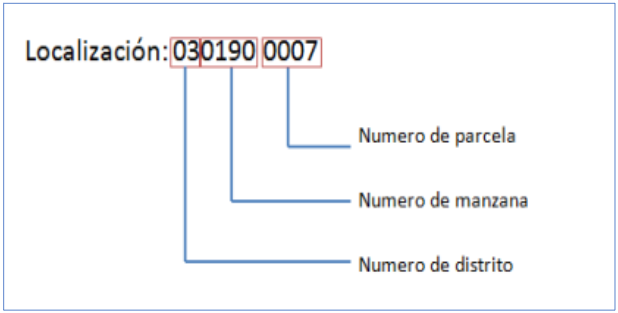
\includegraphics[scale=0.5]{Graphics/localizacion_predio.png}
                  \caption{Descripción y delimitación del número de localización de un predio.} % Título de la figura
                  \label{fig:figura1}
            \end{figure}
\end{itemize}
Por ende el problema de este trabajo puede ser enunciado como la carencia de una
aplicación móvil que permita automatizar el proceso de encuesta a propiedades y
recogida de información mediante formularios, que además cumpla con los
requerimientos funcionales, no funcionales y de entorno planteados anteriormente.
Dando paso a la siguiente pregunta científica:
\textbf{¿Será posible desarrollar una aplicación móvil que cumpla con los requerimientos
      planteados en este epígrafe y así dar solución al problema planteado?}




\section{Objetivos generales y específicos} \label{section:objetivosGeneralesYEspecificos}
Como objetivo general se tendrá desarrollar una aplicación que permita a los
encuestadores auditar los predios mediante el uso de formularios que permitan
recoger información sobre dichos predios, caracterizando los mismos en base a los
cinco módulos: Edificación, Terreno, Construcción, Uso de Patentes/Licencias
Comerciales y Medidores eléctricos; y además agregue funcionalidades como
podrían ser optimizar el camino que debe recorrer el consultor para visitar los
predios que le fueron asignados. De aquí se derivan varios objetivos específicos o
parciales:
\begin{itemize}
      \item Investigar las distintas plataformas para el desarrollo de aplicaciones móviles.
            Ventajas y desventajas.
      \item Analizar las herramientas existentes para el trabajo con mapas en
            concordancia con el entorno de desarrollo seleccionado y que permita
            visualizar cartografía offline.
      \item Diseñar una arquitectura extensible, haciendo uso de los principios del
            desarrollo SOLID\footnote{En programación, SOLID es un acrónimo que representa cinco principios de diseño de software: Responsabilidad Única, Abierto/Cerrado, Sustitución de Liskov, Segregación de Interfaces e Inversión de Dependencias. Estos principios buscan facilitar la creación de código más limpio, mantenible y extensible. } y empleando las buenas prácticas.
      \item Brindar mecanismos de acceso a los sensores del dispositivo móvil para una
            recopilación de datos más completa, dígase GPS2
            , cámara, como los
            principales.
      \item Cumplir con los requerimientos de la aplicación móvil pedida por el
            cliente.
\end{itemize}

\section{Estructura del trabajo}
Este trabajo está compuesto por cuatro capítulos estructurados de la siguiente
manera:
\begin{itemize}
      \item Capítulo I: El primer capítulo presenta una breve introducción al tema, la
            motivación y justificación del mismo, la formulación del problema y los objetivos
            principales, concluyendo este capítulo con la estructura del trabajo.
            2 Sistema que permite posicionar cualquier objeto sobre la Tierra con una precisión de hasta
            centímetros, aunque lo común son unos pocos metros.
            1 Acrónimo que agrupa 5 principios clave para el desarrollo eficiente, replicable, mantenible y
            escalable de software.
      \item Capítulo II: Acá se analizan diferentes sistemas que ofrecen funcionalidades
            similares a la propuesta a desarrollar con el objetivo de explicar sus ventajas y
            desventajas. Se analizan además diferentes plataformas para el desarrollo de
            aplicaciones móviles y algunas tecnologías para el trabajo cartográfico.
      \item Capítulo III: Se verifica de una manera teórico-computacional la propuesta de
            solución. Además se dan algunos detalles de implementación que se consideran
            atractivos de explicar.
      \item Capítulo IV: En este capítulo se muestra el correcto funcionamiento del software
            creado y el cumplimiento de los objetivos del trabajo, con varias pruebas que se le
            hacen a la aplicación y a las distintas herramientas implementadas. Por último
            contamos con las conclusiones y recomendaciones de esta tesis.
\end{itemize}


\chapter{Estado del Arte}\label{chapter:state-of-the-art}

En este capítulo, se hará un bogeo de actualidad, tanto por las diferentes aplicaciones que tienen funcionalidades
que podrían acercarse lo que se necesita, como por las posibles plataformas donde desarrollar el software en cuestión,
seleccionando una de ellas para el desarrollo de la aplicación y las librerías que se emplearán para el trabajo con mapas.

\section{Herramientas similares}






\subsection{geojson.io}
\begin{figure}[h]
    \centering
    
\includegraphics[scale=1.5]{Graphics/geojson.io_logo.png}
    \caption{Logo del servicio web geojson.io.}
    \label{fig:figura3}
\end{figure}
Geojson.io \cite*{geojson.io} es un servicio o aplicación web muy útil. Es totalmente gratis y bien conocido en toda la comunidad
de desarrolladores y personas que usan Sistemas de información geográfica hoy en día.
Esta aplicación web se centra en, como ya su
nombre lo deja saber, hacer más fácil la estructuración, visualización y el solapado de archivos que contienen información geográfica vectorial.
Dicha información vectorial es visualizada de manera intuitiva y minimalista en un mapa con muy buen aspecto visual usando el servicio
de mapas de MapBox \cite{mapbox}. El formato de archivo que por excelencia se utiliza para almacenar información geográfica vectorial es \textit{geojson} \cite*{geojsonOfficialPage}.
geojson.io también permite agregar metadatos a los archivos, lo cuál es una característica muy útil para esta información espacial ya almacenada en los archivos.
Como se podrá observar en la siguiente figura(ver figura \ref{fig:figura4}), en un lateral de la pantalla se tiene el mapa y en el otro dos tipos de vistas, la de archivo de texto plano(formato geojson)
y una vista tabular que es bastante útil a la hora de rellenar información sobre las entidades.
\begin{figure}[h]
    \centering
    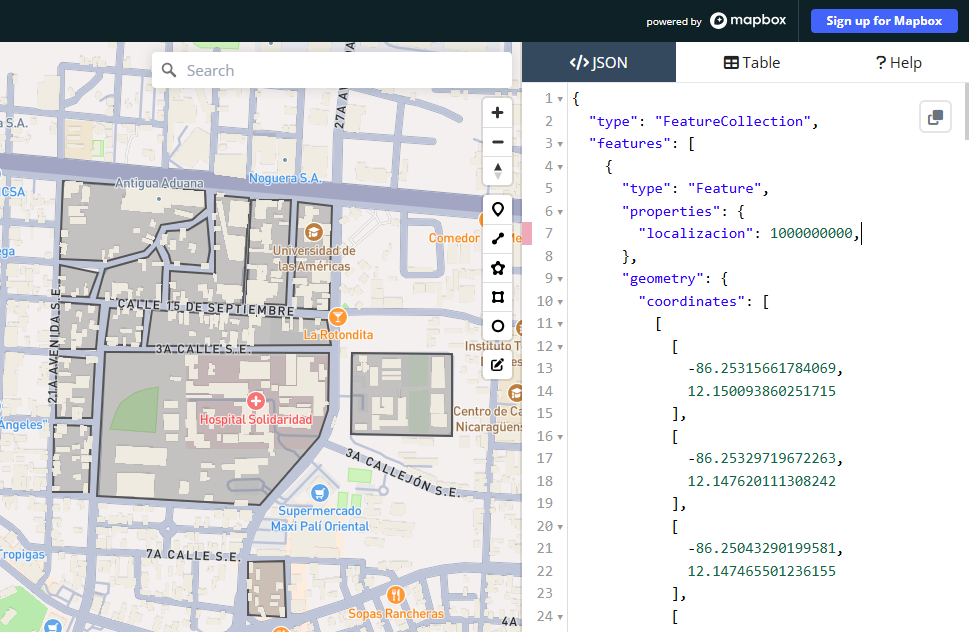
\includegraphics[scale=0.5]{Graphics/geojson.io_description.png}
    \caption{Vista de utilización del servicio geojson.io.}
    \label{fig:figura4}
\end{figure}
Acercándonos al problema de esta tesis, esta página podría resolver varios problemas y puede servir como herramienta para el preprocesado de los datos, como se verá más
adelante en el Capítulo \ref{chapter:proposal}, pero tiene varios aspectos que la alejan de dar solución a lo que necesitamos. Entre los puntos con los que no cumple este servicio
para la solución que se necesita están:
\begin{itemize}
    \item El mapa es cargado con conexión a internet.
    \item No se pueden agregar campos personalizados de tipo fehca o imagen a los metadatos que sirvan luego para almacenar la información que necesitamos de las entidades a encuestar.
    \item No es cómodo acceder a la página desde un dispositivo móvil por el tamaño de la pantalla y, rellenar información ya sea en un archivo de texto plano como lo es geojson o incluso en la vista de tabla puede ser bastante engorroso.
    \item No se puede establecer una relación entre un solo terreno y varias entidades pertenecientes al mismo. Esto es un requerimiento básico del modelo de datos del problema en cuestión.
\end{itemize}






\subsection{Google My Map}
\begin{figure}[h]
    \centering
    
\includegraphics[scale=0.5]{Graphics/google_my_maps_logo.png}
    \caption{Logo del servicio web Google My Maps.}
    \label{fig:figura5}
\end{figure}
Google My Maps \cite{googleMyMaps} es un subdominio del servicio Google Maps, el cuál fue creado como una funcionalidad adicional para permitir a los usuarios
crear sus propios mapas personalizados. Este es un servicio muy parecido a geojson.io, con la diferencia de que aquí es posible agregar campos con imágenes, fechas o de Verdadero/Falso.
También se tiene una vista tabular un poco más intuitiva, aunque aún hay condiciones del problema que no son suplidas con este servicio:
\begin{itemize}
    \item El mapa es cargado con conexión a internet.
    \item No es posible rellenar datos sobre diferentes tuplas relacionadas a un mismo terreno.
    \item Sigue proveyendo un formulario estático, el cuál habría que exportar e importar constantemente para preservar los datos.
\end{itemize}
\begin{figure}[h]
    \centering
    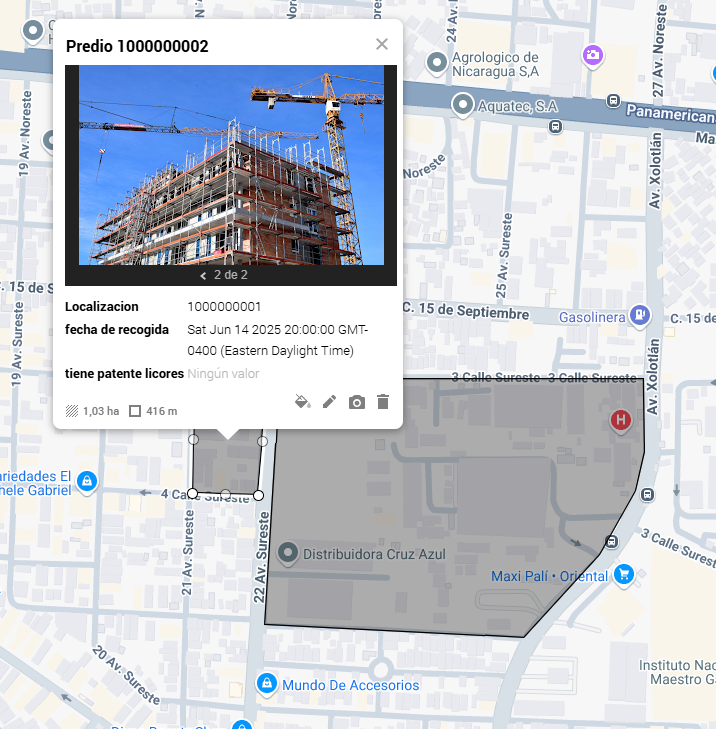
\includegraphics[scale=0.5]{Graphics/google_my_maps_descripcion.png}
    \caption{Vista de utilización del servicio Google My Maps.}
    \label{fig:figura6}
\end{figure}

\pagebreak








\subsection{SW Maps}

\begin{figure}[h]
    \centering
    
\includegraphics[scale=0.5]{Graphics/sw_maps_logo.png}
    \caption{Logo de la aplicación SW Maps.}
    \label{fig:figura7}
\end{figure}
SW Maps es una aplicación móvil de Sistemas de Información Geográfica (SIG) orientada a la recolección de datos espaciales en campo. Desarrollada para plataformas Android, permite capturar, visualizar y editar información geográfica utilizando tanto el GPS interno del dispositivo como receptores GNSS externos, proporcionando así flexibilidad y precisión en el levantamiento de datos.\\\\
Funcionalidades principales:
\begin{itemize}
    \item Creación y edición de entidades espaciales (puntos, líneas y polígonos).
    \item Definición de formularios personalizados para la captura de atributos asociados a cada entidad.
    \item Compatibilidad con diversos formatos de datos geoespaciales: MBTiles, GeoJSON, CSV, entre muchos otros.
    \item Soporte para superposición de capas raster (imágenes georreferenciadas) y capas vectoriales.
    \item Conectividad con servicios de mapas en línea (OpenStreetMap, Google Maps, etc.).
    \item Posibilidad de operar completamente offline, permitiendo el trabajo en áreas sin conectividad.
    \item Exportación de datos recolectados para su posterior análisis en plataformas SIG de escritorio como QGIS \cite*{qgis}.
\end{itemize}

\begin{figure}[h]
    \centering
    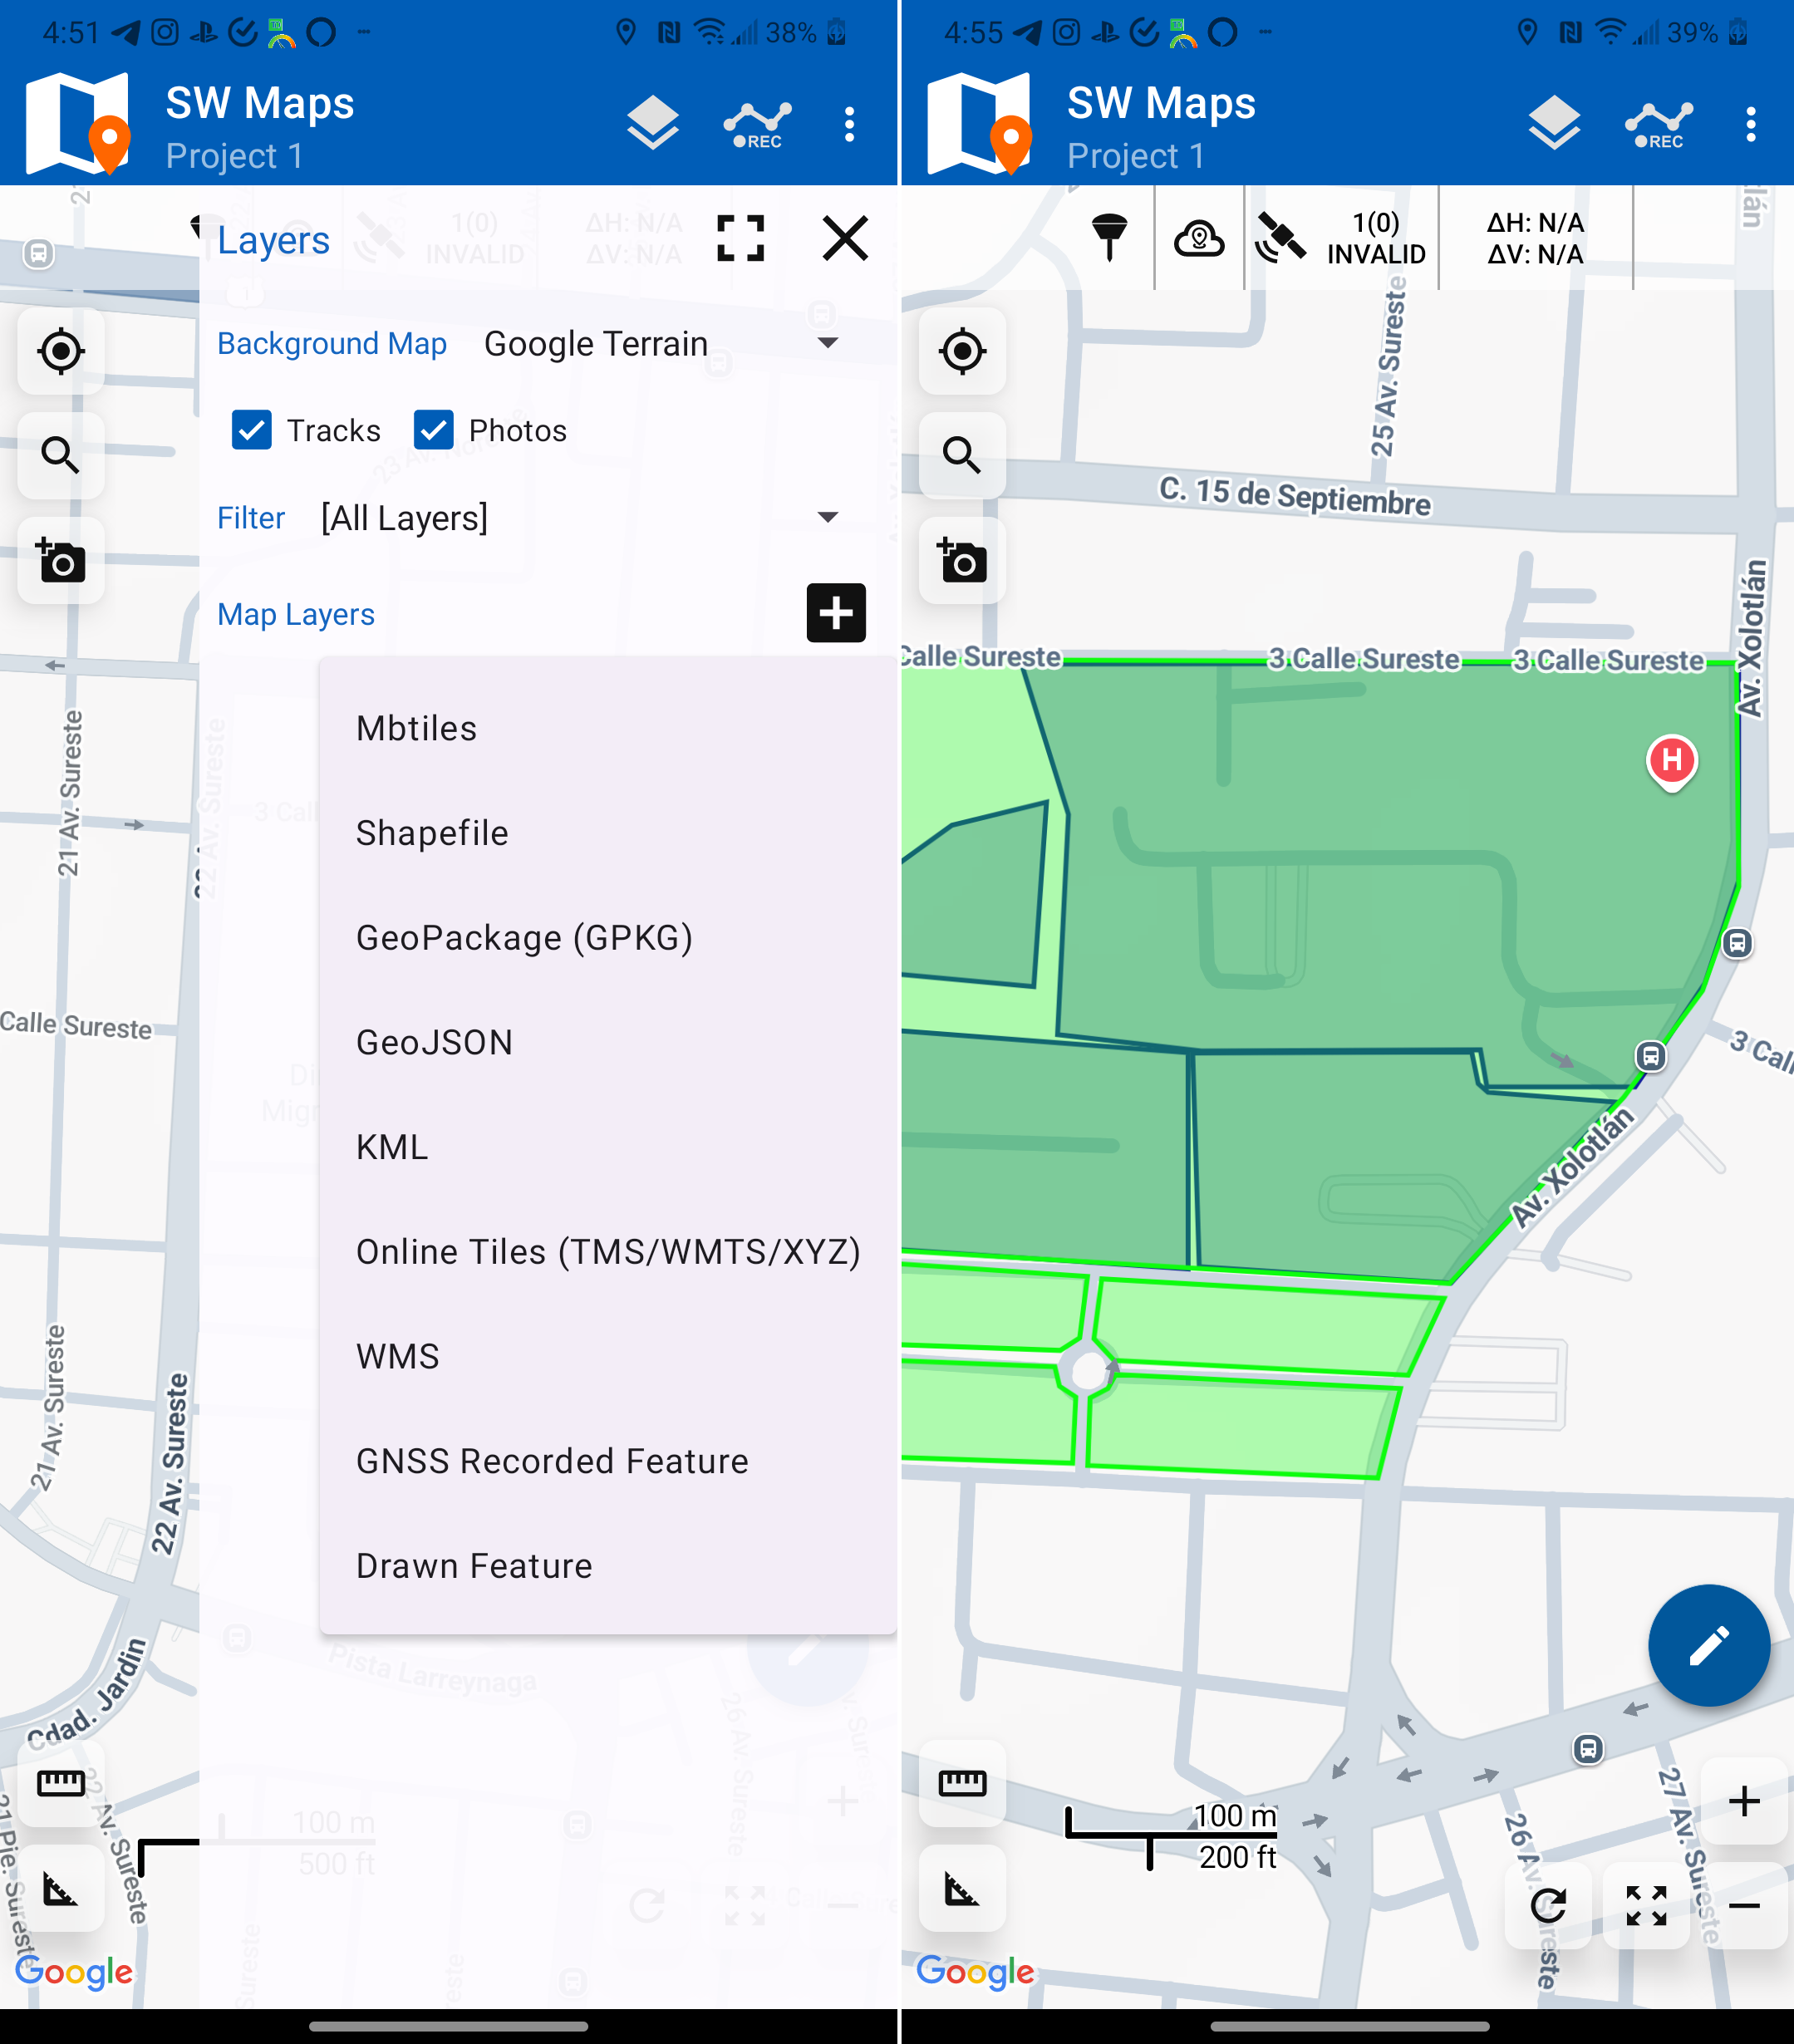
\includegraphics[scale=0.15]{Graphics/sw_maps_importacion.png}
    \caption{Variantes de importación en la aplicación SW Maps.}
    \label{fig:figura8}
\end{figure}

SW Maps es la solución más cercana y conveniente que se encontró en cuanto a solución de los requerimientos del problema. Esta aplicación para Android
tiene la posibilidad de importar y exportar datos geográficos, alimentar estos datos georreferenciadas con metadatos que se rellenan en formularios con una
validación bastante descente, con campos de Verdaero/Falso, imágenes, numéricos e incluso selección simple y selección múltiple.

\begin{figure}[h]
    \centering
    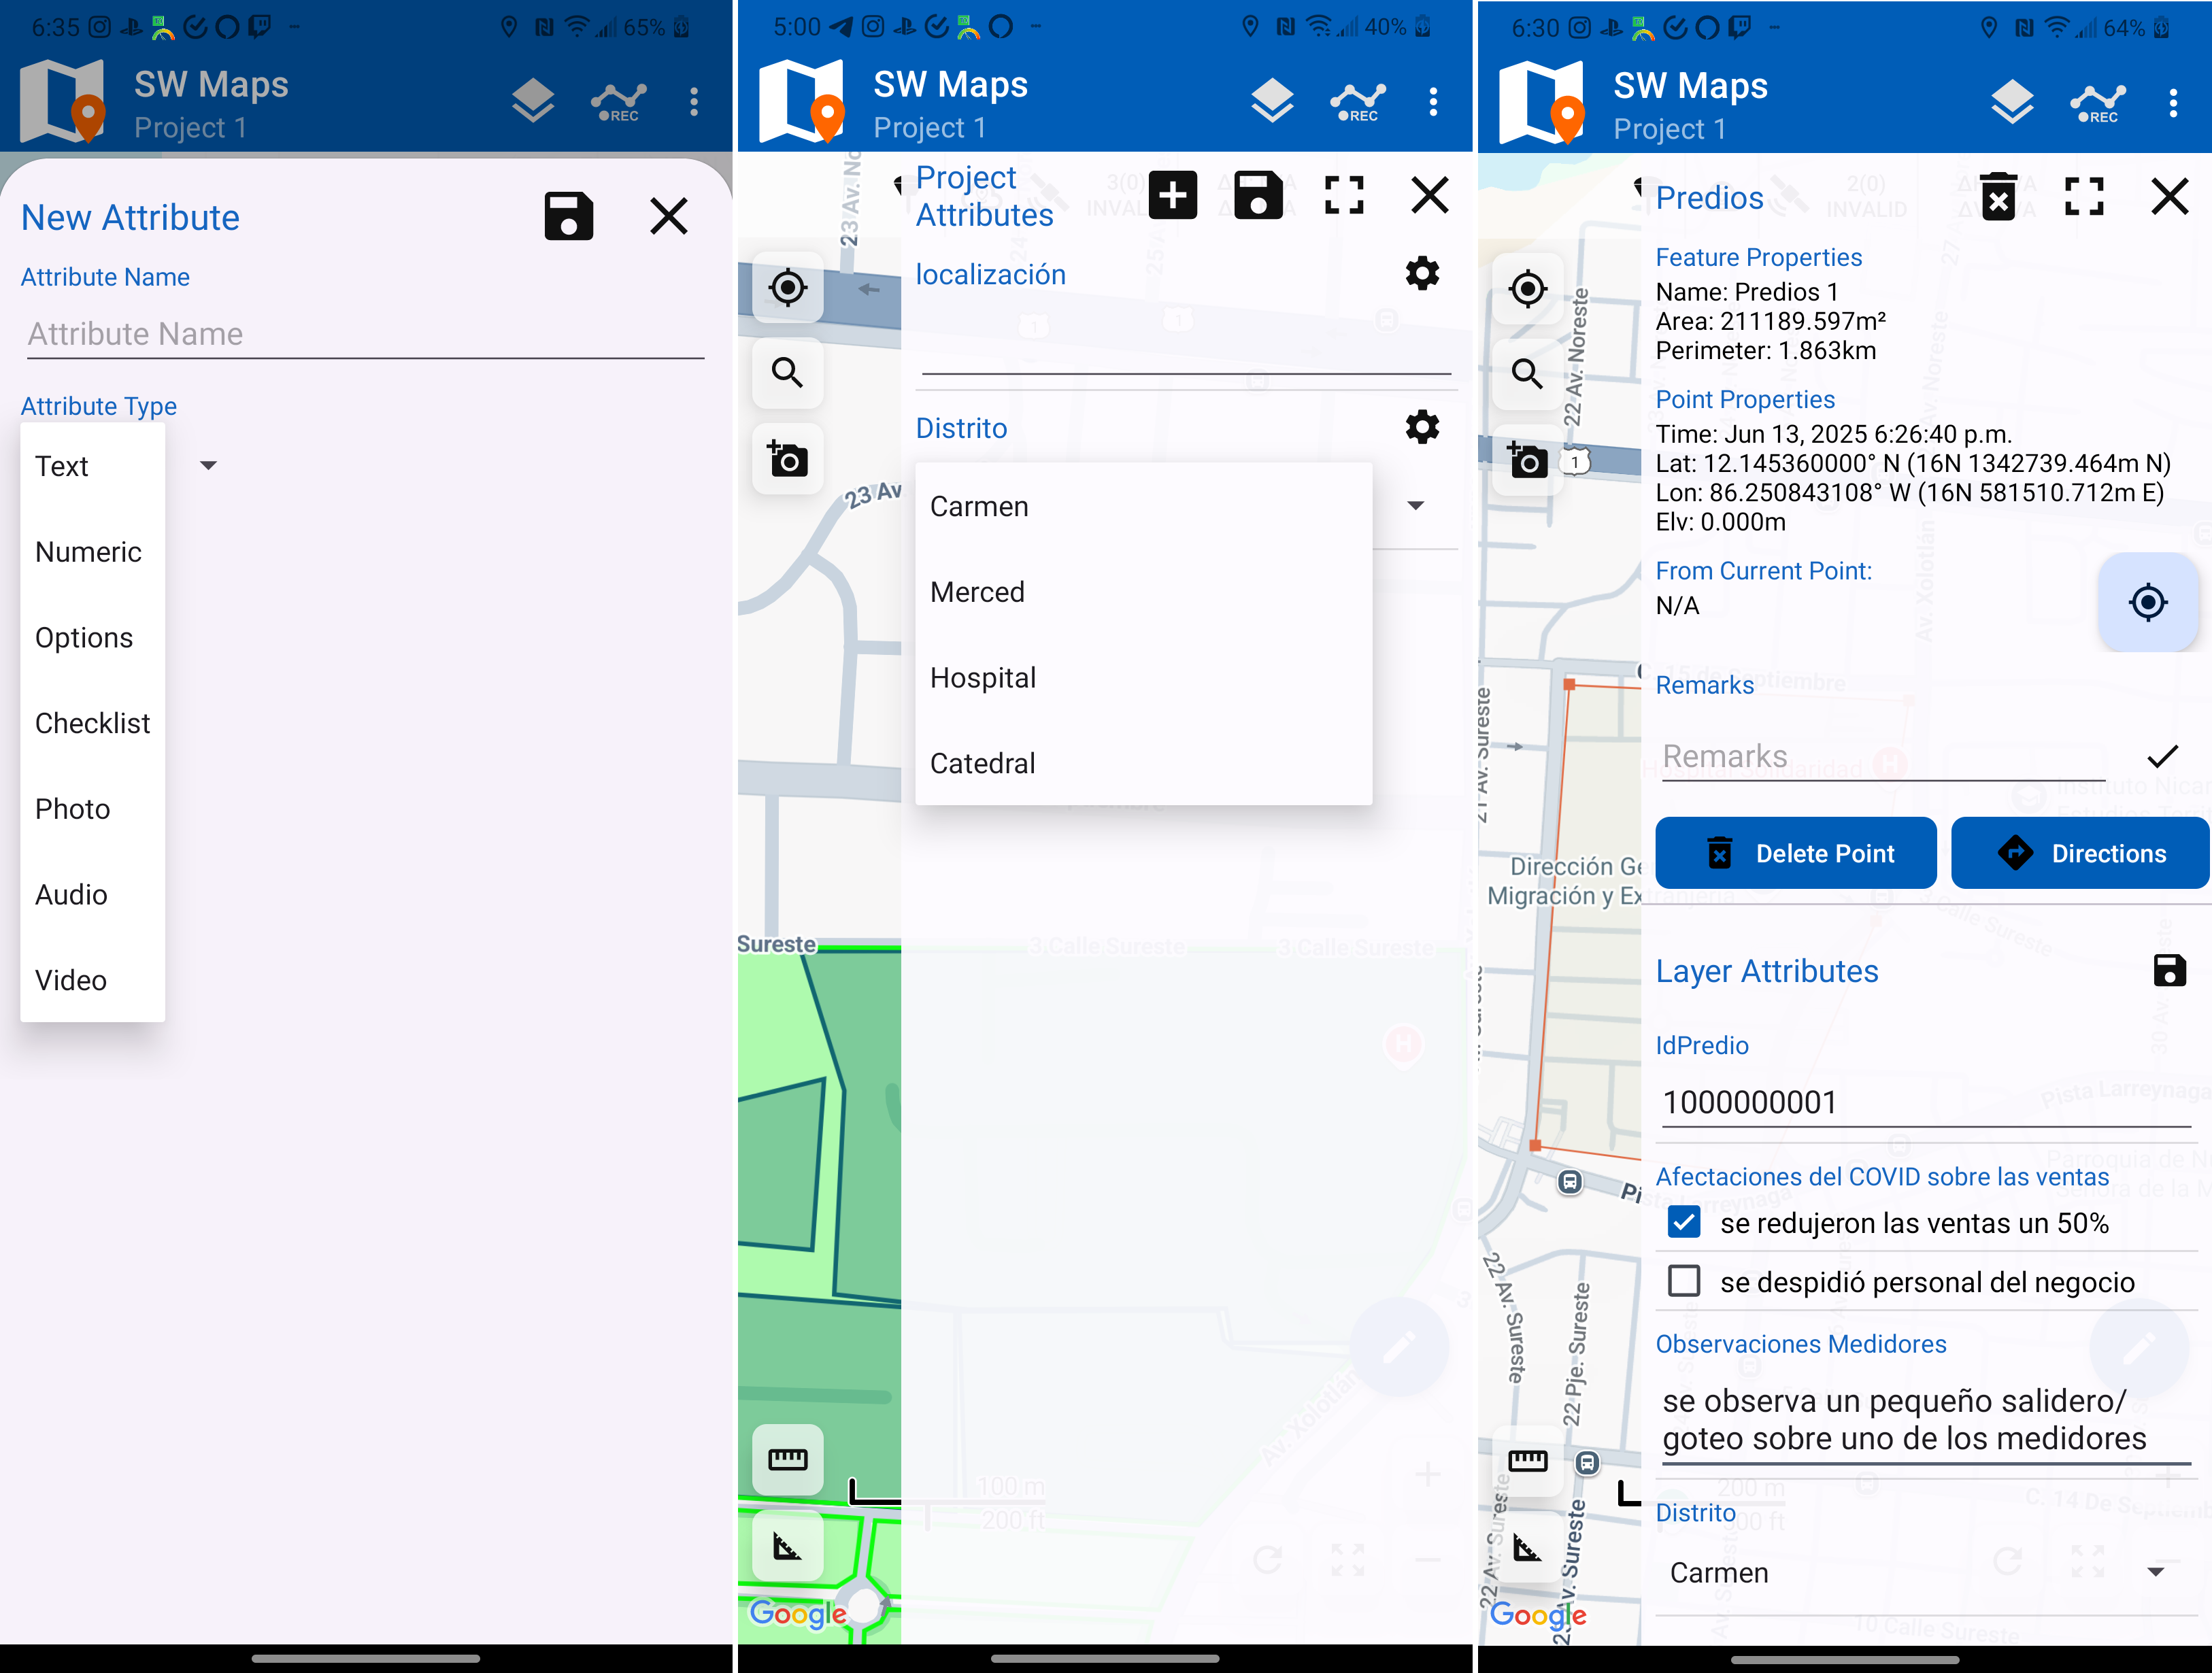
\includegraphics[scale=0.15]{Graphics/sw_maps_campos.png}
    \caption{Variantes de campos de formularios en la aplicación SW Maps.}
    \label{fig:figura9}
\end{figure}

Pero luego de un análisis muy breve se puede observar que esta aplicación tampoco se encuentra ni cerca de ser una posible variante de solución:
\begin{itemize}
    \item Sigue sin ser posible establecer una relación entre un terreno y varias propiedades pertenecientes a la misma área, como lo son las propiedades o locales de diferentes pisos de un mismo edificio. Como ya se dijo, esto es un requisito básico de la naturaleza y los datos del problema.
    \item No se puede hacer ningún tipo de validación extra, que tenga en cuenta por ejemplo, que el número de localización de un predio debe tener específicamente 10 cifras, o que al activar el campo "tiene más patentes" se desbloquea el campo "número de patente 2"
    \item El campo fecha tendría que ser simulado con un campo numérico o de texto, lo cuál no es muy amigable con el usuario y da lugar a que se puedan cometer errores al rellenar este tipo de campos.
    \item No sería posible añadir características intrínsecas de la lógica de negocio del problema, como lo es por ejemplo, que al rellenar los datos de un terreno, este pueda marcarse con otro color para ayudar a los encuestadores a tener una guía de qué terrenos han visitado hasta el momento; lo cuál es una de las razones principales por las que la aplicación solución debe incluir un mapa.
\end{itemize}







\subsection{Conclusiones sobre las diferentes herramientas expuestas}
En esta sección se analizaron aplicaciones con objetivos similares a la aplicación que
se desea desarrollar explicada en el capítulo anterior. Este análisis se realizó con el objetivo
de hacer certera la necesidad de desarrollar una aplicación para Android desde cero. Podemos, dado el análisis anterior, llegar a los siguientes hechos:
\begin{enumerate}
    \item Las herramientas que se exploraron en general no están acorde con las necesidades planteadas por el problema.
          \begin{enumerate}
              \item Muchos de los visores de mapas con que cuentan las aplicaciones analizadas necesitan de
                    internet para mostrar la cartografía. Esto incumple con uno de los requerimientos del cliente.
              \item Muchas de las aplicaciones SIG genéricas están diseñadas con el propósito de rellenar información sobre porciones de terreno, pero en ocasiones se necesita tener no solo información del terreno en general, sino también de los edificios de ese terreno y las propiedades individuales de esos edificios. En este caso es necesario hacer uso de bases de datos relacionales para el correcto almacenamiento de las entidades respresentadas en los datos del problema.
              \item Para una experiencia personalizada de validación de formularios, es preferible y en la mayoría de casos necesario implementar una aplicación desde cero.
          \end{enumerate}
\end{enumerate}
Luego de analizar las aplicaciones anteriores se concluye como necesario el diseño e
implementación de una aplicación que sí cumpla con los requerimientos expuestos en este documento.

\section{Tecnologías de desarrollo de aplicaciones para Android}
\subsection{.NET MAUI}
\begin{figure}[h]
    \centering
    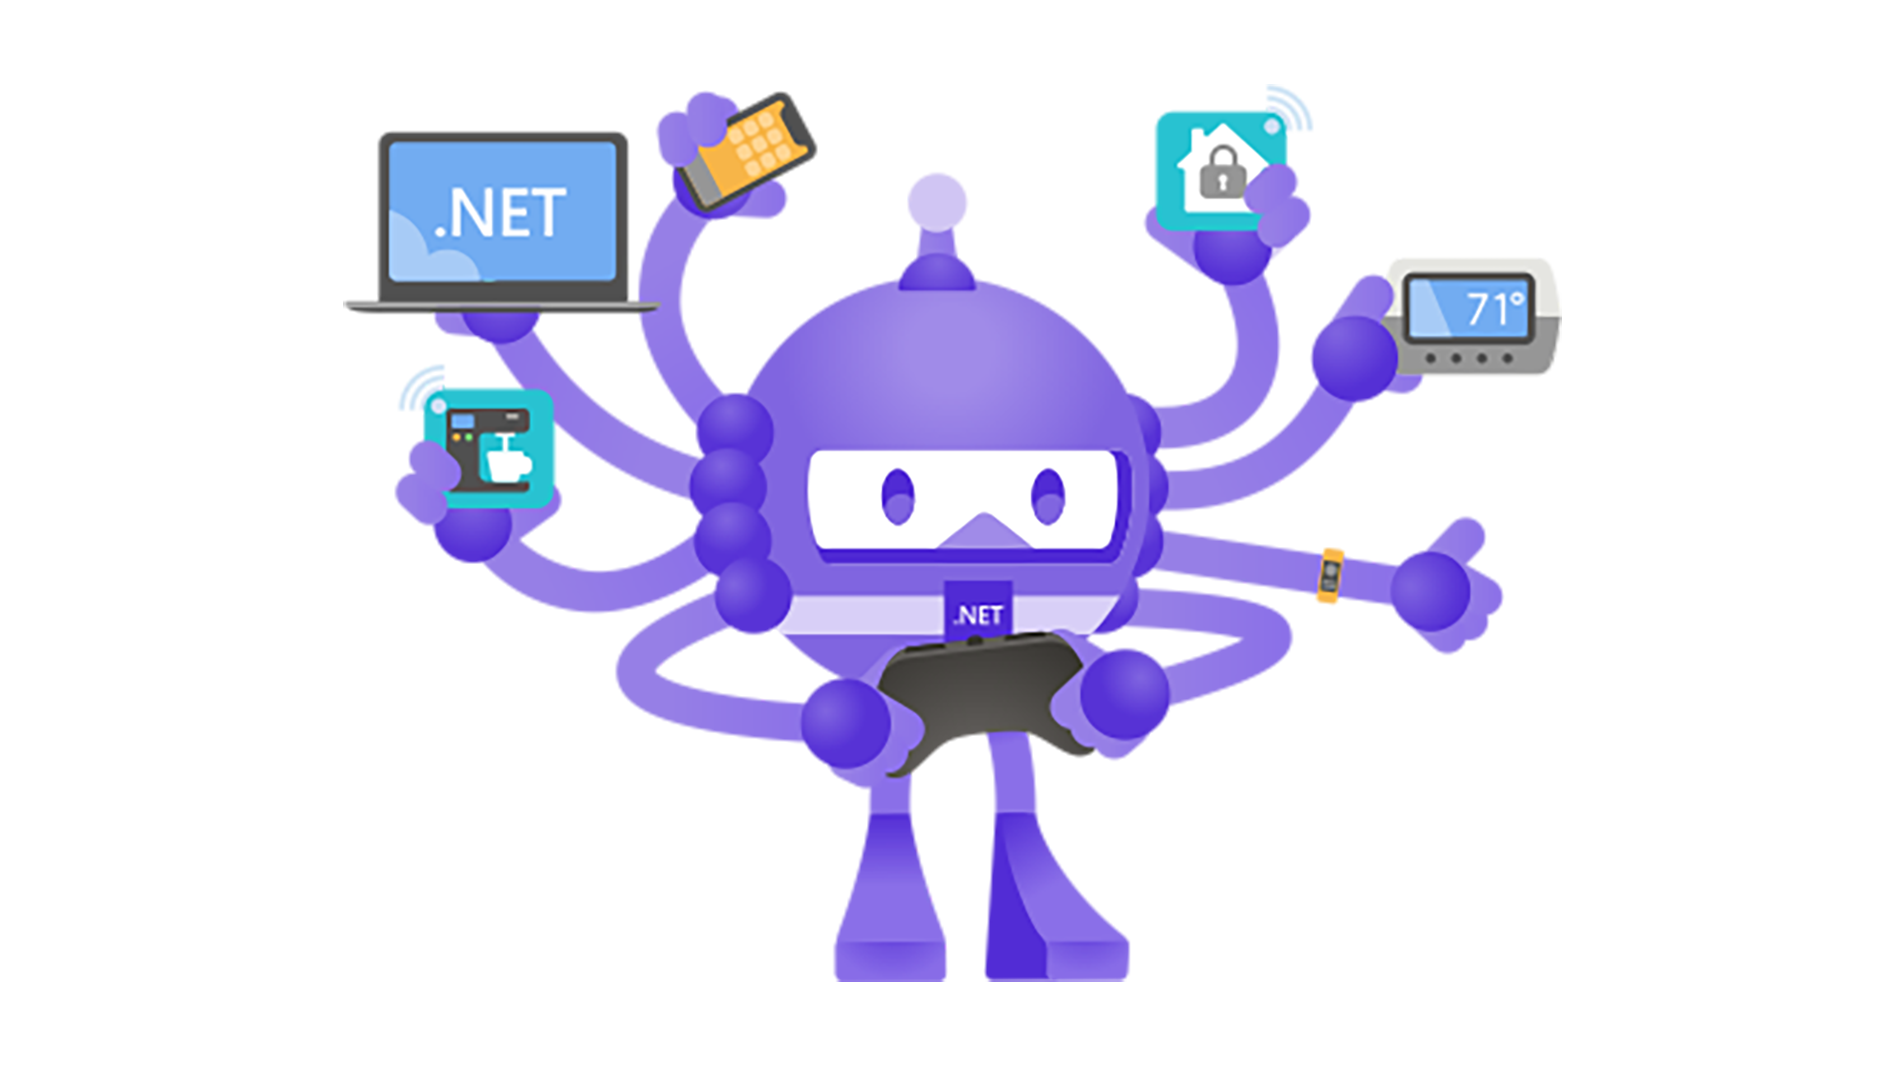
\includegraphics[scale=0.15]{Graphics/MAUI.png}
    \caption{Logo de MAUI.}
    \label{fig:figura10}
\end{figure}
.NET MAUI (Multi-platform App UI) es el framework de desarrollo multiplataforma más reciente de Microsoft, lanzado oficialmente en 2022 como evolución directa de Xamarin.Forms. Forma parte integral del ecosistema .NET 6+.
y permite desarrollar aplicaciones nativas con un único código base para Android, iOS, Windows y macOS
Su arquitectura permite compartir la lógica de negocio, la interfaz de usuario y los recursos entre todas las plataformas, utilizando C\# y XAML como lenguages de programación para el desarrollo.
MAUI unifica los proyectos en una sola estructura de proyecto multiobjetivo, haciendo fácil la administración del código. Compila a código nativo de cada plataforma, accediendo directamente a las APIs nativas sin necesidad de la generación de código intermedio.
Este framework aprovecha la gran comunidad consolidada de desarrolladores .NET y C\# y la comunidad de Xamarin que ha migrado progresivamente hacia acá.
Hay que destacar que Visual Studio ofrece un entorno muy integrado con MAUI a este momento por lo que es una oferta tentadora dada la gran base en el lenguaje C\# proveniente de la carrera.
Destacar el soporte nativo para patrones modernos como MVVM, lo cuál sería una gran tentativa también ya que es la arquitectura escogida para el desarrollo de la aplicación.\\\\
Desventajas:
\begin{itemize}
    \item Aunque hereda parte de la comunidad Xamarin, su base de usuarios aún es más pequeña que Flutter o React Native en el ámbito multiplataforma.
    \item Limitada penetración fuera del ecosistema Microsoft y empresas tradicionales de desarrollo empresarial.
    \item Aunque ha mejorado, la productividad para diseñar UI complejas sigue siendo inferior en comparación con frameworks declarativos como Flutter.
    \item El diseño con XAML puede resultar más verboso y menos intuitivo para nuevos desarrolladores.
    \item Ecosistema de plugins más reducido respecto a Flutter o React Native (aunque en crecimiento).
\end{itemize}

\subsection{React Native}
\begin{figure}[h]
    \centering
    
\includegraphics[scale=0.15]{Graphics/react_native_logo.png}
    \caption{Logo de React Native.}
    \label{fig:figura11}
\end{figure}
React Native es un framework de desarrollo de aplicaciones móviles multiplataforma creado originalmente por Facebook (hoy Meta). Permite desarrollar aplicaciones para Android e iOS utilizando JavaScript o TypeScript, empleando el paradigma declarativo de React para construir interfaces de usuario.
El núcleo de React Native traduce los componentes escritos en JavaScript a componentes nativos equivalentes mediante un sistema de puente (bridge), que permite interactuar con las APIs nativas de cada plataforma. A partir de 2022-2023, React Native está evolucionando hacia un modelo de arquitectura denominado Fabric, que reduce la latencia del bridge y mejora el rendimiento en la interacción entre el código JS y el sistema nativo.
React Native permite un alto grado de reutilización de código, especialmente en la lógica de presentación y en las interfaces de usuario, manteniendo acceso a módulos nativos cuando es necesario para funcionalidades específicas de cada plataforma.
Una de sus ventajas es que tiene una de las comunidades de desarrollo móvil más grandes y activas, una super amplia disponibilidad de documentación, tutoriales, librerías y plugins y además el hecho de ser un ecosistema abierto, respaldado por Meta y miles de contribuyentes en internet.
Posee una gran cantidad de paquetes listos para uso en proyectos reales (navegación, mapas, bases de datos, formularios, etc.) así como una programación clara y minimalista en forma declarativa con React. Otra de las ventajas a considerar de este framework es que dado el largo tiempo en el mercado y el gran uso en el mundo real, se sostiene una compatibilidad constante con nuevas versiones de Android e iOS.\\\\
Desventajas:
\begin{itemize}
    \item A pesar de tener una comunidad de desarrolladores muy numerosa, la calidad de algunas librerías de terceros es desigual; muchas no están siempre bien mantenidas.
    \item Dificultad a veces para encontrar soluciones "oficiales" cuando no existe un paquete bien soportado.
    \item Gestión de dependencias puede complicarse cuando hay múltiples paquetes con actualizaciones incompatibles.
    \item Algunas funciones específicas de hardware o SDKs nativos (por ejemplo, ciertos SDKs de cámaras, sensores avanzados o SDKs comerciales cerrados) pueden requerir escribir módulos nativos (en Java/Kotlin para Android o Swift/Obj-C para iOS).
    \item Cambios frecuentes en versiones mayores (por ejemplo: de la arquitectura clásica al nuevo Fabric) que obligan a adaptarse.
    \item Dependencia del ecosistema Node.js puede generar conflictos de versiones de paquetes.
\end{itemize}


\subsection{Flutter}
\begin{figure}[h]
    \centering
    
\includegraphics[scale=0.15]{Graphics/flutter_logo.png}
    \caption{Logo de Flutter.}
    \label{fig:figura12}
\end{figure}
Flutter es un framework de desarrollo de aplicaciones multiplataforma creado por Google. Permite desarrollar aplicaciones nativas para Android, iOS, Web, Windows, macOS y Linux utilizando un único código base escrito en el lenguaje Dart.
A diferencia de otros frameworks que utilizan un puente (bridge) como se vio anteriormente con React Native, entre el código y las APIs nativas, Flutter renderiza directamente los componentes de interfaz de usuario mediante sus propios motores gráficos (Skia/Impeller), controlando cada píxel de la pantalla. Esto le permite ofrecer una experiencia visual coherente, personalizable y con alto rendimiento en todas las plataformas.
Además de la interfaz de usuario, Flutter permite integrar lógica de negocio, acceso a dispositivos, bases de datos, servicios en la nube y SDKs nativos, mediante canales de plataforma (platform channels) o plugins desarrollados en la propia comunidad.
Hace unos años, desde su primera versión, el desarrollo en esta plataforma ha ido creciendo exponencialmente. Una de las ventajas más fuertes que puede tener Flutter es el respaldado por Google, con fuerte inversión continua en desarrollo y documentación.
Muy buena documentación y Tutoriales en sus plataformas oficiales.
Posee una interfaz de usuario declarativa y reactiva, lo cuál junto con la facilidad de depuración del código lo hacen una gran opción. Posee una gran cantidad de widgets preconstruidos para interfaz de usuario y de paquetes oficiales y de la comunidad disponibles vía pub.dev.\\\\
Desventajas:
\begin{itemize}
    \item Aunque es una de las comunidades que más crece, aún hay menor cantidad de desarrolladores senior comparado con tecnologías como React Native o el ecosistema Android nativo.
    \item Al ser relativamente reciente (2018), algunos escenarios muy específicos aún dependen de la comunidad para ser bien soportados.
    \item La curva inicial de aprendizaje de Dart puede representar un pequeño obstáculo para programadores que provienen de JavaScript o Java.
    \item Para ciertas personalizaciones nativas avanzadas, es necesario desarrollar código nativo en Kotlin/Swift y manejar los Platform Channels.
    \item La dependencia en la calidad de los plugins de terceros puede generar riesgos si algunos quedan desactualizados.
    \item Proyectos muy grandes pueden volverse difíciles de mantener si no se adopta desde el inicio un patrón arquitectónico sólido.
    \item Algunos conceptos (por ejemplo: manejo de estado, inyección de dependencias, modularización) requieren decisiones de arquitectura bien pensadas desde temprano.
\end{itemize}

\subsection{Conclusiones sobre las plataformas de desarrollo expuestas}
Teniendo en cuenta las ventajas y deficiencias en cada uno de los frameworks anteriormente expuestos, hay que decir que las tres plataformas tienen sus ventajas pero Flutter será la escogida
para la implementación de la aplicación dadas todas las ventajas antes expuestas, pero además las necesidades específicas de la implementación que se realizará, dado que se necesita una alta reactividad
en los campos de formularios, ya que se pretende tomar una vertiente moderna y reactiva de la idea de un formulario. Con el potente motor gráfico de Flutter se puede obtener un alto rendimiento en la interfaz.
Este será necesario dada la carga que representa la renderización de mapas, encima con datos geoespaciales personalizados encima, y la función de formularios en la misma zona de ejecución. Flutter es un
framework no tan inexplorado como MAUI y al mismo tiempo viene a resolver deficiencias de React Native, ya que está inspirado en este framework; por lo tanto es una opción razonable e inteligente esta elección.
\section{Librerías para uso de mapas}
\subsection{Librería flutter\_map}
Una implementación en Dart de Leaflet (biblioteca de JavaScript de código abierto
para mapas interactivos aptos para dispositivos móviles) para proporcionar un widget de
mapas para las aplicaciones de Flutter.
El principal atractivo de flutter\_map \cite{flutterMap} en este análisis es la fortaleza y compatibilidad que tiene esta librería con el motor de renderizado
de Flutter, y al unísono, la capacidad de integración con otras librerías que implementan proveedores de teselas, en el caso de la solución a implementar, provenientes de archivos locales
que contengan mapas en el formato que se especificará a continuación.
\subsection{Librería flutter\_map\_mbtiles}
Esta librería proporciona la implementacion de un proovedor de teselas que se configura y carga a partir de archivos locales
en el dispositivo en formato \textbf{.mbtiles}. No solo el proveedor de teselas rasterizadas, sino también capas de polígonos vectoriales y marcadores que son útiles
para la representación de delimitaciones en el mapa, estos a partir polígonos extraídos de archivos en diversos formatos, entre ellos uno de los más populares es \textbf{geojson}.


\subsection{Conclusiones sobre las librerías de mapas}
Se determinó utilizar una combinación de ambas librerías para mostrar tanto el mapa en cuestión como capa base del lienzo, así como también las capas de delimitaciones como
capas extra montadas sobre este mapa base, haciendo uso de la personalización que nos ofrecen estas librerías para hacer marcadores y polígonos informativos que enmarquen
los diferentes predios, manzanas y edificios que se requiran visitar.


\section{Conclusiones del capítulo}
Partiendo de todo lo expuesto en este capítulo de estado del arte resulta importante
resaltar, teniendo en cuenta el estudio de aplicaciones con funcionalidades semejantes
a la deseada, la necesidad de diseñar, desde cero, una aplicación que presente las funcionalidades que se quieren. También consolida la decisión, a partir de los argumentos
expuestos, de tomar como plataforma de desarrollo a Flutter y como gestor de mapas al
paquete flutter\_map cumpliendo con los requerimientos planteados en este documento.

\chapter{Análisis Teórico-Computacional de la propuesta de solución. Detalles de implementación}\label{chapter:proposal}
En el capítulo anterior se realizó un análisis del estado del arte, concluyendo con la
necesidad de implementar desde cero una aplicación de Android usando Flutter para su desarrollo, que cumpla con los requerimientos planteados.
Este capítulo estará enfocado en el marco teórico-computacional de la propuesta de
solución para este proyecto. Se abordarán temas que incluyen los detalles de la arquitectura seleccionada, la modelación de los datos del problema
y el análisis de los requerimientos funcionales de la aplicación. Se abordarán también las principales tecnologías utilizadas, así como, algunos detalles de implementación.
\section{Diagrama de casos de uso}
En esta sección se expondrán las acciones que puede realizar un usuario dentro de la aplicación, explicado a través de un diagrama de casos de uso
\footnote{Diagrama de casos de uso: Forma de diagrama de comportamiento UML(Unified Modeling Language o en español Lenguaje de Modelado Unificado) mejorado. Sirve para
    especificar la comunicación y el comportamiento de un sistema mediante su interacción con los usuarios
    y/u otros sistemas. Un diagrama que muestra la relación entre los actores y los Casos de Uso en un
    sistema.}
, teniendo en cuenta que solo existe un rol de usuario, Encuestador,
y tres grupos de acciones que se encapsulan en el diagrama por comodidad para el lector, Acciones de importación/exportación, Acciones en la pestaña "Mapa" y Acciones en
la pestaña "Registro".
\pagebreak
\begin{figure}[h]
    \centering
    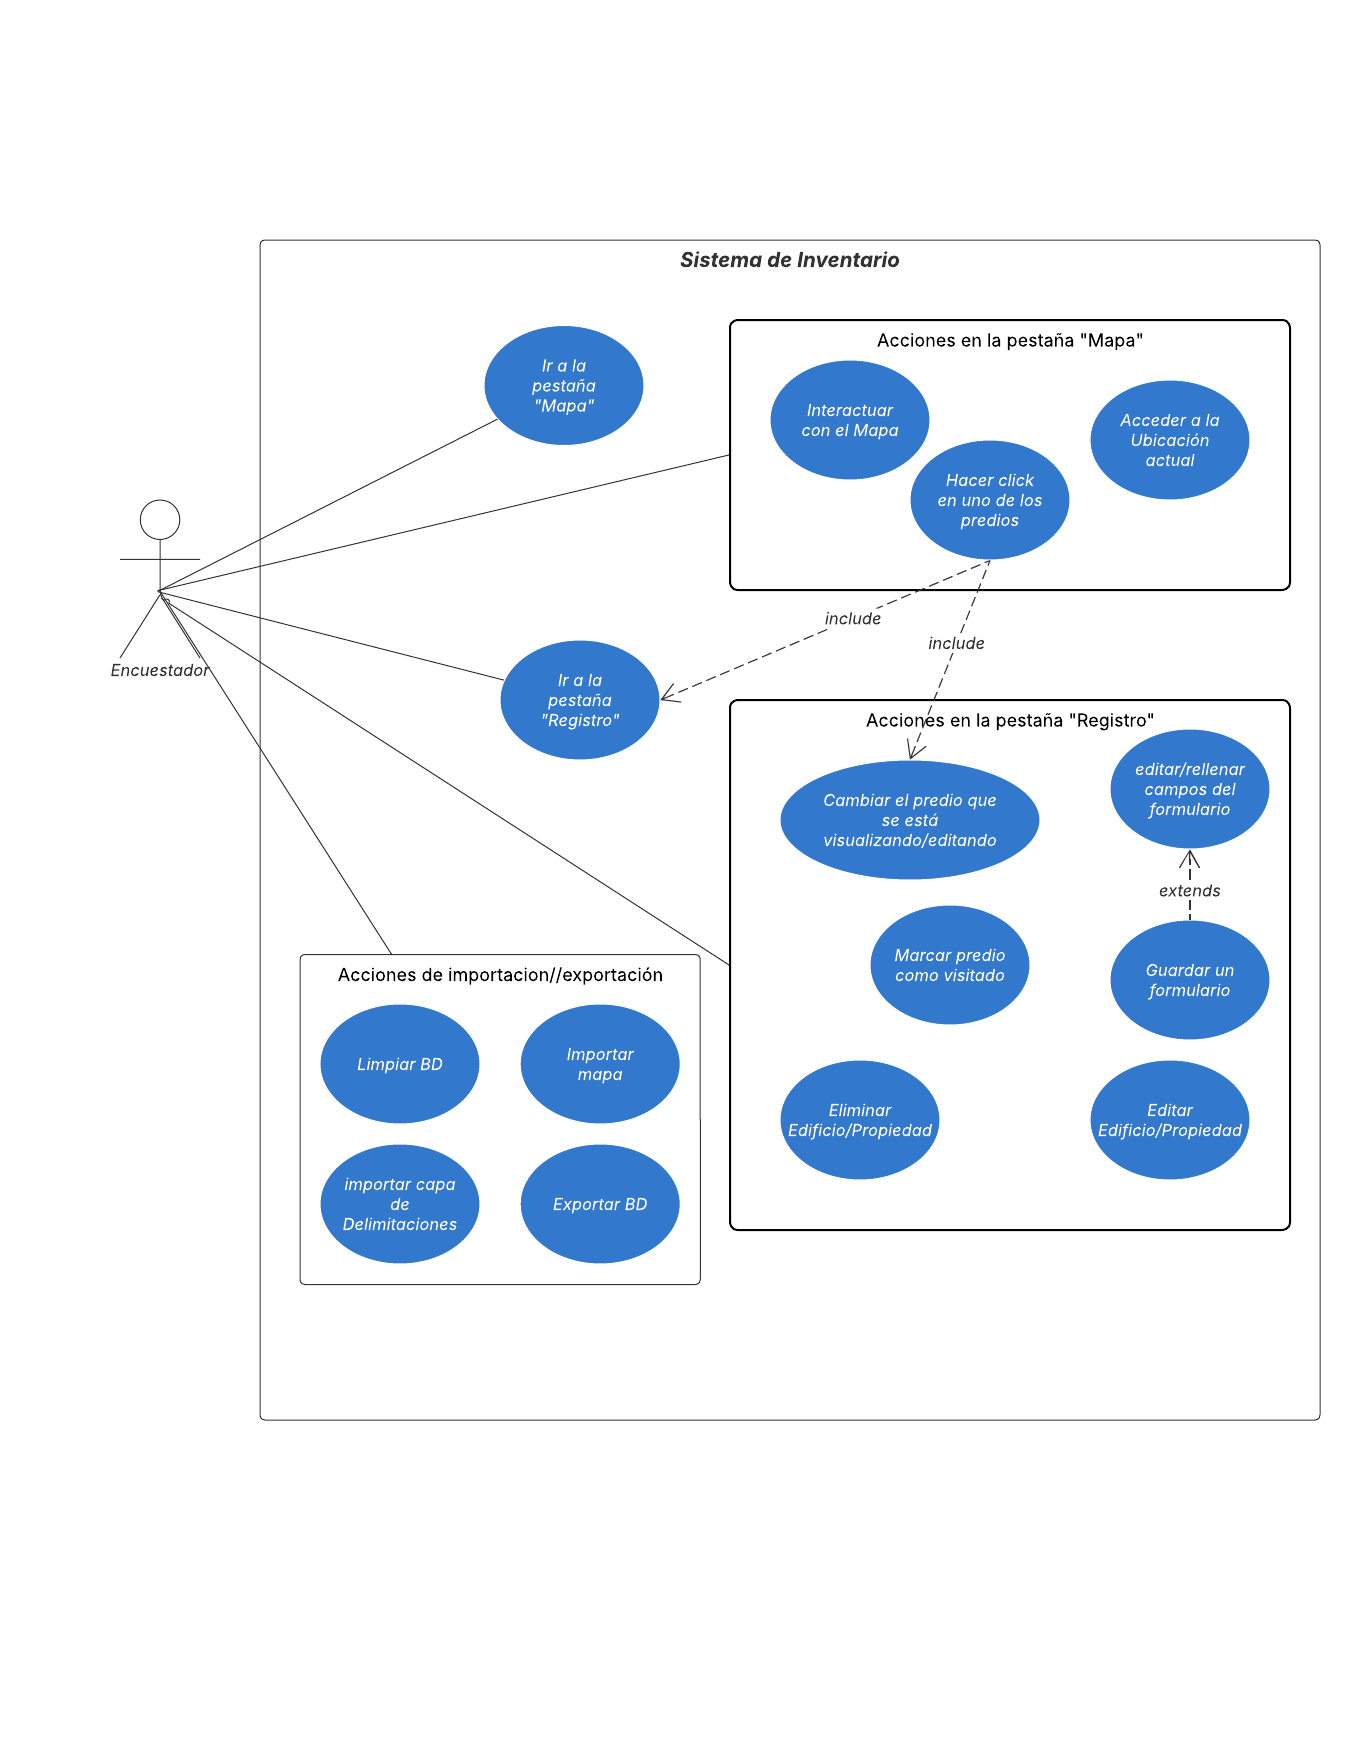
\includegraphics[scale=0.5]{Graphics/Capitulo 3/Diagrama_casos_de_uso.png}
    \caption{Diagrama de casos de uso de la aplicación Inventario.} % Título de la figura
    \label{fig:figura13}
\end{figure}
En la figura anterior(Ver figura \ref{fig:figura13}) se puden observar las diversas acciones que puede realizar un encuestador dentro de
la aplicación. Las mismas se explican a continuación:
\begin{itemize}
    \item \textbf{Ir a la pestaña "Mapa"}: Al presionar en la pestaña nombrada de esta manera se abrirá la vista de Mapa. Por defecto esta es la vista que se muestra.
    \item \textbf{Ir a la pestaña "Registro"}: Al presionar en la pestaña nombrada de esta manera se abrirá la vista de Registro o Formulario. Aquí se podrá introducir información relacionada con los predios, edificios y propiedades que se deseen.
    \item \textbf{Acciones de importación/exportación}
          Aqui se debe recalcar que estas funcionalidades diseñadas puramente por comodidad para los encuestadores, ya que se se colocan el mapa y las
          delimitaciones que se quieren mostrar, en las carpetas correspondientes no será necesario usar más nada, se mostrarán automáticamente en la aplicación.
          \begin{itemize}
              \item \textbf{Importar Mapa}: Esta opción abrirá una nueva ventana de selección de archivos, donde el usuario deberá seleccionar
                    un archivo con extensión ".mbtiles" para importarlo en la aplicación. Esto realizará una copia del archivo seleccionado hacia
                    la carpeta de mapas de la aplicación en el almacenamiento del dispositivo('CADIC/Maps'). Para que la importación surta efecto,
                    se deberá cambiar rápidamente de pestaña o cerrar y abrir la aplicación.
              \item \label{item:importaciongeojson}\textbf{Importar capa de Delimitaciones}: También abrirá una ventana de selección de archivos, pero esta vez esperando que
                    el usuario localice un archivo con extensión ".geojson". Dentro del archivo deben encontrarse definiciones de polígonos, y
                    dentro de cada polígono, en el apartado de "properties" podrá incluirse la etiqueta individual que se deseará mostrar para
                    cada polígono, esta se mostrará en el centro de cada polígono al renderizarse en el mapa. En el caso de una capa de polígonos
                    que representen predios, el archivo que contiene las delimitaciones deberá cumplir 2 resticciones para obtener
                    una correcta integración y funcionamiento con la aplicación. Una de estas restricciones es que el nombre termine de la siguiente manera:
                    \begin{mdframed}
                        (...)\_predios.geojson
                    \end{mdframed}
                    Por ejemplo: "managua\_predios.geojson". La otra restricción es que cada definición de polígono interna en el archivo,
                    tenga una propiedad "localizacion" (sin tilde), con valor igual al número de localización correspondiente al predio que define.
                    De esta manera se importarán correctamente las delimitaciones, considerando cada archivo como una capa, y pintando de un color
                    diferente cada una de estas capas.

              \item \textbf{Exportar BD}: Esto exportará la BD hacia el directorio 'CADIC/Exportado'.
              \item \textbf{Limpiar BD}: Limpia la Base de Datos, solo dejando el nombre del encuestador registrado al iniciar la aplicación por primera vez.
          \end{itemize}
    \item \textbf{Acciones en la pestaña "Mapa"}
          \begin{itemize}
              \item \textbf{Interactuar con el mapa}: En la pestaña "Mapa", la funcionalidad primaria es la interacción con el mapa, lo que abarca desde
                    el acercamiento/alejamiento de la vista del mapa, como el desplazamiento de la vista horizontal y verticalmente. Esto se realiza con
                    los gestos clásicos de navegación por el mapa sobre la pantalla táctil del dispositivo.
              \item \textbf{Hacer click en uno de los predios}: Al cargar las delimitaciones de los predios, edificios y manzanas sobre el mapa,
                    los predios no solo se deberían mostrar como polígonos con borde de color rojo, sino que también deberán tener un marcador visualizado
                    como punto de color negro en su centroide. Al hacer click sobre uno de estos puntos en el mapa, automáticamente se accederá a la información
                    registrada del predio asociado al marcador, abriéndose la vista de la pestaña "Registro" con los datos del predio si había sido registrado previamente.
                    \footnote{El centroide, también conocido como baricentro, es el centro geométrico de una figura o cuerpo. Representa el punto donde se concentraría toda
                        la masa si el objeto tuviera una distribución uniforme de masa. En otras palabras, es el punto de equilibrio de la figura. }

              \item \textbf{Acceder a la ubicación actual}: Si se presiona sobre el botón con un ícono de objetivo, la vista del mapa se centrará en
                    la localización actual del usuario.
          \end{itemize}
    \item \textbf{Acciones en la pestaña "Registro"}
          \begin{itemize}
              \item \textbf{Cambiar el predio que se está visualizando/editando}: Por defecto en la vista del Formulario, el número de Localización no se puede variar,
                    pero al lado de este campo inhabilitado, se encontrará una casilla para marcar, la cuál si está en efecto marcada, permitirá cambiar el número de
                    localización, lo que concede acceder manualmente a la información de un predio con solo introducir su identificador de localización.
              \item \textbf{Editar/rellenar campos del formularios}: Sin profundizar aún mucho en el tema, cabe mencionar que los formularios son reactivos, y por lo tanto,
                    varias acciones que se realicen en la aplicación, tendrán repercución en lo que se muestra y lo que no del formulario.
              \item \textbf{Guardar un formulario}: Un formulario no se registrará en la Base de Datos si no se presiona el botón de "Guardar"
              \item \textbf{Editar edificio/propiedad}: Si el número de localización actual del formulario, refiere a un predio ya registrado en la base de datos, en caso de
                    que este predio tenga edificios ya registrados, igualmente se mostrarán en una lista de elementos visuales dentro del subformulario Edificio. Luego, la manera
                    de editar un edificio ya existente, es presionando sobre el elemento visual que lo identifica con una letra 'E' acompañada de su número de edificio. Esta cambiará
                    de color y de esta manera se sabrá que este edificio está siendo editado. Los campos que hayan sido rellenados previamente del edificio se visualizarán por si se
                    desea editarlos. \\
                    Un comportamiento similar ocurre con la relación edificio-propiedades. Cuando un edificio esté seleccionado, y se aprecie con un color verde claro, como
                    anteriormente se dijo, este está seleccionado, esto significa que se podrá editar y al mismo tiempo el formulario mostrará un nuevo subformulario "Propiedades"
                    que mostrará las propiedades asociadas al edificio seleccionado, como una lista de elementos visuales que representan a cada propiedad mostrando una letra "P" junto
                    al Número de local de cada propiedad, de manera similar a como lo hace el subformulario "Edificio" con los edificios del predio seleccionado.
                    Para editar una propiedad se hará igual a como se edita un edficio, presionando encima del elemento visual que la identifica. De igual manera al hacer esto, el elemento visual
                    presionado cambiará a un color verde claro, indicando que la propiedad que representa está siendo editada, mostrando en el subformulario Propiedad los valores guardados
                    de la propiedad en cuestión para cada campo.
              \item \textbf{Eliminar edificio/propiedad}: A la derecha de cada elemento visual que representa tanto una propiedad como los de cada edificio, se observará una pequeña cruz
                    la cuál al ser presionada hará que se elimine dicha propiedad o dicho edificio respectivamente. Luego de haber eliminado la entidad en cuestión, en caso de haber presionado
                    esta opción por error, será posible revertir esto antes de los 5 segundos de haber eliminado la entidad presionando "Deshacer" en una barra auxiliar que aparecerá justo luego de
                    haber eliminado.
              \item \textbf{Marcar predio como visitado}: Esta es una de las funcionalidades más útiles visualmente para un encuestador al estar en una inspección. Al final del formulario en la pestaña
                    de Registro, habrá un botón con el texto "Predio Visitado"; al presionarlo, este hará que visualmente el predio en cuestión cambie de color en sus border, o sea, que se coloree
                    de verde, y que se rellene con un color verde un poco mas claro y con tono trasparente. Esto será una herramienta que se use meramente por comodidad, no se guardará información
                    referente a este cambio en la Base de Datos ni en los archivos de delimitaciones.
          \end{itemize}

\end{itemize}
\section{Propuestas de Arquitectura}
Luego de investigar varias arquitecturas propicias para el desarrollo en Flutter, valorarlas y pensar en cuál sería la ideal para un proyecto no tan grande,
teniendo en cuenta arquitecturas modernas y otras no tan modernas pero utilizadas comúnmente en proyectos de Flutter, se llegó a la conclusión de que se utilizaría
una arquitectura Modelo-Vista-Modelo de Vista (MVVM por sus siglas en inglés)\cite{MVVM}, una variación moderna de la arquitectura Modelo-Vista-Controlador(MVC) \cite{MVC},
con ciertos ajustes y adaptaciones mínimas dado el corto tiempo del que se dispone y los patrones de desarrollo y arquitectura de Flutter en si.
\subsection{Aruitectura Modelo-Vista-Modelo de Vista}
El patrón MVVM fue introducido por John Gossman en 2005 mientras trabajaba en Microsoft, y fue diseñado inicialmente para su uso
con Windows Presentation Foundation (WPF) y Silverlight. Desde entonces, MVVM ha sido adoptado en diversas plataformas y frameworks como Flutter,
debido a sus beneficios en la separación de responsabilidades y la mejora de la testabilidad.
Este patrón de arquitectura o simplemente arquitectura, busca separar estrictamente la Interfaz de usuario de la lógica de negocio y de presentación, estableciendo un componente
intermedio como lo hace la arquitectura MVC con el Controlador, pero en este caso con el Modelo de Vista o ModelView. La principal diferencia entre estas dos arquitecturas
es que en MVC se trata de separar el acceso a los datos mediante el componente Controlador, pero en MVVM se trata de separar la lógica de negocio de la UI a través del componente
Modelo de Vista, el cuál mantendrá el estado de los datos que se muestran en la Vista y será reactivo al cambio de la misma, haciendo variaciones internas y dejando los datos en
un formato listo para ser mostrado nuevamente, dejando la responsabilidad de los datos en si y el acceso a ellos, al componente Modelo, por lo que esta arquitectura está orientada
a la claridad y limpieza de la Vista o UI. Por lo que, resumiento las resposabilidades de cada componente de esta arquitectura, estas son:

\begin{itemize}
    \item \textbf{Modelo}: Contiene las entidades de dominio (datos). Contiene las reglas de negocio. Accede a bases de datos, servicios remotos, etc.
    \item \textbf{Vista}: Solo se encarga de mostrar datos. Observa al ViewModel. Notifica al ViewModel de los eventos de usuario.
    \item \textbf{Modelo de Vista}:
          \begin{itemize}
              \item Contiene la lógica de presentación.
              \item Expone los datos a la vista en un formato listo para mostrar.
              \item Responde a eventos de la vista.
              \item Hace la comunicación con el modelo.
              \item Maneja el estado de la vista.
              \item No tiene referencia directa a la vista.
          \end{itemize}

\end{itemize}
\subsection{Arquitectura MVVM aplicada a la propuesta de solución}
En la siguiente imagen se muestra la estructura del proyecto:
\begin{figure}[h]
    \centering
    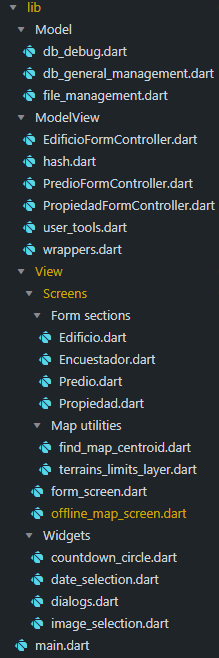
\includegraphics[scale=0.5]{Graphics/Capitulo 3/estructura_del_codigo.png}
    \caption{Estructura del código.} % Título de la figura
    \label{fig:figura14}
\end{figure}

En la figura anterior (Ver figura \ref{fig:figura14})se pueden apreciar las diferentes capas de la arquitectura MVVM bien definidas,
representadas por las carpetas "Model", "View" y "ViewModel" que contienen la parte del código relacionada con la capa de arquitectura
que su nombre indica:\\\\
\textbf{Model}\label{item:Model}\\
Aquí se encuentra la capa que abarca los datos y el acceso a ellos. Se hace uso de la librería sqflite \cite{sqflite} como mediador de comunicación
con bases de datos SQLite. Se encierra el modelo de datos en una jerarquía de clases reutilizable y expandible que tiene como padre la clase abstracta \textbf{InventarioDbTable},
de la cuál las clases que representan las tablas del modelo de datos del problema heredan, obligándoles a implementar propiedades y métodos que proporcionarán
el formato de los datos que requiere sqflite para insertar en sus tablas correspondientes. Estas clases asociadas a las tablas de la Base de Datos
son \textbf{Predio}, \textbf{Edificio} y \textbf{Propiedad}.
\\\\
\textbf{View}\\
El componente Vista está dividido en dos partes, las pantallas o "Screens" y los "Widgets"
\footnote{Los widgets son básicamente componentes de Flutter utilizados para crear la interfaz de usuario de
    la aplicación}.
Existen solo dos pantallas en este caso, la pantalla del mapa sin conexión, que es donde se hace uso de las librerías flutter\_map y flutter\_map\_mbtiles para
obtener el componente que renderiza el mapa a partir de un archivo con formato/extensión ".mbtiles", y la pantalla del formulario, donde se hace uso de la gran
cantidad de Widgets predefinidos que posee Flutter para los diversos campos de los subformularios. Además se definen subdirectorios para separar componentes que se
usan en ambas pantallas. Las partes que se usan para conformar la pantalla del formulario se encuentran dentro del subdirectorio \textbf{Form Sections} y son los
subformularios Predio, Edificio y Propiedad, que usan individualmente componentes/widgets de Flutter para los campos que se asocian con los datos de cada una de
las tablas que representan. Al mismo tiempo, la funcionalidad que se declara dentro del subdirectorio \textbf{Map utilities} es la declaración de un widget
que representa una capa de delimitaciones, el cuál se encarga de filtrar los polígonos que representan predios y calcular los centroides y pintarlos\\
Por otra parte, los Widgets que se definen son para el uso mayormente en la pantalla del formulario. Algunos de ellos son campos de formulario personalizados que
ofrecen una validación y son reactivos de acuerdo a lo que se necesita. Estos son los campos de fecha e imagen, además de algunos widgets que ayudan con el flujo
de procesos de la interfaz visual.
\\\\
\textbf{ModelView}\\
En este componente de la arquitectura está ubicado mayormente el estado de las variables de los formularios y la validación de los mismos. Los formularios se encargan
desde el componente Vista de mantener los datos de su controlador correspondiente actualizados a medida que cambian según la actividad del usuario en la interfaz,
y al usuario presionar en un boton de Guardar, el controlador correspondiente del componente ModelView se encarga de validar los datos, enviárselos al componente Modelo
para que los guarde en la base de datos, y luego de eso, haciendo uso del propicio patrón de utilización de funciones de callback\footnote{Funcion de callback es una
    forma de ejecutar una función en un punto del código deseado confiándole dicha función a un método u objeto pasándola como parámetro} de Flutter, se actualiza la interfaz
visual en consecuencia. Cabe destacar que por motivos de organización cada subormulario tiene su propio controllador en la capa de ModelView.
\\
\section{Modelo de Base de Datos} \label{section:dataModel}
Dada la naturaleza del problema: desarrollo en Android, desconexión de internet; y la naturaleza de Flutter, se escogió trabajar con el sistema gestor de bases de datos SQLite,
que ofrece simplicidad y una buena integración con Flutter a través de la librería sqflite, que a pesar de ser desarrollada por la comunidad, es un paquete muy utilizado y
testeado en ambientes de desarrollo. Por otra parte, solo hay que enfocarse en el modelado de las entidades y relaciones presentes en el problema, ya que una vez construida
la base de datos localmente, esta se exporta como archivo y se consume por un servicio externo, el cuál está fuera del margen de esta tesis.\\
También es importante mencionar que se hizo una variación en el modelo de datos de la aplicación anterior, ya que existían conceptos redundantes que podían causar confusión y
falta de claridad, pensando en primera instancia en los propios encuestadores, que son los futuros usuarios que utilizarán la aplicación final. En el modelo anterior existían
cinco módulos los cuáles describen cada uno una entidad sobre la cuál recoger información, y la propia información a recoger. Los cinco módulos y las respectivas entidades sobre
las que recogían información eran:

\begin{table}[h!]
\centering
\caption{Módulos comprendidos en la aplicación y modelo de datos anteriores}
\label{tab:modulosAnteriores} % Etiqueta para referenciar la tabla más adelante
\begin{tabular}{|r|l|}
    \toprule
    \textbf{Módulo}                     & \textbf{Entidad que encuesta}                      \\
    \midrule
    Terreno                             & Información sobre el Predio                        \\
    Construcción                        & Información sobre los edificios del Predio         \\
    Medidores Eléctricos                & Información sobre los edificios del Predio         \\
    Edificación                         & Información sobre los edificios del Predio         \\
    Uso de Suelo y Patentes Comerciales & Información sobre las propiedades de cada Edificio \\
    \bottomrule % Línea horizontal inferior (requiere booktabs)
\end{tabular}
\end {table}
Por ende, como se puede observar, existían 3 módulos de datos referenciando a la misma entidad, Edificio, por lo que se decidió factorizar estos módulos, agrupándolos en
\textbf{Predio}, \textbf{Edificio}, \textbf{Propiedad} y \textbf{Encuestador}.
Luego, la base de datos que modela el problema es bastante simple; en la figura \ref{fig:figura15} se muestra el diagrama Entidad-Relación del modelo de Datos:
\pagebreak
\begin{figure}[h]
    \centering
    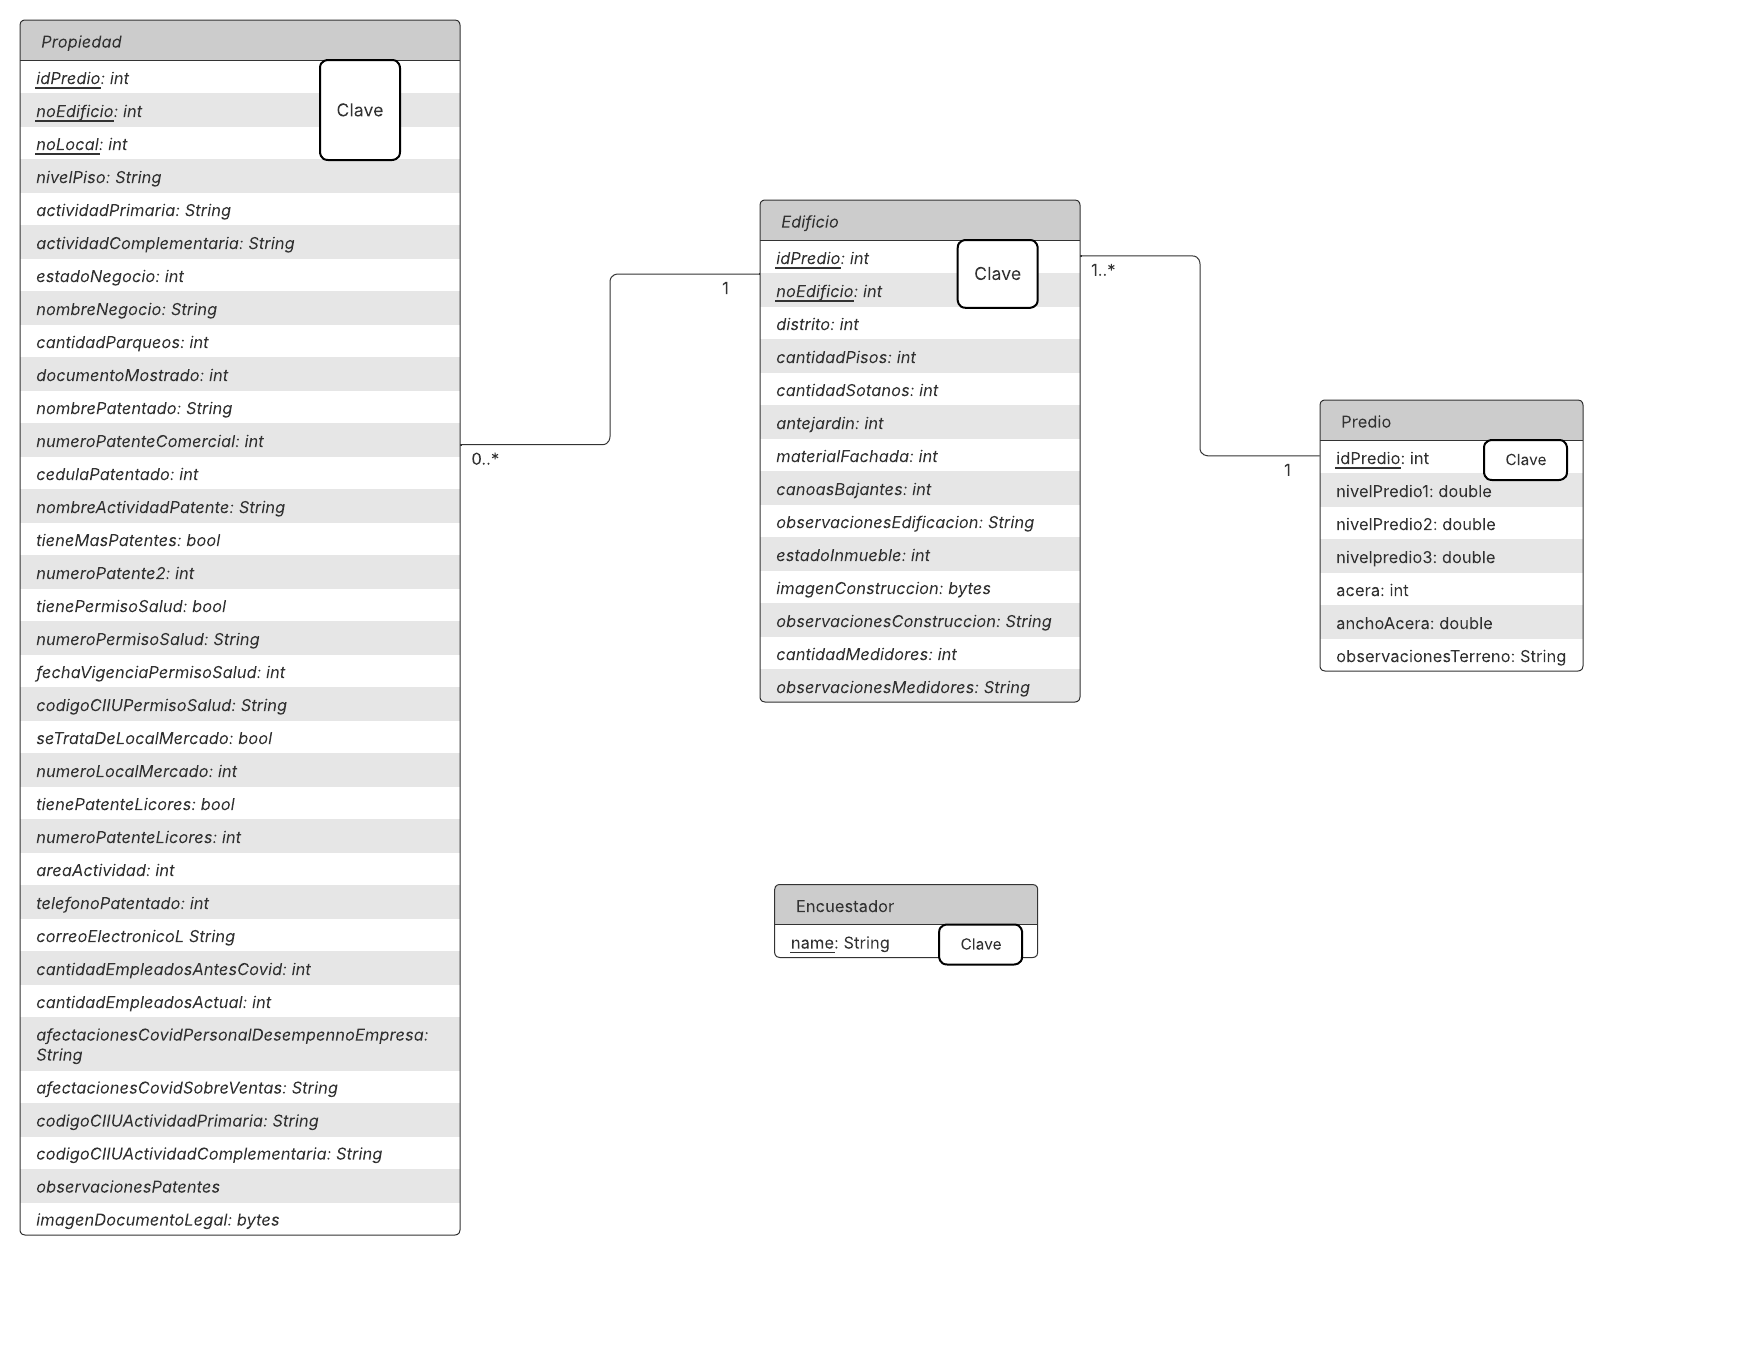
\includegraphics[scale=0.5]{Graphics/Capitulo 3/DiagramaER.png}
    \caption{Diagrama Entidad-Realción del modelo de datos.} % Título de la figura
    \label{fig:figura15}
\end{figure}
Cabe destacar que por motivos de optimización, en los campos de selección de una lista fija de valores como por ejemplo lo es el caso de "materialFachada" en la entidad Edificio, se almacena solo un valor entero que representa el índice de
la lista asociado con el valor que representa. Por ejemplo en este caso si el edificio que se está encuestando tiene un material de fachada Prefabricado, como en la lista de posibles materiales en la fachada, este valor es asociado con el índice 2,
pues ese sería el valor que tomaría este campo, en lugar de almacenar el texto completo "Prefabricado". Tener en cuenta también que no siempre los índices que correponden al valor siguen una secuencia, por ejemplo en el propio campo de materialFachada,
se tiene el valor 'No visible' cuyo índice asociado sería 999, teniendo esta lista solamente 8 elementos. En cada campo de selección se especificará la lista de valores con sus índices numéricos asociados.
\subsection{Predio}
En el modelo de datos, \textbf{Predio} es la única entidad fuerte, o sea, la existencia de un predio no depende de la existencia de ninguna otra entidad del modelo. Estos son los campos/variables que incluye una tupla de Predio:\\\\
\underline{idPredio}: Campo de tipo entero de 10 cifras. LLave primaria de la entidad \textbf{Predio}. Es el número de localización del predio, el cuál es único así que puede usarse como identificador.\\
\underline{nivelPredio1}, \underline{nivelPredio2} y \underline{nivelPredio3}: Campos numéricos, aceptan decimales, los cuáles se refieren a "la
diferencia de altura del acceso principal del edificio al punto de intersección entre la acera y el vértice"\\
\underline{acera}: Campo de tipo entero que dice el estado de la acera de un predio. Representa el índice de la opción que se escoja de la siguiente lista de opciones: [0: 'No existe', 1: 'Bueno', 2: 'Regular', 3: 'Malo']. Por ejemplo,
si este campo tiene valor 1 en un predio, significa que el estado de la acera de ese predio es \textbf{bueno}\\
\underline{anchoAcera}: Campo numérico que acepta decimales. Representa el ancho de acera que hay frente al predio.\\
\underline{observacionesTerreno}: Texto describiendo las observaciones hechas por el encuestador sobre el terreno del predio.\\\\
\subsection{Edificio}
Edificio es una entidad débil, la cuál posee una relación de dependencia de identificación con la entidad Predio, o sea, que una tupla de Edificio depende de la existencia de una tupla de Predio.
Estos son los campos/variables en la entidad Edificio:\\\\
- \underline{idPredio}, \underline{noEdificio}: Llaves primarias, ambas de tipo entero. idPredio a su vez es clave foránea y apunta hacia la entidad Predio.\\
- \underline{distrito}: Campo de tipo entero. Representa el índice del distrito al cuál pertenece el edificio, de la lista de distritos siguiente: [1: 'Carmen', 2: 'Merced', 3: 'Hospital', 4: 'Catedral', 5: 'Zapote', 6: 'San Francisco', 7: 'Uruca', 8: 'Mata Redonda', 9: 'Pavas']\\
- \underline{cantidadPisos}: Campo de tipo entero. Cantidad de pisos del edificio.\\
- \underline{cantidadSotanos}: Campo de tipo entero. cantidad de pisos por debajo del nivel de la acera.\\
- \underline{antejardin}: Campo de tipo entero. Evalúa la existencia de al menos 1/3 de área verde en la zona del antejardín. Representa un índice asociado a la lista [0: 'No existe', 1: 'Si existe', 996: 'En construcción', 998: 'No aplica']\\
- \underline{materialFachada}: Campo de tipo entero. Evalúa el material predominante en la fachada del edificio. Representa el índice del material que le corresponde de la lista: [1: 'Bloques y Concreto', 2: 'Prefabricado', 3: 'Vidrio y Metal', 4: 'Ladrillo', 5: 'Madera', 6: 'Mixto', 998: 'No aplica', 999: 'No visible']\\
- \underline{canoasBajantes}: Campo de tipo entero. Asociado a un índice de la lista: [0: 'No existe', 1: 'Cumple', 2: 'No cumple', 998: 'No aplica']\\
- \underline{observacionesEdificacion}: Texto describiendo las observaciones acerca de la edificación.\\
- \underline{estadoInmueble}: Campo de tipo entero. Asociado a un índice de la lista: [1: "Óptimo", 2: "Muy Bueno", 3: "Bueno", 4: "Intermedio", 5: "Regular", 6: "Deficiente", 7: "Malo", 8: "Muy Malo", 9: "Demolición", 998: "No Aplica"]\\
- \underline{imagenConstruccion}: Campo de tipo bytes que almacena una imagen referente a la construcción del edificio.\\
- \underline{cantidadMedidores}: Campo de tipo entero. Catidad de medidores eléctricos en el edificio.\\
- \underline{observacionesMedidores}: Texto describiendo las observaciones acerca de los medidores del edificio.\\
- \underline{observacionesConstruccion}: Texto describiendo las observaciones acerca de la construcción del edificio.\\
\subsection{Propiedad}
Propiedad es una entidad débil también, la cuál tiene relación de dependencia de identificación con la entidad Edificio, y por ende, con la entidad Predio, es decir que una propiedad depende de la existencia de un edificio y por ende de un predio.
Aquí se verán campos de tipo booleanos, o sea de Verdadero o Falso, que permitirán la existencia de otros campos. Por ejemplo, si el campo booleano 'tienePatenteLicores' está en falso, el campo 'numeroPatenteLicores' no se podrá rellenar. En el
caso del campo booleano 'tienePermisoSalud', tres campos dependen de su valor para ser rellenados o no. También existen campos de selección múltiple, los cuáles serán almacenados en un campo de tipo texto, que incluya los valores de la selección
separados por coma(","). Además, especificar que el campo de fecha 'fechaVigenciaPermisoSalud' en el formulario se tendrá la posibilidad de escoger desde un calendario y se verá la fecha en un formato bien definido, pero al almacenarse en la
base de datos, este será recogido como un número entero, que tendrá el formato 'AAAAMMDD'; y por último, también existen campos inhabilitados, o sea, que no podrán ser rellenados por los encuestadores. Estos campos se dejarán en la base de datos
para que sea posible añadirlo luego fácilmente por la entidad encargada en caso de querer hacerlo. \\
- \underline{idPredio}, \underline{noEdificio}, \underline{noLocal}:
- \underline{nivelPiso}:  Campo de tipo texto, en el que se debe anotar el número de piso en donde se encuentra localizada la actividad. Si es más de un piso, deberá anotarse el
rango de los pisos en que está localizado, ejemplo, 1-7 (piso 1 al piso 7), o si la actividad también se desarrolla en un sótano, entonces seria, por ejemplo -1-4 (sótano 1 al piso 4). \\
- \underline{actividadPrimaria}: Campo de tipo texto, en donde se anotará la actividad principal encontrada. \\
- \underline{actividadComplementaria}:  Campo de tipo texto, en donde se anotará la actividad menos predominante.\\
- \underline{estadoNegocio}: Campo de tipo texto que se basa en una selección múltiple que evaluará la situación actual del negocio. La lista de opciones a escoger es: ['En operación', 'Cierre temporal', 'Desocupado con Rótulo SE ALQUILA', 'Cierre total', 'Ha modificado la actividad autorizada(EXPRESS u otra actividad)].\\
- \underline{nombreNegocio}:  Campo de tipo texto, en el cual se anotará el nombre de fantasía del negocio, ubicado en la publicidad (rotulo, vallas, ventanería, etc.). \\
- \underline{cantidadParqueos}: Campo numérico, en donde se anotará la cantidad de espacios de parqueos observada con que cuenta el inmueble. \\
- \underline{documentoMostrado}: Campo de tipo entero. Representa el índice que asocia el tipo de documento presentado que represente la patente de la actividad de la siguiente lista: [1: 'Certificado Patente', 2: 'Recibo al día(Menos de dos meses de atraso)', 3: 'Recibo atrasado(Con más de dos meses de atraso)', 4: 'Certificado Trámite "CT". Indicar el número', 5: 'No muestra documentos de patente']. \\
- \underline{nombrePatentado}: Campo de tipo texto, en el cual se deberá anotar el nombre de quien está en la patente comercial del negocio. \\
- \underline{numeroPatenteComercial}: Campo de tipo entero. Número de patente comercial o código específico en casos señalados puntuales. \\
- \underline{cedulaPatentado}: Campo de tipo entero, en el cual se anotará el número de cedula que se muestra en el certificado o recibo de la patente. \\
- \underline{nombreActividadPatente}: Campo de tipo texto en donde se anotará la actividad que aparece en la patente en un lugar específico. \\
- \underline{tieneMasPatentes}: Campo de tipo booleano. \\
- \underline{numeroPatente\_2}: Campo de tipo entero. Este campo estará presente solo si el campo 'tieneMasPatentes' está marcado. \\
- \underline{tienePermisoSalud}: Campo de tipo booleano. \\
- \underline{numeroPermisoSalud}: Campo de tipo entero. Este campo estará presente solo si el campo 'tienePermisoSalud' está marcado. \\
- \underline{fechaVigenciaPermisoSalud}: Campo de tipo entero que almacena la fecha en el formato 'AAAAMMDD'. Este campo estará presente solo si el campo 'tienePermisoSalud' está marcado. \\
- \underline{codigoCIIUPermisoSalud}: Campo de tipo texto. Código CIIU\footnote{El Código CIIU, o Clasificación Industrial Internacional Uniforme, es un sistema de clasificación de actividades económicas a nivel mundial. Se utiliza para agrupar y categorizar las diferentes actividades que realizan las empresas y personas naturales, facilitando así la recopilación y análisis de datos estadísticos a nivel nacional e internacional} del permiso de salud: código que aparece en el permiso de salud de la actividad económica que se desempeña. Este campo estará presente solo si el campo 'tienePermisoSalud' está marcado. \\
- \underline{seTrataDeLocalMercado}: Campo de tipo booleano. \\
- \underline{numeroLocalMercado}: Campo de tipo entero. Este campo estará presente solo si el campo 'seTrataDeLocalMercado' está marcado. \\
- \underline{tienePatenteLicores}: Campo de tipo booleano \\
- \underline{numeroPatenteLicores}: Campo de tipo entero. Este campo estará presente solo si el campo 'tienePatenteLicores' está marcado. \\
- \underline{areaActividad}: Campo de tipo entero. Representa el índice asociado a una de las opciones de la siguiente lista: [1: 'Menos de 50m²', 2: '51 a 100m²', 3: '101 a 200m²', 4: '200 a 400m²', 5: '400 a 1000m²', 6: 'Más de 1000m²', 998: 'No aplica', 999: 'No visible']. \\
- \underline{telefonoPatentado}: Campo de tipo entero, con el número telefónico del propietario del inmueble. \\
- \underline{correoElectronico}: Campo de tipo texto. Correo del propietario. \\
- \underline{cantidadEmpleadosAntesCovid}: Campo de tipo entero. \\
- \underline{cantidadEmpleadosActual}: Campo de tipo entero. \\
- \underline{afectacionesCovidPersonalDesempennoEmpresa}: Campo de texto. Es conformado por un campo de selección múltiple de entre las opciones de la siguiente lista: ['Despido de empleados', 'Reducción jornada laboral', 'Suspensión del contrato laboral', 'Se adelantaron vacaciones', 'Se empezó a trabajar por turnos', 'Se aumentaron las jornadas', 'Se implementó modalidad de teletrabajo']. \\
- \underline{afectacionesCovidSobreVentas}: Campo de texto. Es conformado por un campo de selección múltiple de entre las opciones de la siguiente lista: ['Ingresó "0" ante la afectación de una orden sanitaria', 'Reducción de los ingresos entre un 50-90\%', 'Reducción de los ingresos entre un 20-50\%', 'Se mantuvieron dentro de lo esperado', 'Aumentaron', 'Ninguna', 'NS-NR'] \\
- \underline{codigoCIIUActividadPrimaria}: Campo de tipo texto. Inhabilitado. \\
- \underline{codigoCIIUActividadComplementaria}: Campo de tipo texto. Inhabilitado \\
- \underline{observacionesPatentes}: Texto describiendo las observaciones acerca de la construcción del edificio. \\
- \underline{imagenDocumentoLegal}: Campo de tipo bytes que almacena una imagen que capture el documento legal mostrado por la entidad. \\

\section{Tecnologías y librerías utilizadas}
\subsection{Dart}
Como base decisiva, tanto para la fácil integración de la arquitectura pensada, como para la organización y productividad a la hora de depurar el código del proyecto,
es imprescindible mencionar a Dart, un lenguaje orientado a objetos, fuertemente tipado aunque con inferencia de tipos, basado en clases, con Garbage Collector
\footnote{El Garbage Collector es un sistema automatizado que libera la memoria que ya no está siendo utilizada por un programa}
y una sintaxis al estilo C, que puede compilar tanto a código nativo como a JavaScript. Admite interfaces, mixins, clases abstractas, genericidad, entre otras maravillosas cualidades. \cite{dartOficial}
\subsection{Paquete geolocator}
Este paqute se utilizó para la facilitación de la funcionalidad de obtener la geolocalización en tiempo real del dispositivo Android sobre el que está corriendo la aplicación.
Este paquete ofrece una gran facilidad en el manejo de los permisos de geolocalización y clases y métodos bastante útiles para el trabajo con posiciones geográficas.
\subsection{Paquete latlong2}
LatLong es un paquete que incorpora Geodesia y Cálculos Geográficos para Dart,
proporciona una biblioteca liviana para el uso de proyecciones LatLong, o sea latitud y
la longitud, las unidades que representan las coordenadas en el sistema de coordenadas
geográficas. \cite{latlong2}
\subsection{Paquetes file\_picker e image\_picker}
File Picker es un paquete para iOS y Android que permite usar el explorador de archivos nativo para seleccionar uno o varios archivos con soporte de filtrado de extensiones,
de igual manera Image Picker es un plugin de Flutter que permite seleccionar archivos,
en este caso imágenes de la biblioteca de imágenes y tomar nuevas fotos con la cámara.

\subsection{Paquete permission\_handler}
Este paquete fue clave en el manejo de permisos de escritura de archivos. La aplicación para iniciarse, por comodidad y organización debe obtener los permisos de manejo y escritura sobre el sistema de archivos
del sistema de archivos del dispositivo, y en Android, los permisos de escritura en las últimas versiones han cambiado mucho, volviéndose una odisea tener en cuenta el tipo de permiso que se debe pedir
según la versión de sdk o de sistema operativo que tenga el dispositivo. Este paquete es bastante útil para el manejo de permisos, incluyendo incluso funciones que redireccionan al usuario hacia los ajustes del
dispositivo para que concedan el permiso, en caso que no haya otra opción.
\subsection{Paquete image}
En SQLite, el almacenamiento de imágenes tiene un problema, y es que el tamaño de archivos multimedia en campos "BLOB"
\footnote{Un campo BLOB, o Objeto Binario Grande, es un tipo de campo en bases de datos utilizado para almacenar datos binarios de gran tamaño, como imágenes, audio, video o documentos}
tiene un límite de tamaño. Se sugiere almacenar en campos BLOB archivos de no más de 5mb. Por esta razón fue necesario usar el paquete image\cite{image} para procesar y comprimir las imágenes mayores de 1.8mb, que ya sería un tamaño no tan prudente
para un archivo a ser almacenado en un campo BLOB de SQLite.
\section{Detalles de implementación}
En esta subsección se explicará de cara al desarrollador, la implementación de cada uno de los elementos visuales de los subformularios en la capa o componente View, y la relación con sus controladores en la capa o componente ModelView. También se explicarán .\\\\
\subsection{Subformularios}
Como ya se mencionó, existen varios subformularios que integran la funcionalidad de Registro en la aplicación Inventario. Ellos son Predio, Edificio y Propiedad. Estos solo están integrados por la parte visual de sus respectivos campos, y una mínima implementación
de funciones pequeñas de validación de campos, como comprobaciones de nulidad, o si el valor que se introdujo en un campo es entero, o verificar la cantidad de cifras de un número no es correcta. En la siguiente figura se presenta un fragmento del código del subformulario
Predio donde se puede ver parte de la implementación de algunos campos del mismo(ver Figura \ref{fig:figura16}).

\begin{figure}[h]
    \centering
    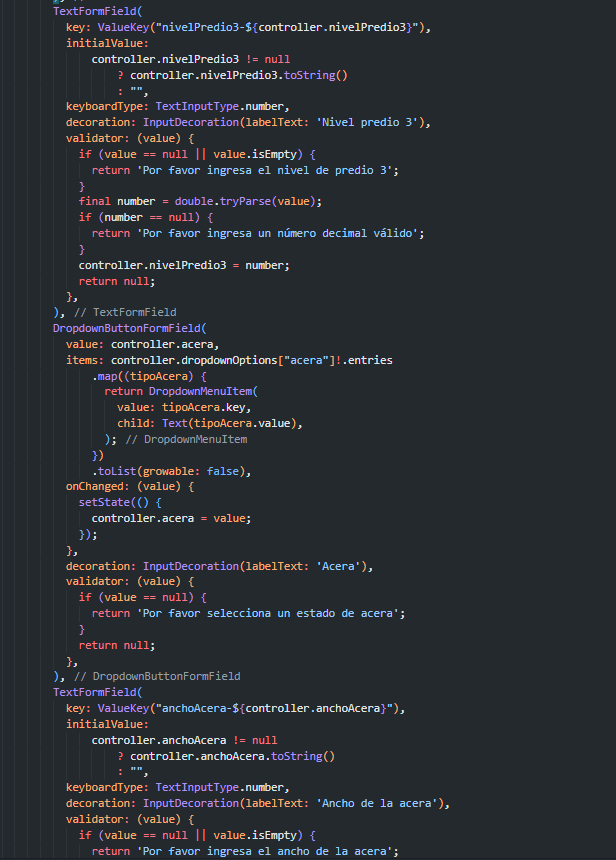
\includegraphics[scale=0.5]{Graphics/Capitulo 3/formulario_predio.png}
    \caption{Fragmento de la implementación del subformulario Predio} % Título de la figura
    \label{fig:figura16}
\end{figure}

Como ya se analizó en el epígrafe \ref{section:dataModel}, se tienen varios predios, donde cada uno de estos predios puede contener varios
edificios, y cada uno de estos edificios puede contener varias propiedades. Luego para agregar un edificio a la base de datos se debe prefijar un predio
y para agregar una propiedad a la base de datos se debe prefijar un predio y un edificio dentro de ese predio.\\
A nivel global, durante toda la ejecución, se mantiene un objeto de manera estática que tiene tres valores enteros, que también pueden ser null.
Esta variable se llama 'formGlobalStatusWrapper' o simplemente 'formGlobalStatus', y los 3 valores enteros que guarda son los identificadores del predio,
el edificio y la propiedad que se estén editando. Por ejemplo, si:
\begin{itemize}
    \item formGlobalStatus['idPredio'] = 1000000001, formGlobalStatus['noEdificio'] = null y formGlobalStatus['noLocal'] = null: Significa que se está trabajando sobre el
          predio con ese número de localización, pero no se está editando ningún edificio existente, y por ende ninguna propiedad.
    \item formGlobalStatus['idPredio'] = 1000000001, formGlobalStatus['noEdificio'] = 1 y formGlobalStatus['noLocal'] = null: Significa que se está trabajando sobre el edificio
          número 1 del predio 1000000001
    \item formGlobalStatus['idPredio'] = 1000000001, formGlobalStatus['noEdificio'] = 1 y formGlobalStatus['noLocal'] = 34: Significa que se está trabajando sobre la propiedad 34 del edificio
          número 1 del predio 1000000001.
\end{itemize}
Por lo tanto estas tres variables van a definir básicamente sobre qué entidades se están trabajando. Ahora, haciendo uso del patrón de utilización de funciones callback, se realizó un sistema de
eventos, donde se permite la posibilidad de, dentro de esta estructura 'formGlobalStatus' suscribirse a los eventos de asignación de las variables formGlobalStatus['idPredio'], formGlobalStatus['noEdificio'] y formGlobalStatus['noLocal']
a funciones que, según qué predio, edificio, o propiedad esté activa, renderizar el formulario en consecuencia.
\subsection{Reactividad de los formularios}
Luego, cada subformulario, tiene su propio controlador, declarado como una variable. El controlador,
que forma parte de la capa ModelView, estaría abstraído de lo que ocurre con la interfaz del formulario. El controlador simplemente guardaría el estado
de las variables. Cada formulario, al sí tener control de su estado, puede acceder a él para en base a si hay algún cambio, renderizar su interfaz visual en consecuencia.
Esto se logra haciendo uso del principio de llaves de widgets en Flutter, que plantea que si una llave de un widget cambia, este widget deberá ser renderizado nuevamente
Por ejemplo, en la Figura \ref{fig:figura16} podemos observar como cada uno de los campos de Predio, obtiene el valor del estado de su variable, y lo establece como
valor inicial del campo y también lo establece como llave a ese campo, diciéndole a Flutter que cuando este valor cambie, debe cambiar también la interfaz visual. Esto provoca que
al cambiarse el estado global de la aplicación(variable formGlobalStatus), se desencandenen una serie de acciones al intentar renderizar los 3 subformularios:
\begin{enumerate}
    \item Cada subformulario inicializa su controlador
    \item El Controlador de Predio le pide al Modelo que busque el predio con número de localización igual a formGlobalStatus['idPredio']
    \item El Controlador de Edificio le pide al Modelo que busque todos los Edificios que tienen como número de localización: formGlobalStatus['idPredio'] para asi tenerlos listos para la UI.
    \item El Controlador de Edificio, en caso de que formGlobalStatus['noEdificio] != null, inicializa su estado con los datos del edificio que esté dentro del predio con número de localización igual a
          formGlobalStatus['idPredio'] y con número de Edificio igual a formGlobalStatus['noEdificio'].
    \item $\cdots$
    \item El View de Edificio, al comenzar a renderizarse, accede al estado de su Controlador y autorrellena el formulario en caso de tener variables con valores. Además muestra la lista de edificios del predio en el tope del formulario como elementos visuales para ser seleccionados
    \item $\cdots$
\end{enumerate}
El mismo proceso ocurre con Propiedad y su Controlador, pero esta vez chequeando la variable formGlobalStatus['noLocal'] y encontrando las propiedades que pertenezcan al edificio con número formGlobalStatus['noEdificio']\\
\subsection{Validación de formularios}
La validación de los formularios ocurre en los respectivos controladores, o sea, en la capa ModelView. El botón de la UI invoca la función del controlador 'validateForm', este al tener la llave del formulario del view,
invoca el método validate() y se validan todos los campos del formulario, si son válidos, se procede a ver si existe un caso de sobrescritura, o de añadir un edificio sobre un predio que aún no está en la Base de Datos, etc,
y en caso de no haber problemas, se le pasa la tupla al modelo en forma de clase y el modelo lo convierte en un Map<String, dynamic> y lo introduce en la base de datos, el Model responde al ModelView que si se pudo guardar la tupla,
por ende el ModelView le deja saber al View lo mismo, y este último le muestra un mensaje al usuario de confirmación de operación.
% \subsection{Restricciones y visibilidad de campos de los formularios}

\subsection{Exportación e importación de archivos}
La única forma de mostrar mapas sin conexión a Internet con Flutter(sin descarga inicial siquiera) es con la librería flutter\_map\_mbtiles, y esta lee los archivos de mapas en formato ".mbtiles" por lo que fue obligatorio el uso de este tipo de formato de archivo de mapa
sqlite. Luego, para la importación de capas de delimitaciones encima del mapa base, se escogió el formato gegojson por la claridad que ofrece, además de la cantidad de herramientas que existen hoy en día que crean polígonos
de una manera rápida y efectiva, además de la facilidad de lectura y extracción de datos, leyendo estos archivos como json con librerías built-in de Dart. Ya se expusieron las razones de por qué se escogió SQLite como sistema gestor de bases de datos.
Revisar el formato de entrada del las delimitaciones en archivos geojsonen a inicios de este capítulo(Ver \ref{item:importaciongeojson}) para su correcta importación
\subsection{Extensión del código}
En esta subsección se hablará un poco más de la capa Model y de como extender el modelo de datos en caso que se desee, ya que en realidad los datos son la característica principal de una aplicación de categoría SIG.
La capa Model esta compuesta por 3 archivos, 'db\_debug.dart', 'db\_general\_management.dart' y 'file\_management.dart', pero en realidad donde se concentra el diseño del modelo es en 'db\_general\_management.dart'. Se diseñó una jerarquía de clases con el objetivo de
entregar un proyecto expansible y reutilizable, la cual consta, como ya se explicó a grandes rasgos en\ref{item:Model}de una clase abstracta 'InventarioDbTable' que tiene la implementación de las operaciones de eliminación, actualización e inserción, basados en propiedades que debe
implementar o proveer toda clase que herede de 'InventarioDbTable'. Al crear una clase que hereda de InventarioDbTable, ya que los parámetros 'tableName' y 'primaryKeysWhere' son obligatorios, Dart exigirá que en el constructor de las clases herederas se llame al constructor de su padre
y provea estos dos parámetros mediante la palabra reservada de Dart 'super' y la invocación con los paréntesis, haciendo inclusión de dichos datos mediante el uso de los parámetros de nombre de Dart. Por otra parte, hay una propiedad o 'getter' y un método en la clase 'InventarioDbTable' que al
una clase heredar de esta clase abstracta, Dart te exigirá implementar en la clase heredera. El getter se llama 'primaryKeysWhereArgs' y el método se llama 'toMap()' y junto con los demás parámetros y la definición de la tabla en SQLite, se tiene todo lo necesario para que se ejecute automáticamente la inserción, actualización y eliminación sobre esta nueva tabla.
\\\\
\textbf{tableName}\\
Este parámetro es para establecer una conexión directa con la tabla que representa el modelo. Debe ser el nombre exacto de la tabla que se declare en sqlite.
\\\\
\textbf{toMap()}\\
Este método por convenio debe devolver un Map<String, dynamic> que contenga en sus 'keys' los nombres exactos de los campos de la tabla sqlite que se declaró y en los 'values', los valores asociados que deben ser del mismo tipo que sus campos respectivos declarados en la tabla sqlite asociada.
Este método se usa para la inserción y la actualización.
\\\\
\textbf{primaryKeysWhere} y \textbf{primaryKeysWhereArgs}\\
A la hora de hacer consultas con sqflite, estas se declaran de la forma:
\begin{mdframed}
    database.query(tableName, where: "idPredio = ? AND noEdificio = ?", whereArgs: [predio.idPredio, edificio.noEdificio]);
\end{mdframed}
El objetivo es entregar en este formato: String y List<dynamic> respectivamente las claves primarias de la nueva tabla. Para una idea más clara, en la figura \ref{} se tiene la implementación que
hace la clase 'Encuestador' del Modelo de la clase abstracta 'InventarioDbTable'
\\\\
\begin{figure}[h]
    \centering
    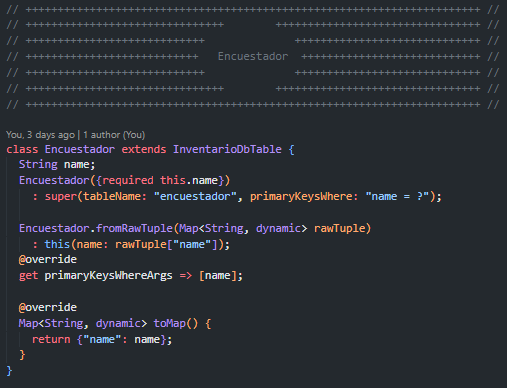
\includegraphics[]{Graphics/Capitulo 3/implementacion_InventarioDBTable.png}
    \caption{Implementación de la clase abstracta 'InventarioDbTable' por la clase 'Encuestador'}
    \label{fig:figura17}
\end{figure}


Completando esto y por supuesto la declaración de la tabla correspondiente en SQLite se tendrá una nueva entidad integrada en el Modelo de Datos
\\
% \\\\
% \section{Conclusiones del capítulo}
\chapter{Pruebas de funcionalidad}\label{chapter:implementation}
En este capítulo se realizan un conjunto de pruebas para demostrar el buen funcionamiento de las herramientas implementadas y así evidenciar el cumplimiento de los
objetivos planteados en este trabajo.
Las pruebas se realizaron en dos dispositivos Android físicos y uno emulado desde Android Studio para abarcar la mayor cantidad de casos posibles\\
Los dispositivos tienen las siguientes prestaciones:\\
\section{Prestaciones de los dispositivos sobre los que se ejecutaron las pruebas}
\subsection{LG VELVET Android 13 [Dispositivo físico]}
\begin{itemize}
    \item 5.7 Gb RAM
    \item CPU Octa-Core a una frecuencia promedio por núcleo de 1.925 GHz
\end{itemize}
\subsection{Samsung Galaxy S23 Ultra Android 14 [Dispositivo físico]}
\begin{itemize}
    \item 8.0 Gb RAM
    \item CPU Octa-Core a una frecuencia promedio por núcleo de 2.57 GHz
\end{itemize}

\subsection{Google Pixel 4 Android 10 [emulador]}
\begin{itemize}
    \item 2.0 Gb RAM
    \item CPU Quad-Core
\end{itemize}


\section{Importación de un mapa}
\begin{figure}[h]
    % \centering
    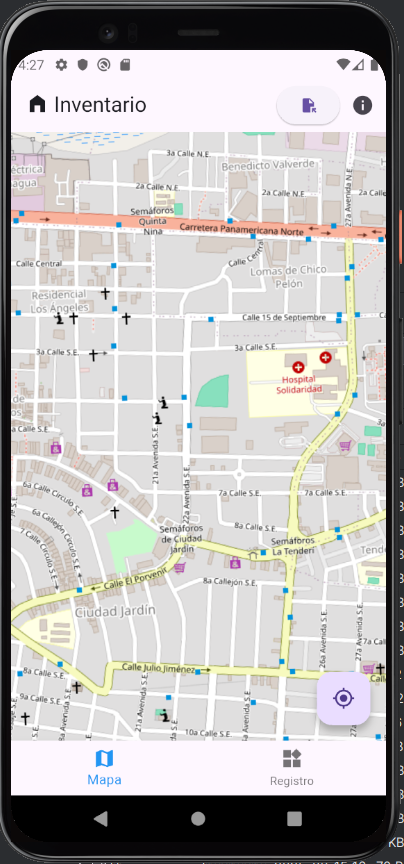
\includegraphics[width=0.3\textwidth]{Graphics/Capitulo 4/Pixel 4 [emulador]/4.2/1.png}
    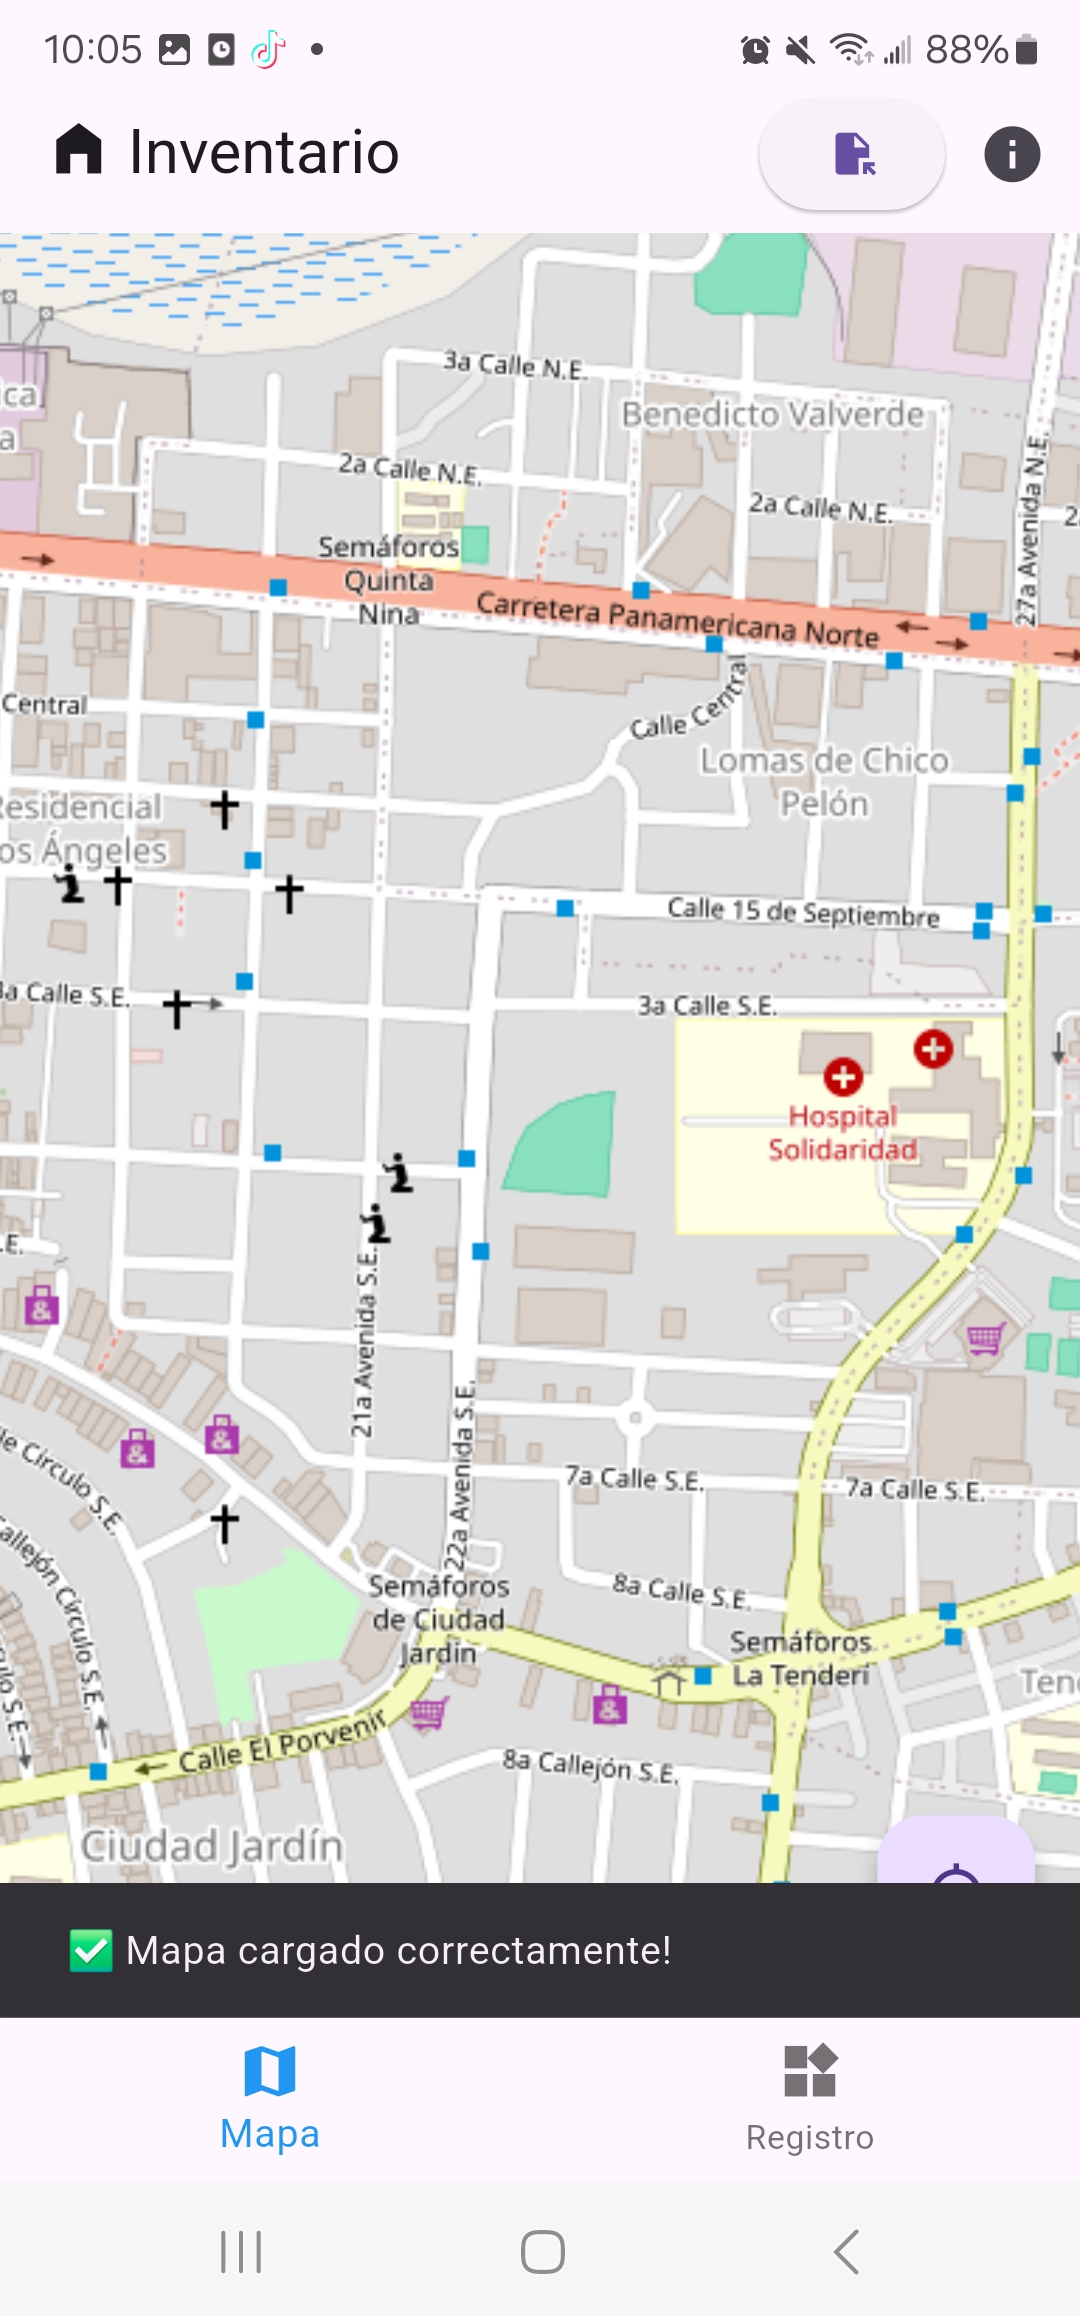
\includegraphics[width=0.3\textwidth]{Graphics/Capitulo 4/Galaxy S23 Ultra Android/4.2/3.jpg}
    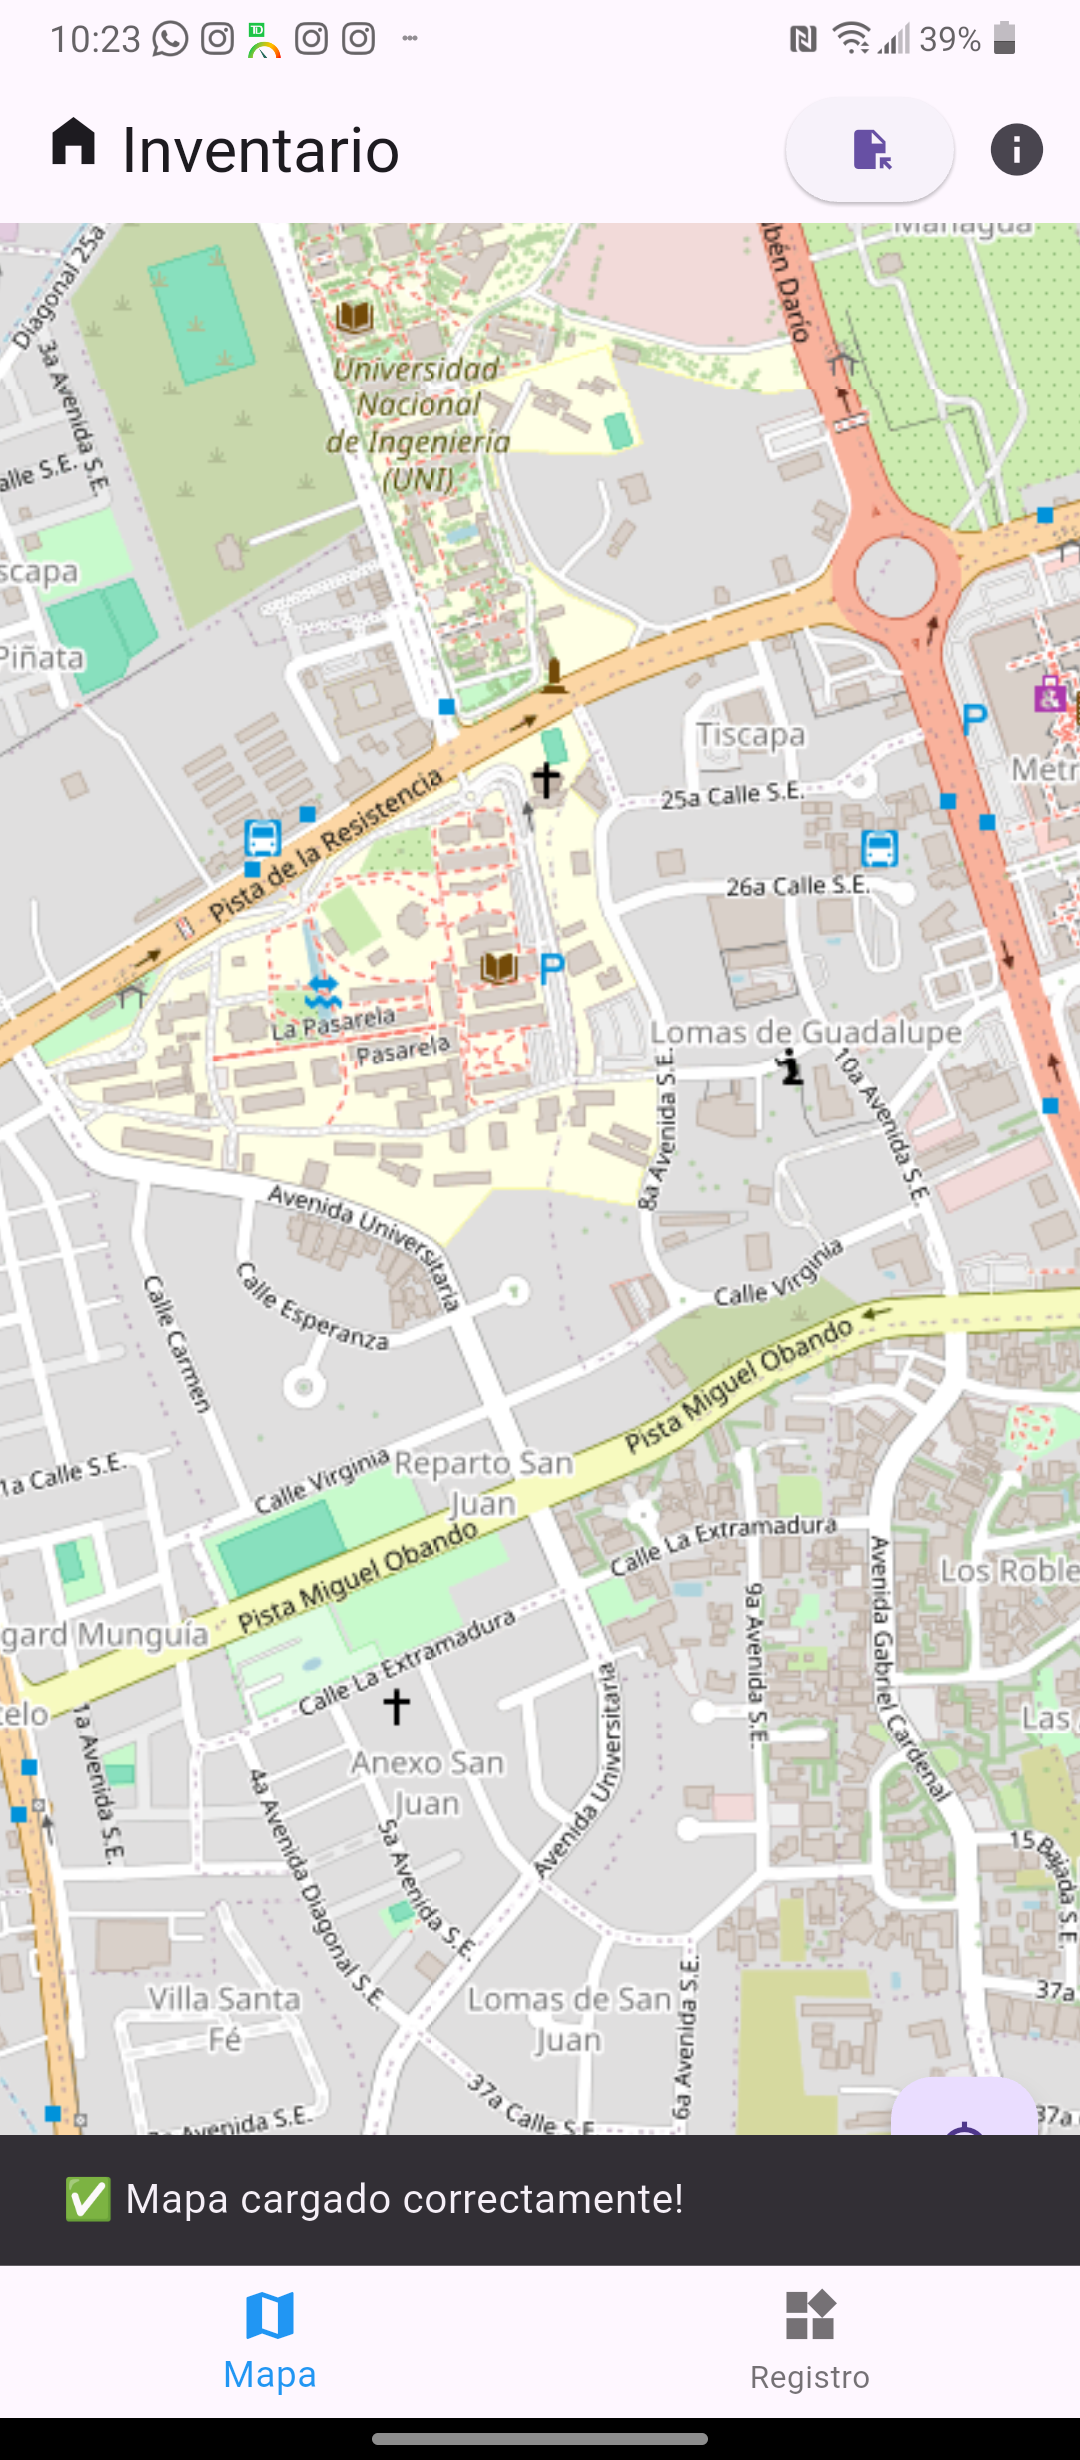
\includegraphics[width=0.3\textwidth]{Graphics/Capitulo 4/LG Android 13/4.2/2.png}
    \caption{Prueba de importacion de mapa}
    \label{fig:figura18}
\end{figure}
Esta constituye una prueba básica de las funcionalidades de la aplicación pero se debe tener en cuenta que también se está analizando compatibilidad
con versiones de Android antiguas como la 10 y esto es una prueba válida dada la inmensa cantidad de variaciones que se han hecho desde 2019(seis años atrás)
hasta la actualidad en actualizaciones del SO.

\pagebreak
\section{Importación de varias capas de delimitación, una de ellas con el formato de predios}
\begin{figure}[h]
    % \centering
    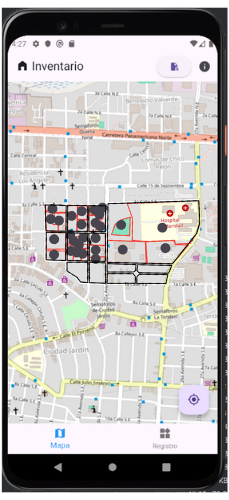
\includegraphics[width=0.3\textwidth]{Graphics/Capitulo 4/Pixel 4 [emulador]/4.3/1.png}
    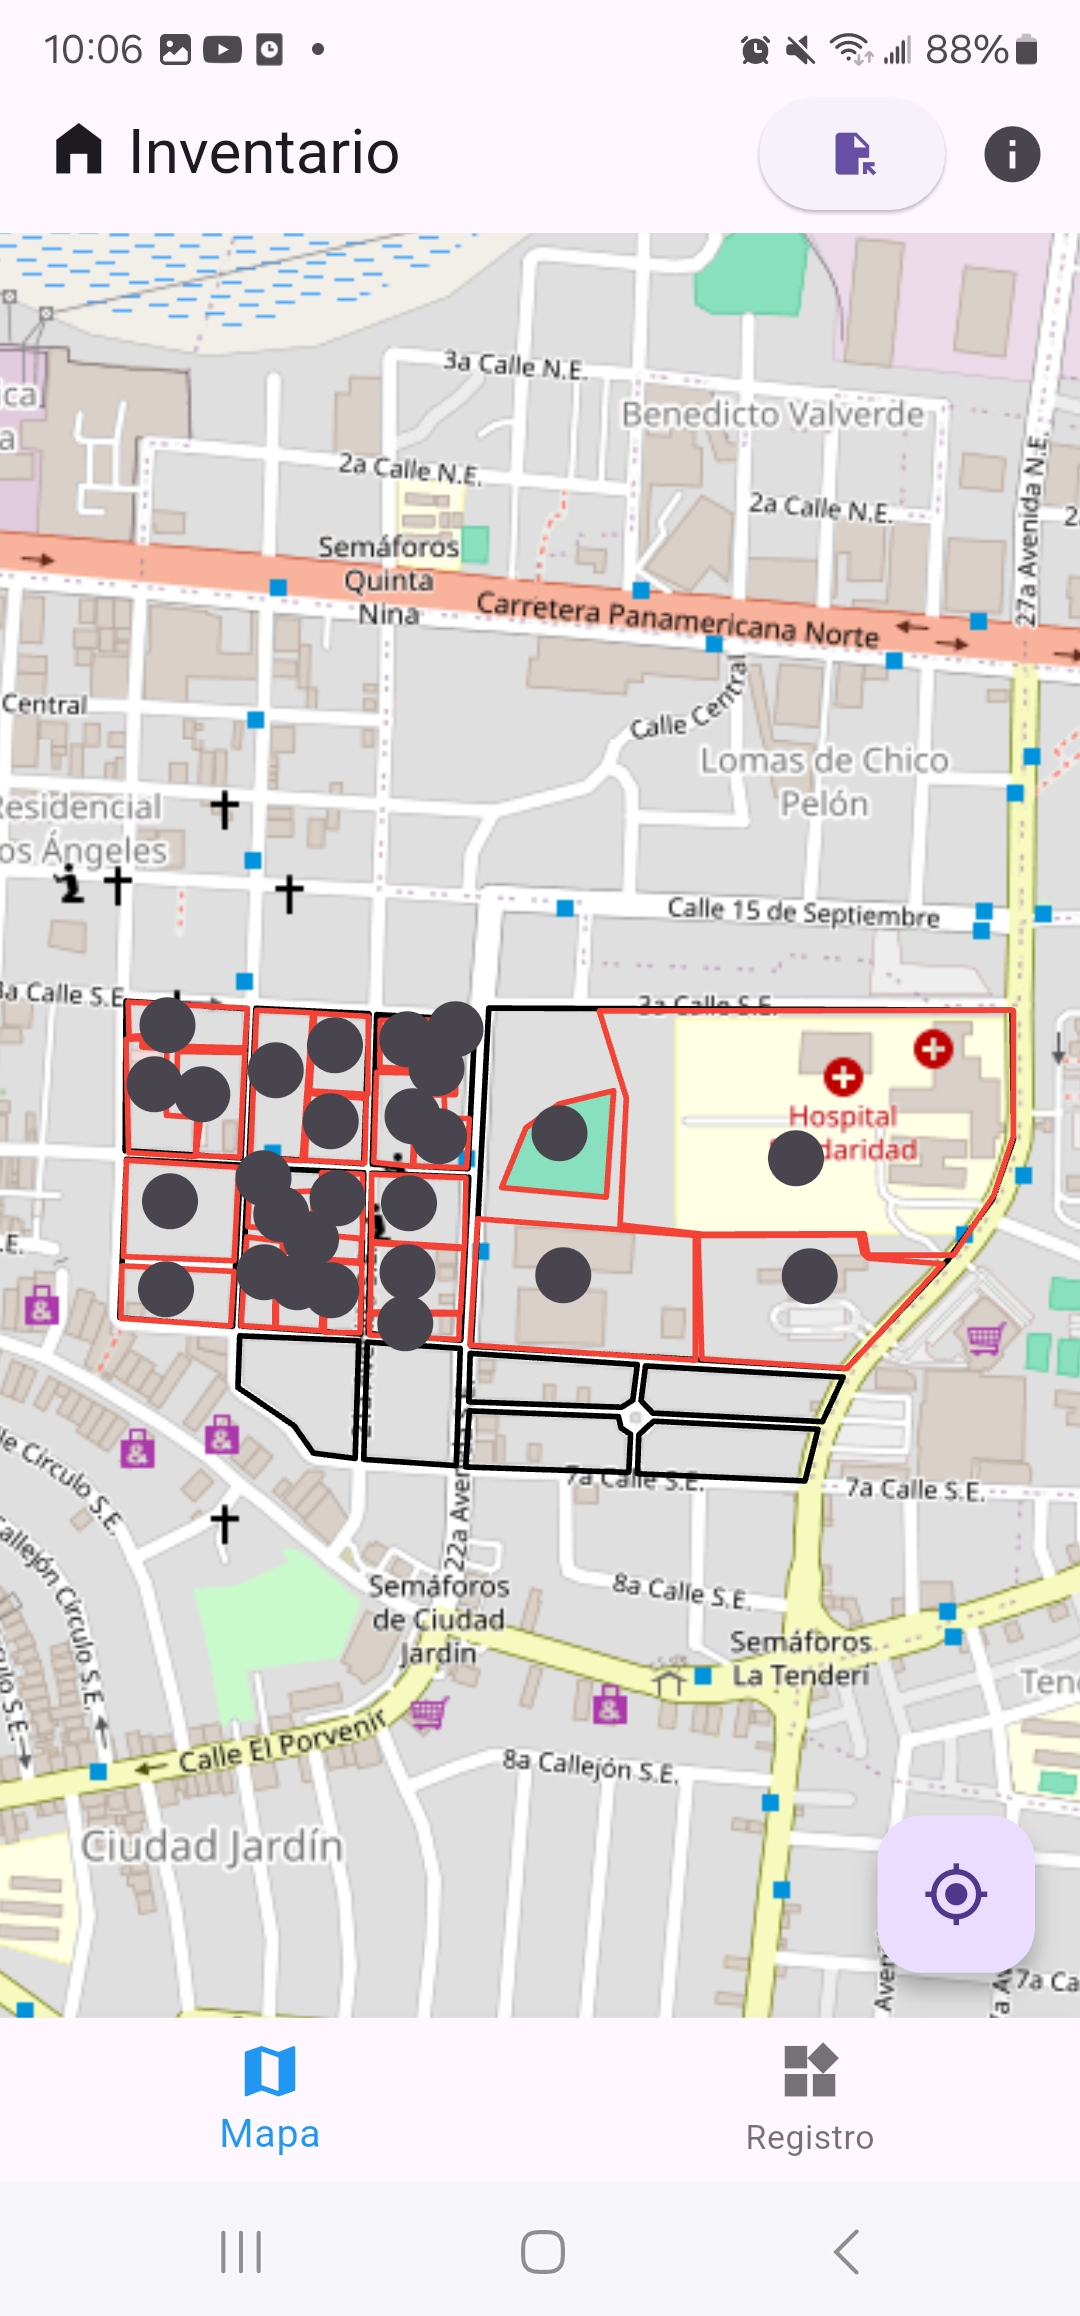
\includegraphics[width=0.3\textwidth]{Graphics/Capitulo 4/Galaxy S23 Ultra Android/4.3/4.jpg}
    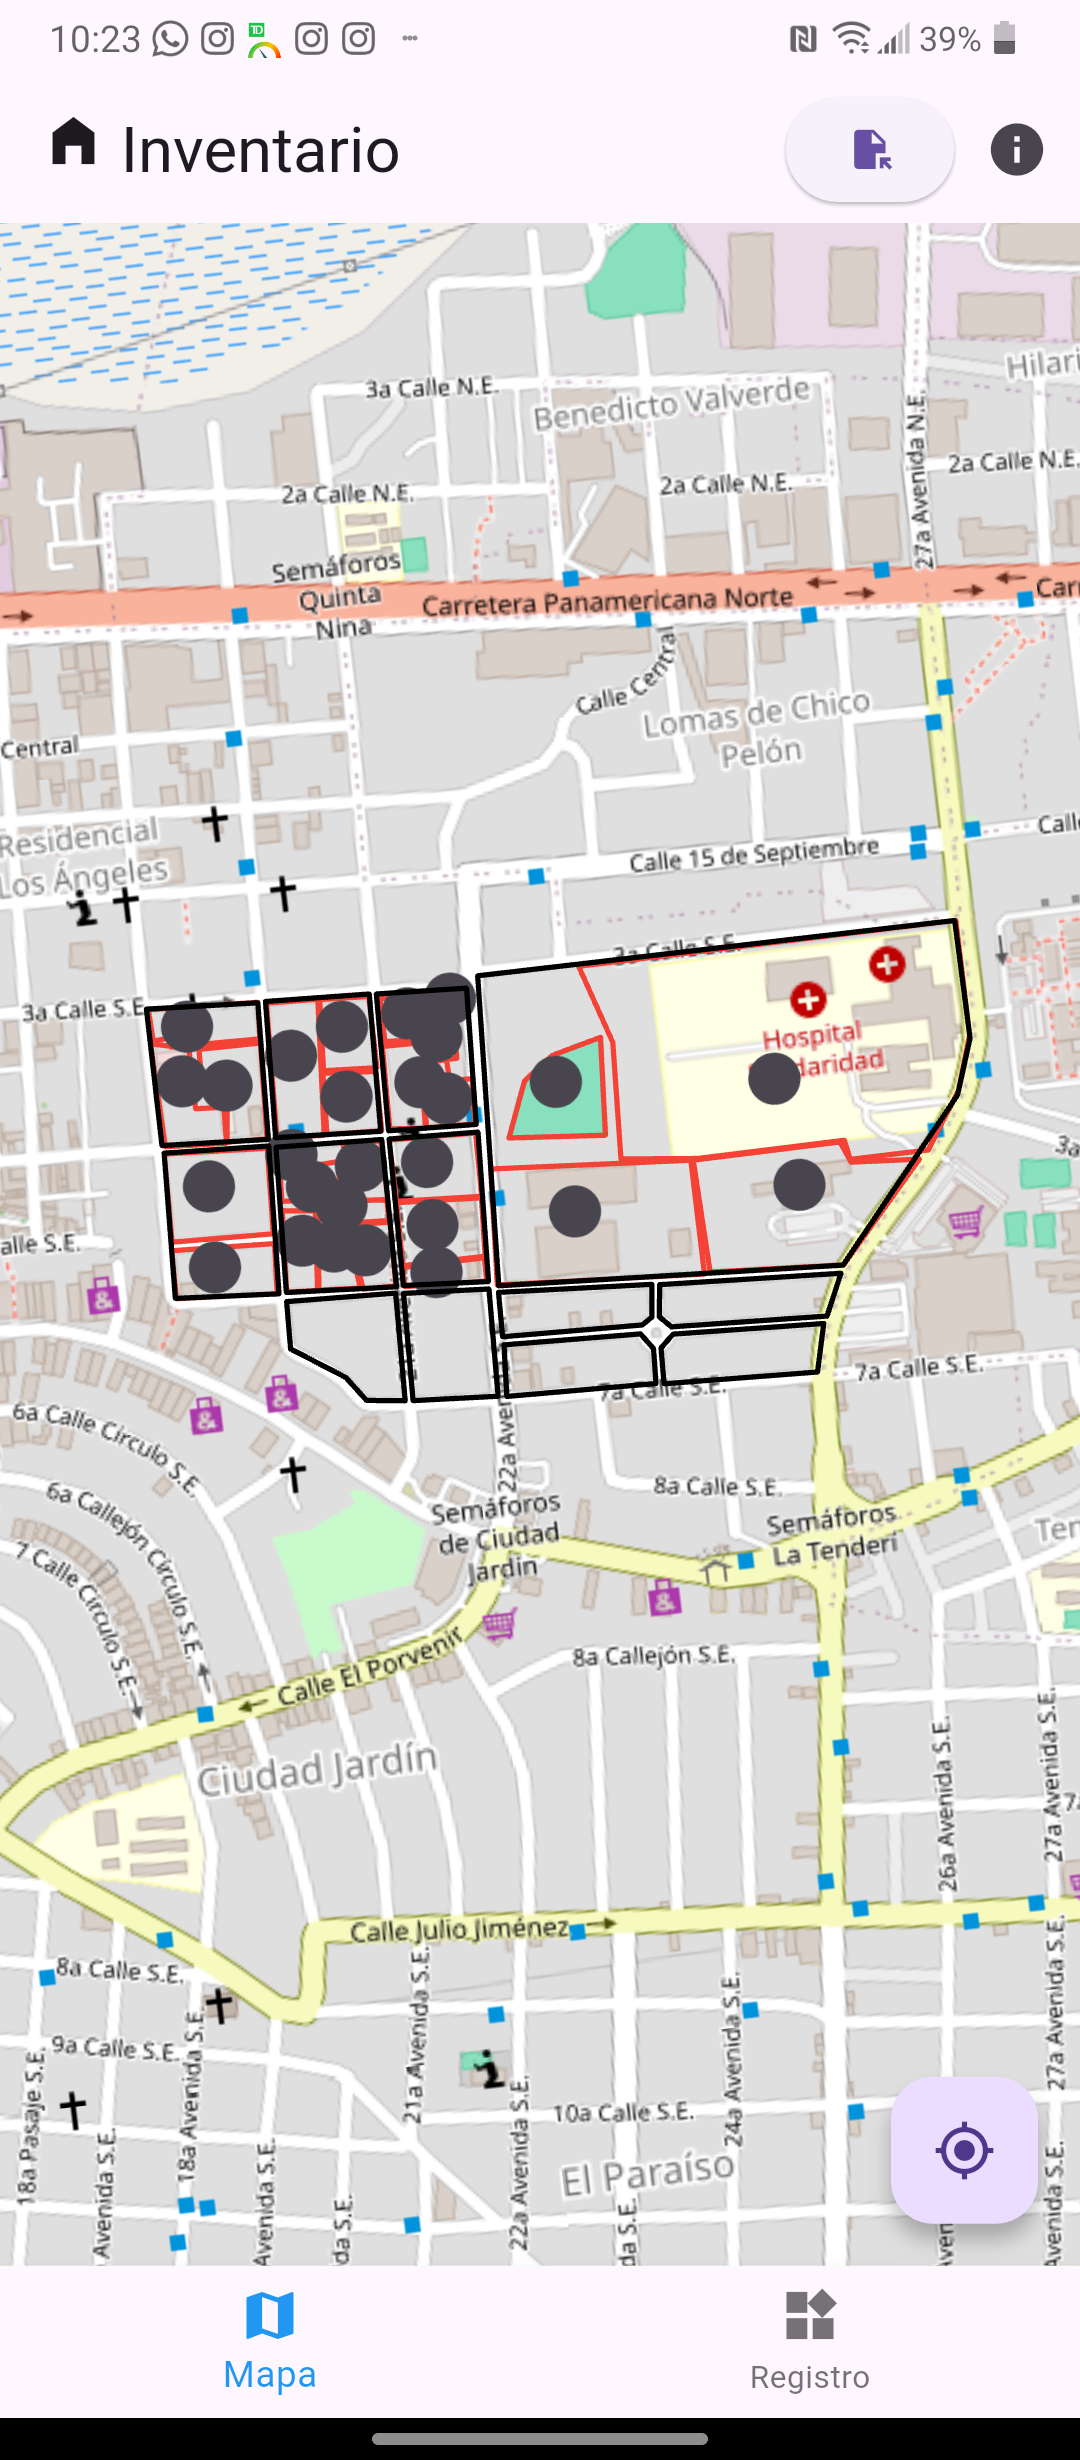
\includegraphics[width=0.3\textwidth]{Graphics/Capitulo 4/LG Android 13/4.3/1.png}
    \caption{Prueba de importacion de capa de delimitaciones}
    \label{fig:figura19}
\end{figure}
Se probó la funcionalidad de importación de mapa y ahora de delimitaciones y resultó sin problemas en las tres versiones diferentes de Android. Hay que decir que tanto esta funcionalidad
como la de importar mapa, son no imprescindibles, ya que al abrirse la aplicación por primera vez, esta crea el directorio CADIC en la raíz del almacenamiento
del dispositivo, y dentro tres subdirectorios donde se pueden copiar las delimitaciones o el mapa y estos cargarán igualmente bien.

\pagebreak
\section{Validación de Formularios}
\begin{figure}[h]
    % \centering
    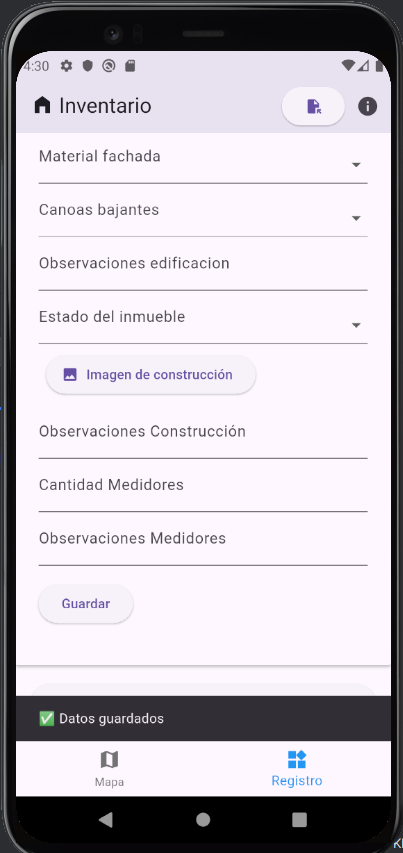
\includegraphics[width=0.3\textwidth]{Graphics/Capitulo 4/Pixel 4 [emulador]/4.4/1.png}
    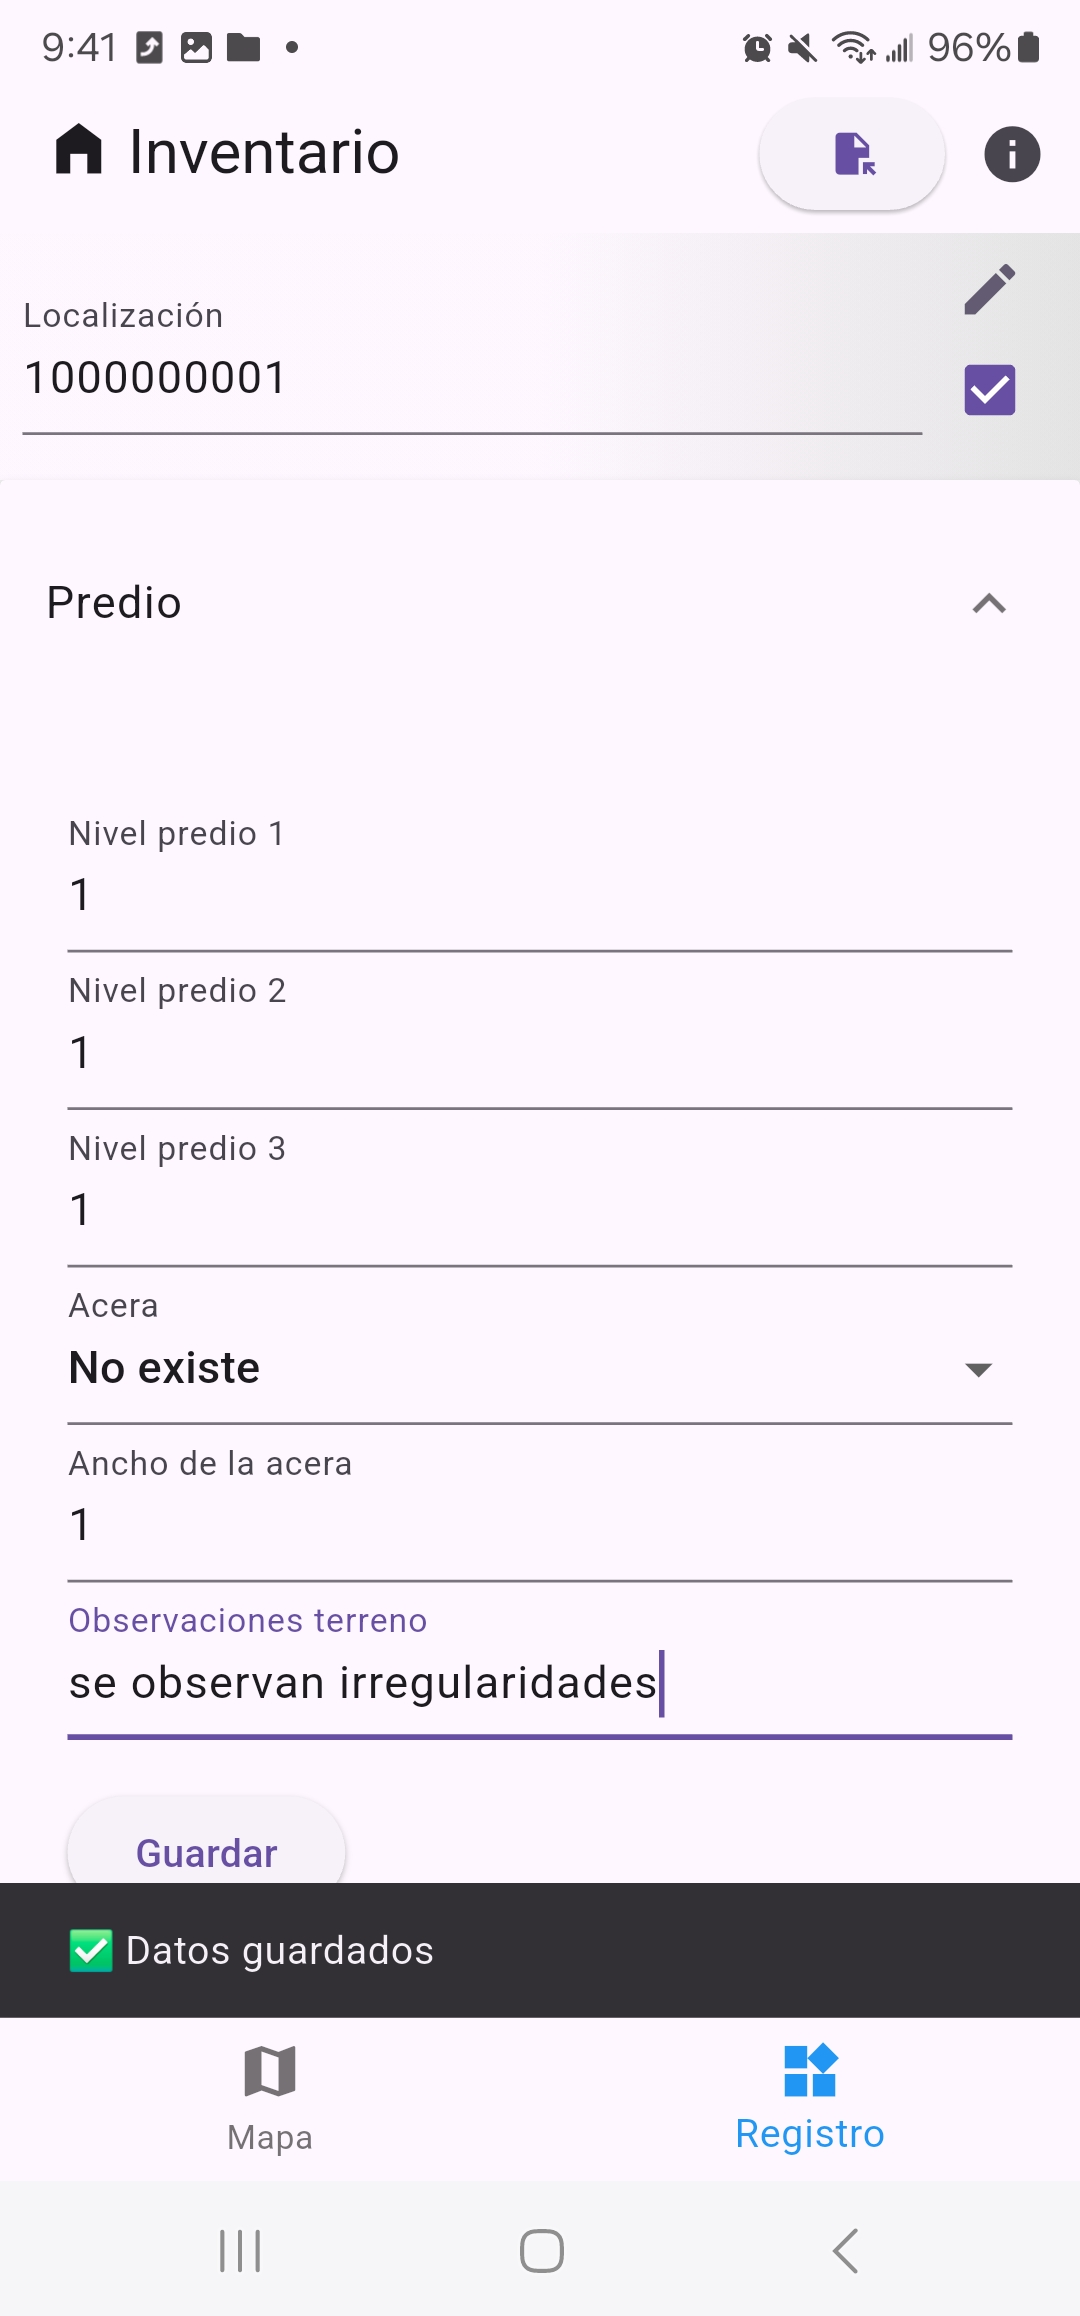
\includegraphics[width=0.3\textwidth]{Graphics/Capitulo 4/Galaxy S23 Ultra Android/4.4/1.jpg}
    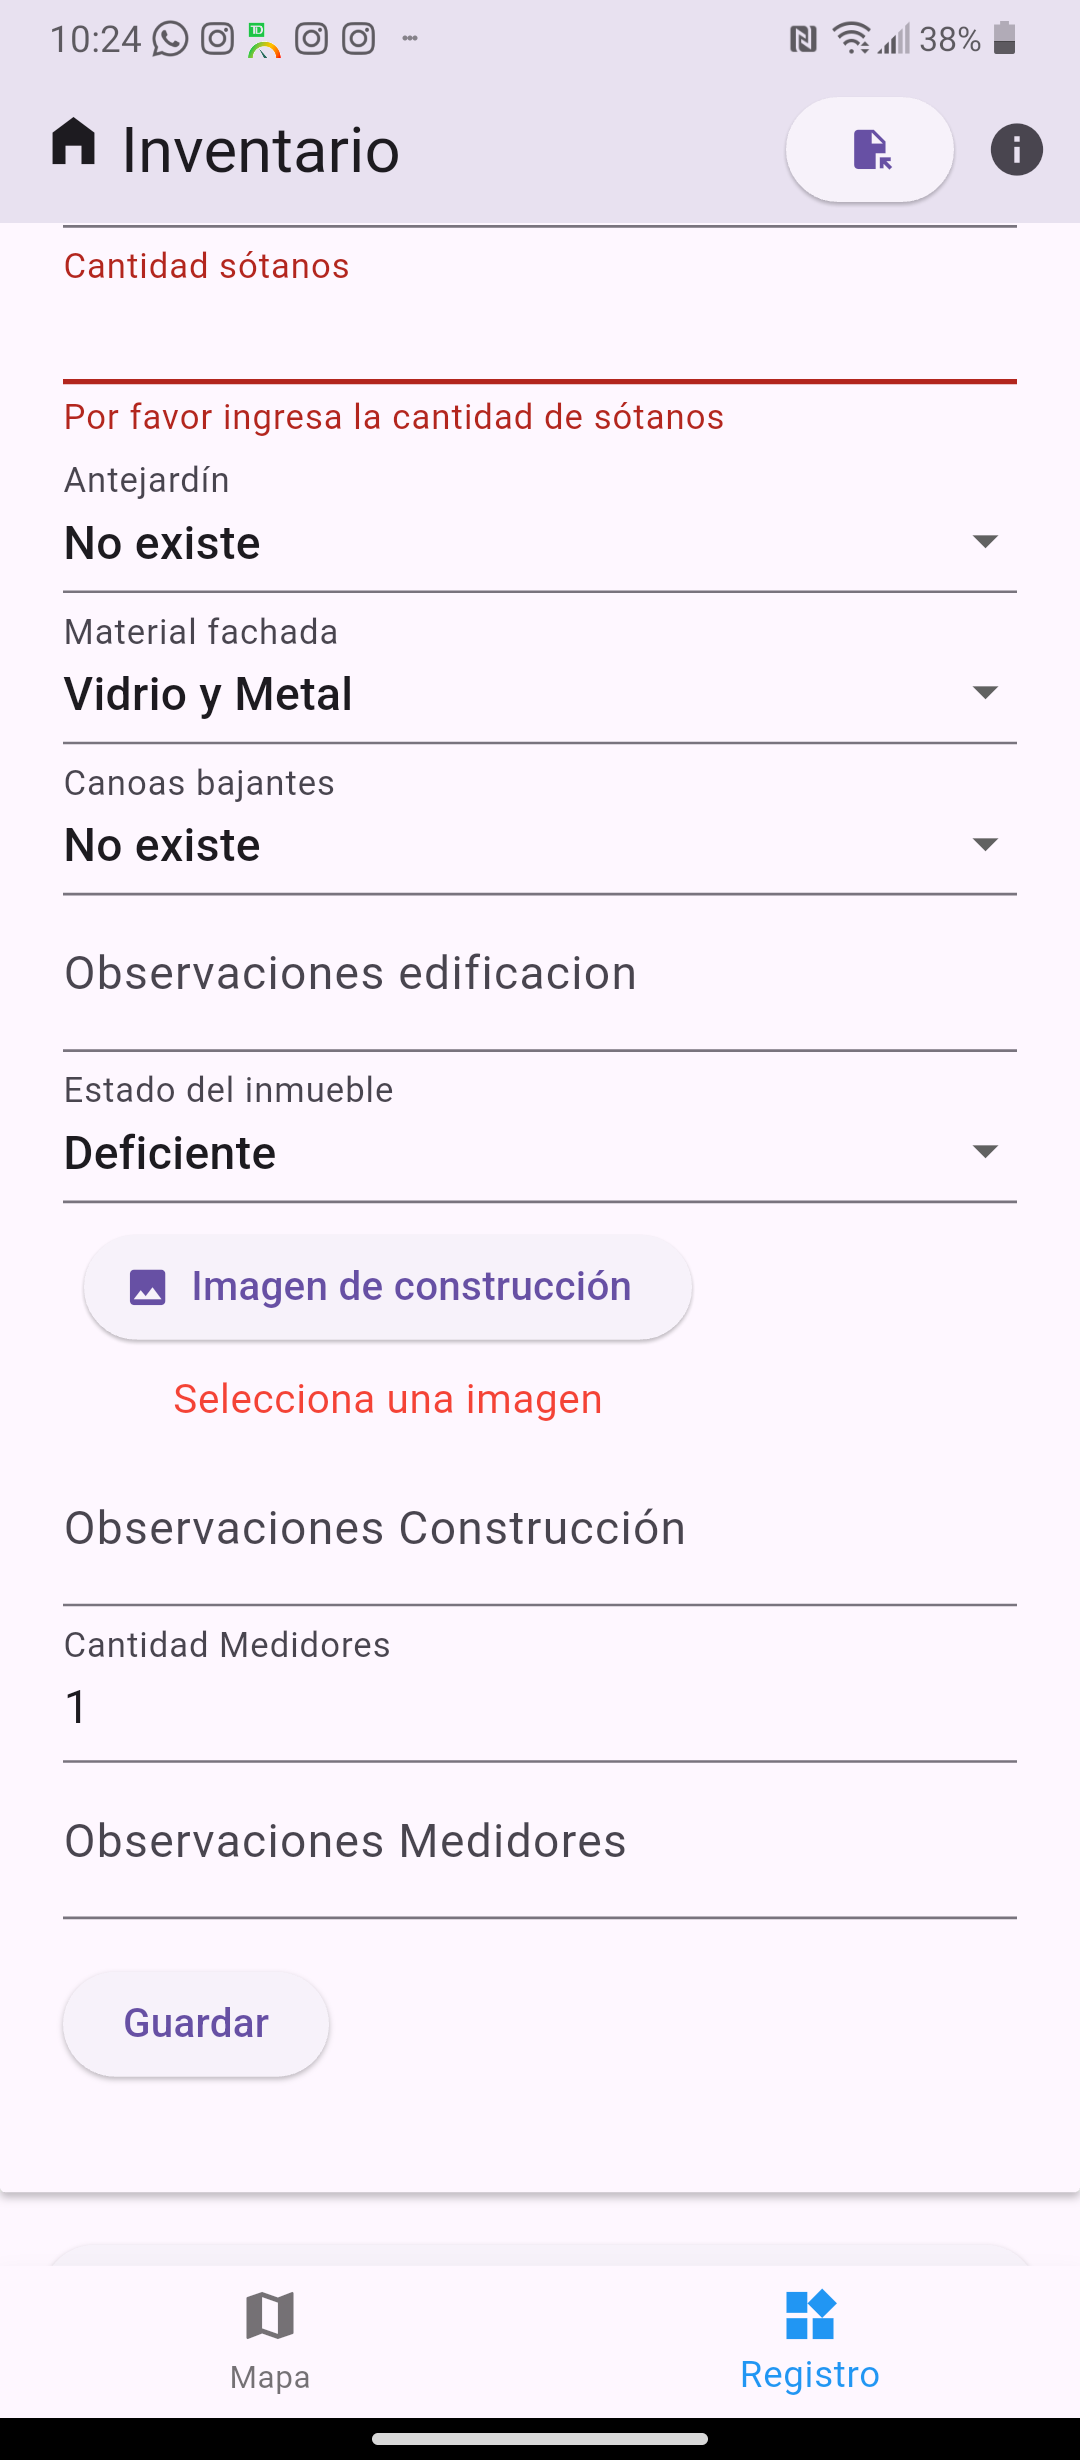
\includegraphics[width=0.3\textwidth]{Graphics/Capitulo 4/LG Android 13/4.4/2.png}
    \caption{Prueba de validación de formularios}
    \label{fig:figura20}
\end{figure}

En esta prueba se pueden ver varios escenarios del proceso de validación de los subformularios. Los campos que se marcaron en rojo no se rellenaron a propósito con el objetivo de mostrar que la
validación funciona. La aplicación sigue teniendo el comportamiento esperado en las tres versiones de Android

\pagebreak
\section{Edición, recuperación y eliminación de Propiedades y Edificios}
\begin{figure}[h]
    % \centering
    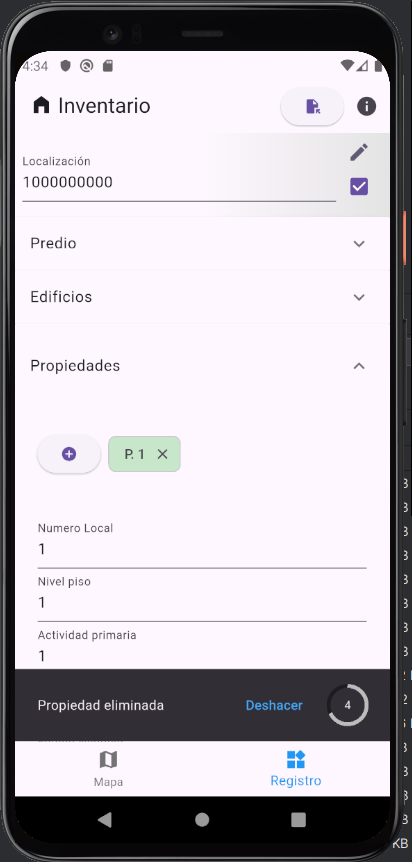
\includegraphics[width=0.3\textwidth]{Graphics/Capitulo 4/Pixel 4 [emulador]/4.5/5.png}
    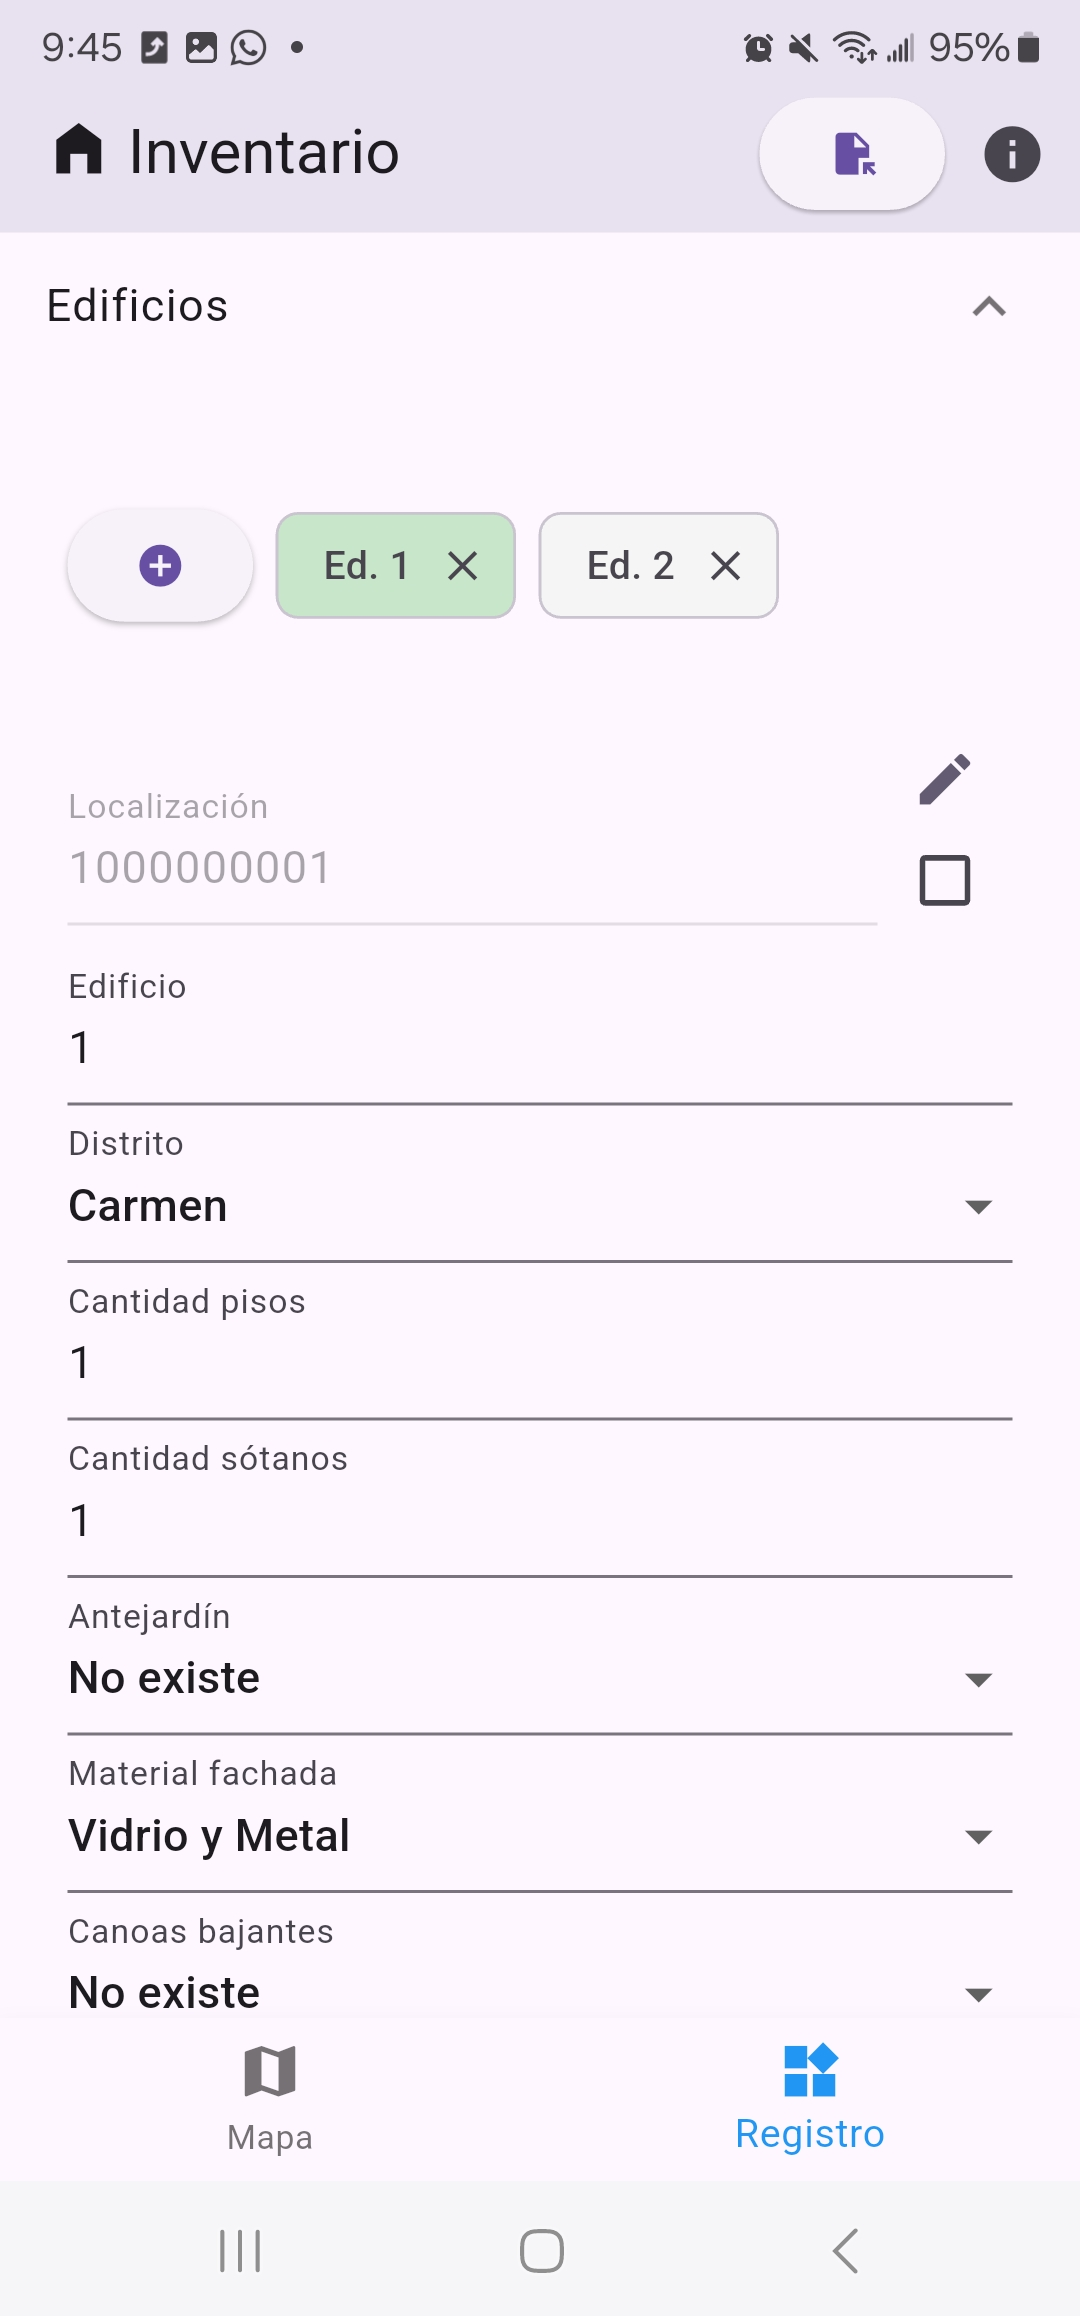
\includegraphics[width=0.3\textwidth]{Graphics/Capitulo 4/Galaxy S23 Ultra Android/4.5/1.jpg}
    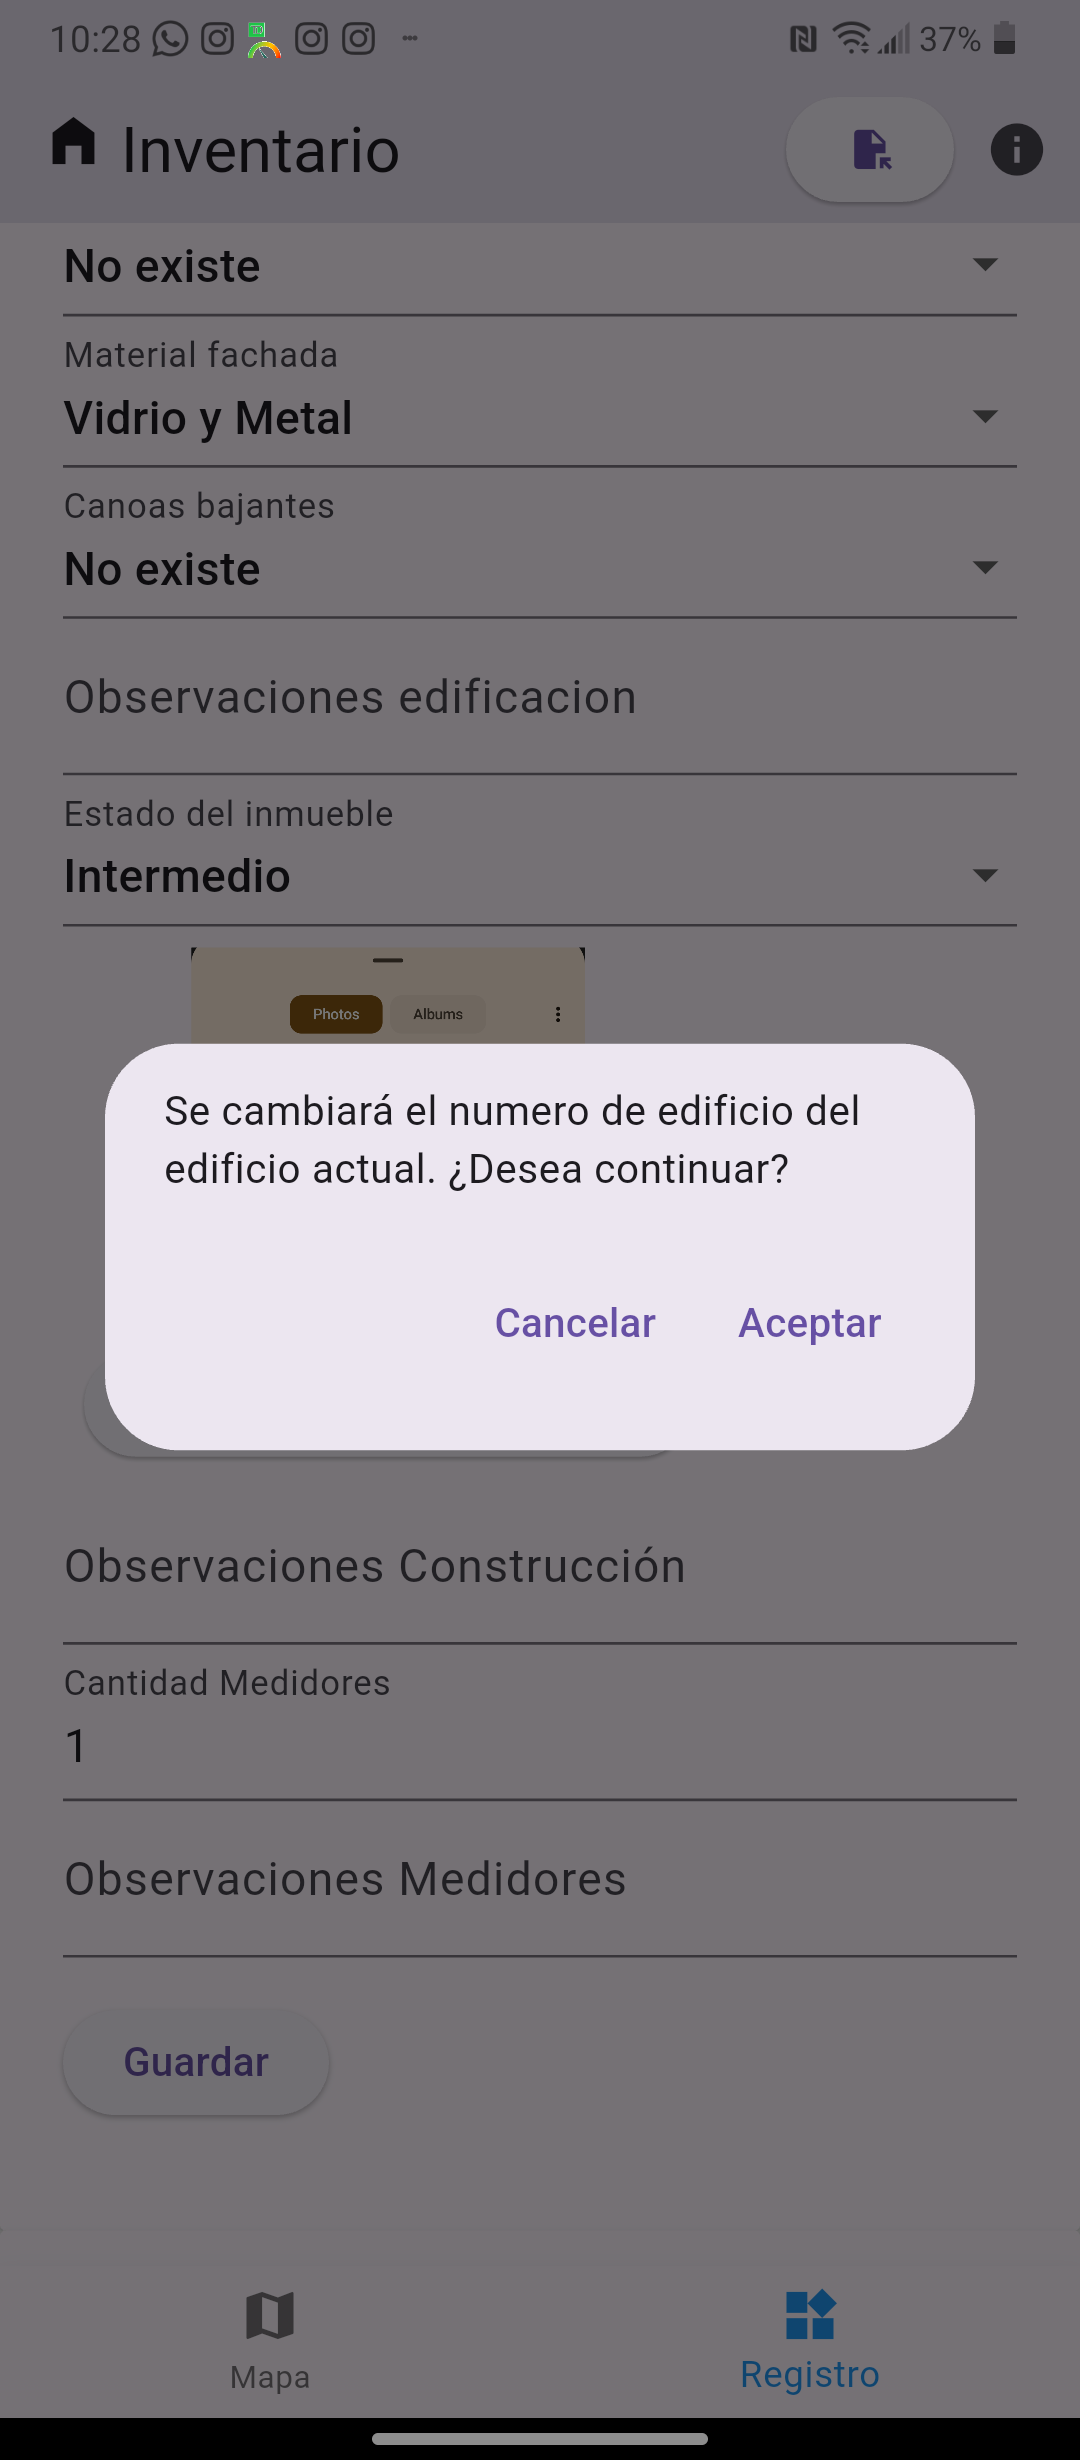
\includegraphics[width=0.3\textwidth]{Graphics/Capitulo 4/LG Android 13/4.4/4.png}
    \caption{Prueba de edición, recuperación y eliminación de Edificios y propiedades}
    \label{fig:figura21}
\end{figure}

En la figura \ref{fig:figura21} se aprecian varios escenarios de edición, eliminación y recuperación de datos de propiedades y edificios. En la imagen de la extrema derecha
se observa un mensaje de confirmación ya que se optó por cambiar el número de edificio de un edificio existente, lo cual es una accion no natural y por ende se agrega un paso de confirmación.
En la imagen de la izquierda, podemos apreciar la eliminación de una entidad. Ya sea Edificio o Propiedad, al eliminar alguna entidad, se eliminará al final de un contador que da la oportunidad
de deshacer la eliminación.

\pagebreak

\section{Marcando varios predios como visitados}
\begin{figure}[h]
    \centering
    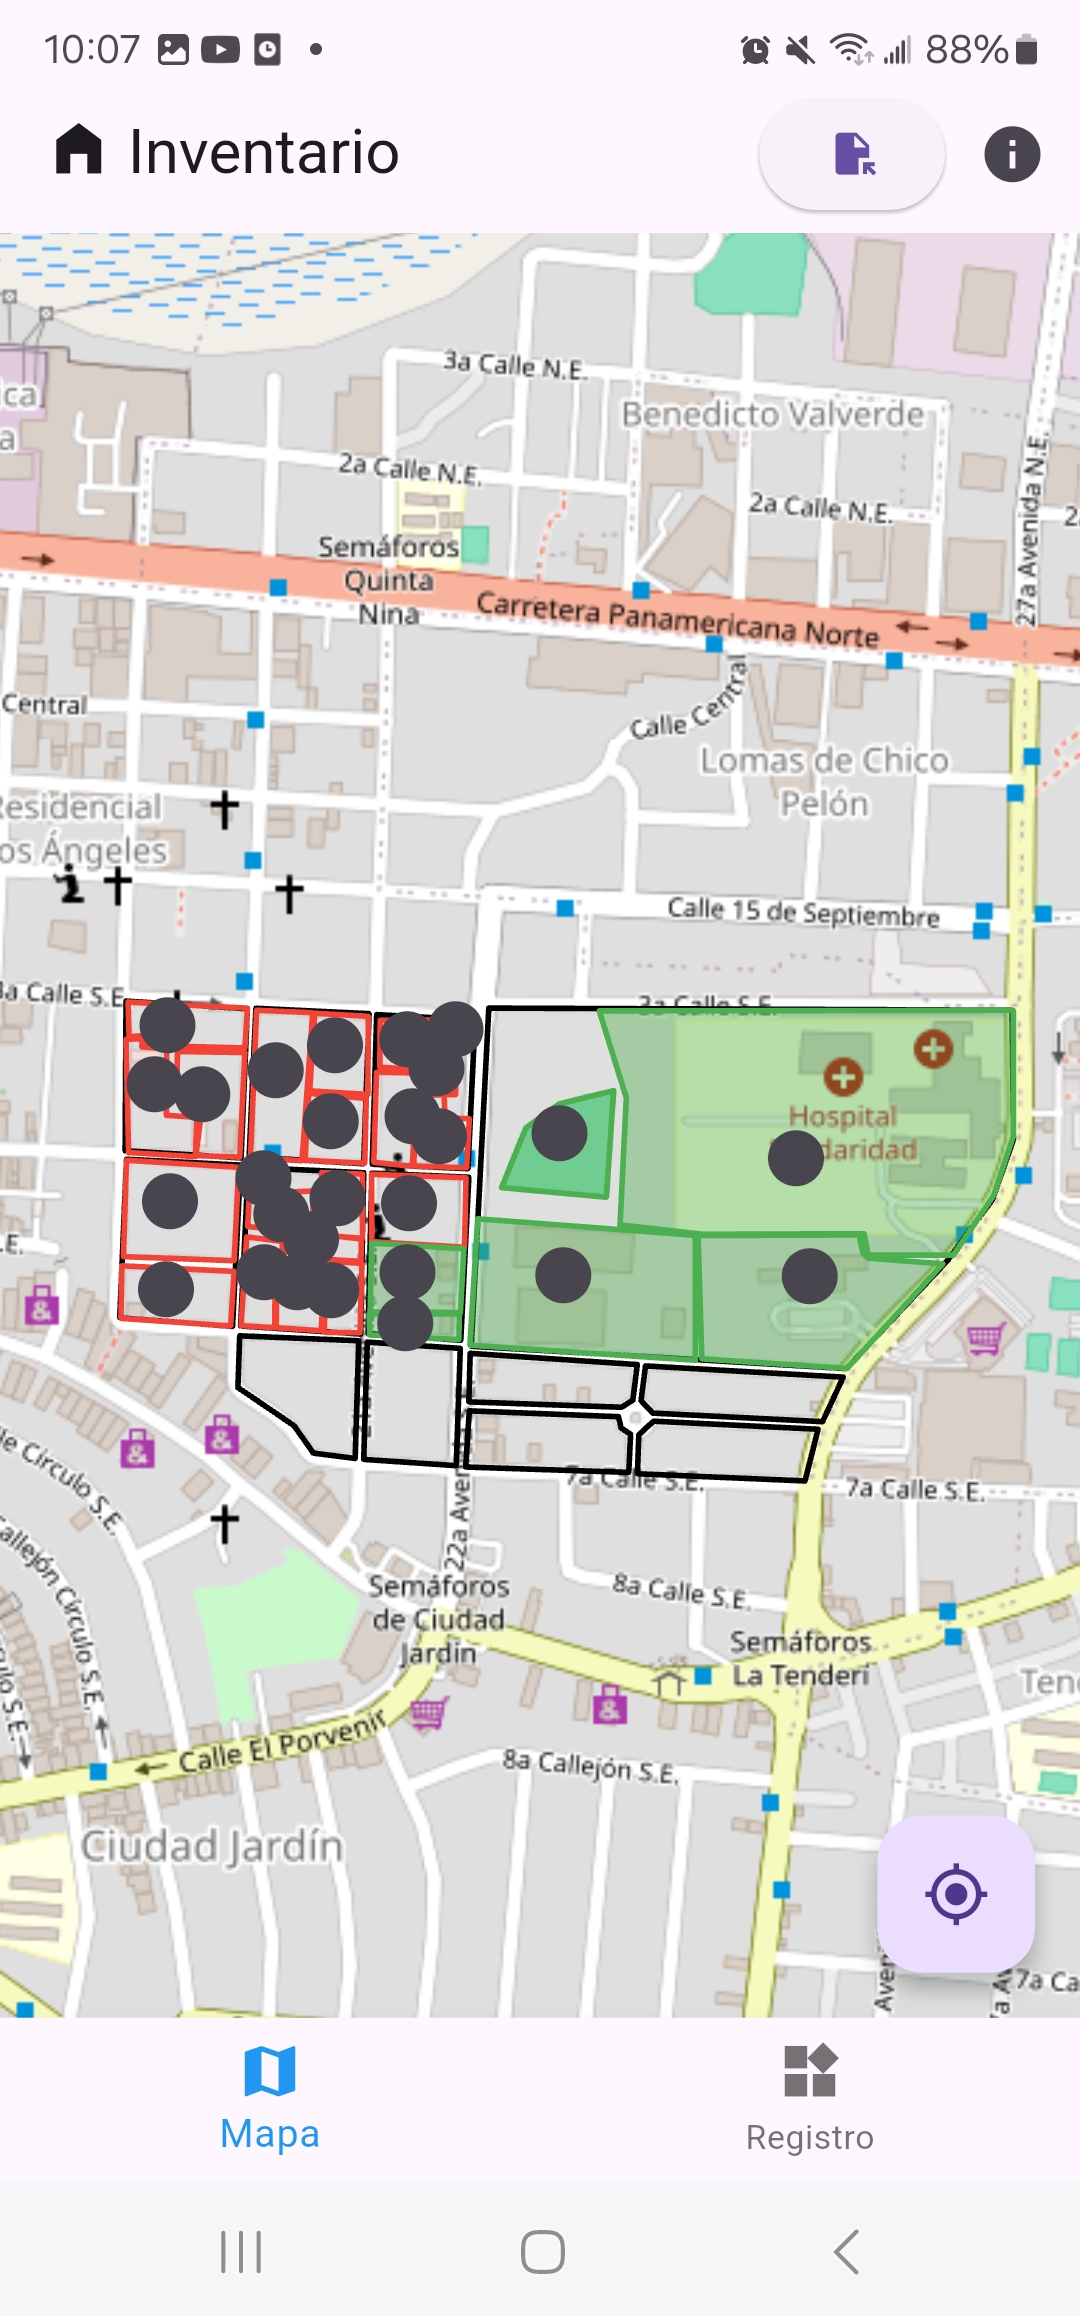
\includegraphics[width=0.3\textwidth]{Graphics/Capitulo 4/Galaxy S23 Ultra Android/4.6/1.jpg}
    \caption{Prueba de la funcionalidad de marcar predios como visitados}
    \label{fig:figura22}
\end{figure}
En la figura \ref{fig:figura22} se pueden observar algunos predios con fondo y bordes verdes, estos fueron marcados como visitados!
\pagebreak
\section{Exportación y Limpieza de la Base de Datos}
\begin{figure}[h]
    \centering
    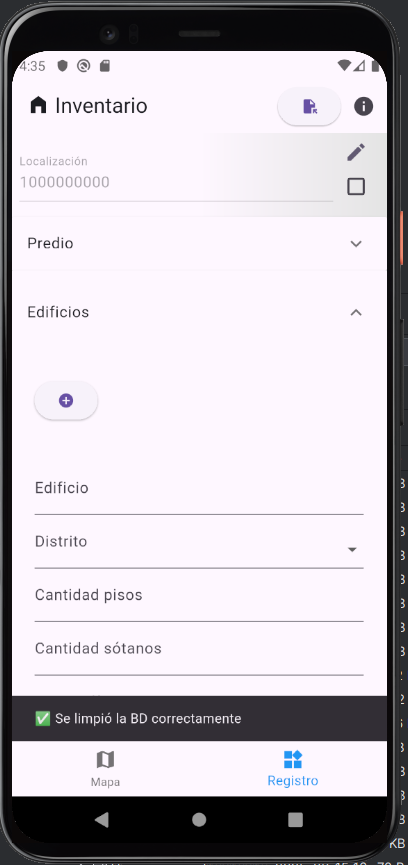
\includegraphics[width=0.3\textwidth]{Graphics/Capitulo 4/Pixel 4 [emulador]/4.7/1.png}
    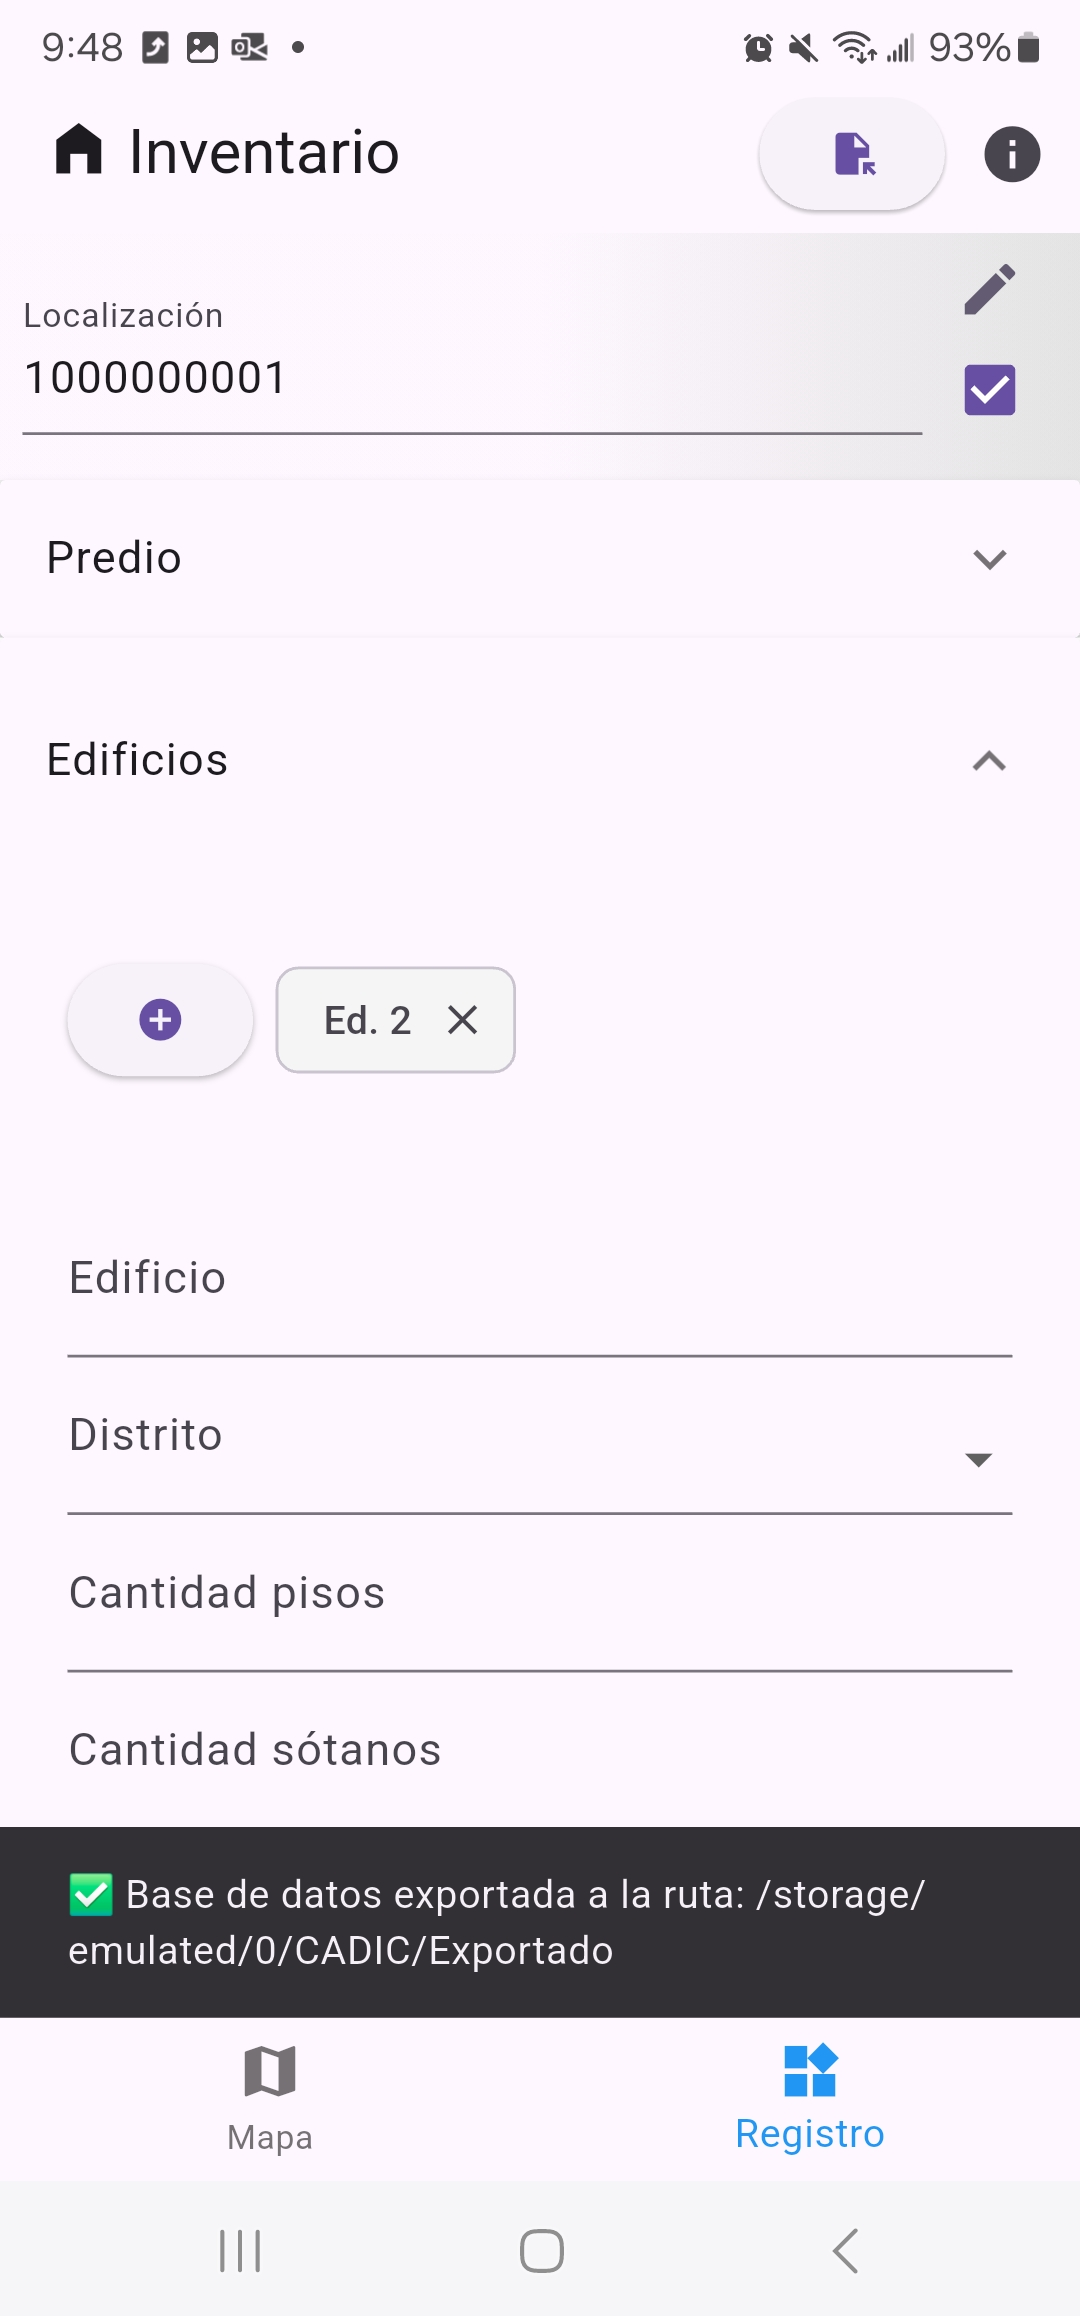
\includegraphics[width=0.3\textwidth]{Graphics/Capitulo 4/Galaxy S23 Ultra Android/4.7/1.jpg}
    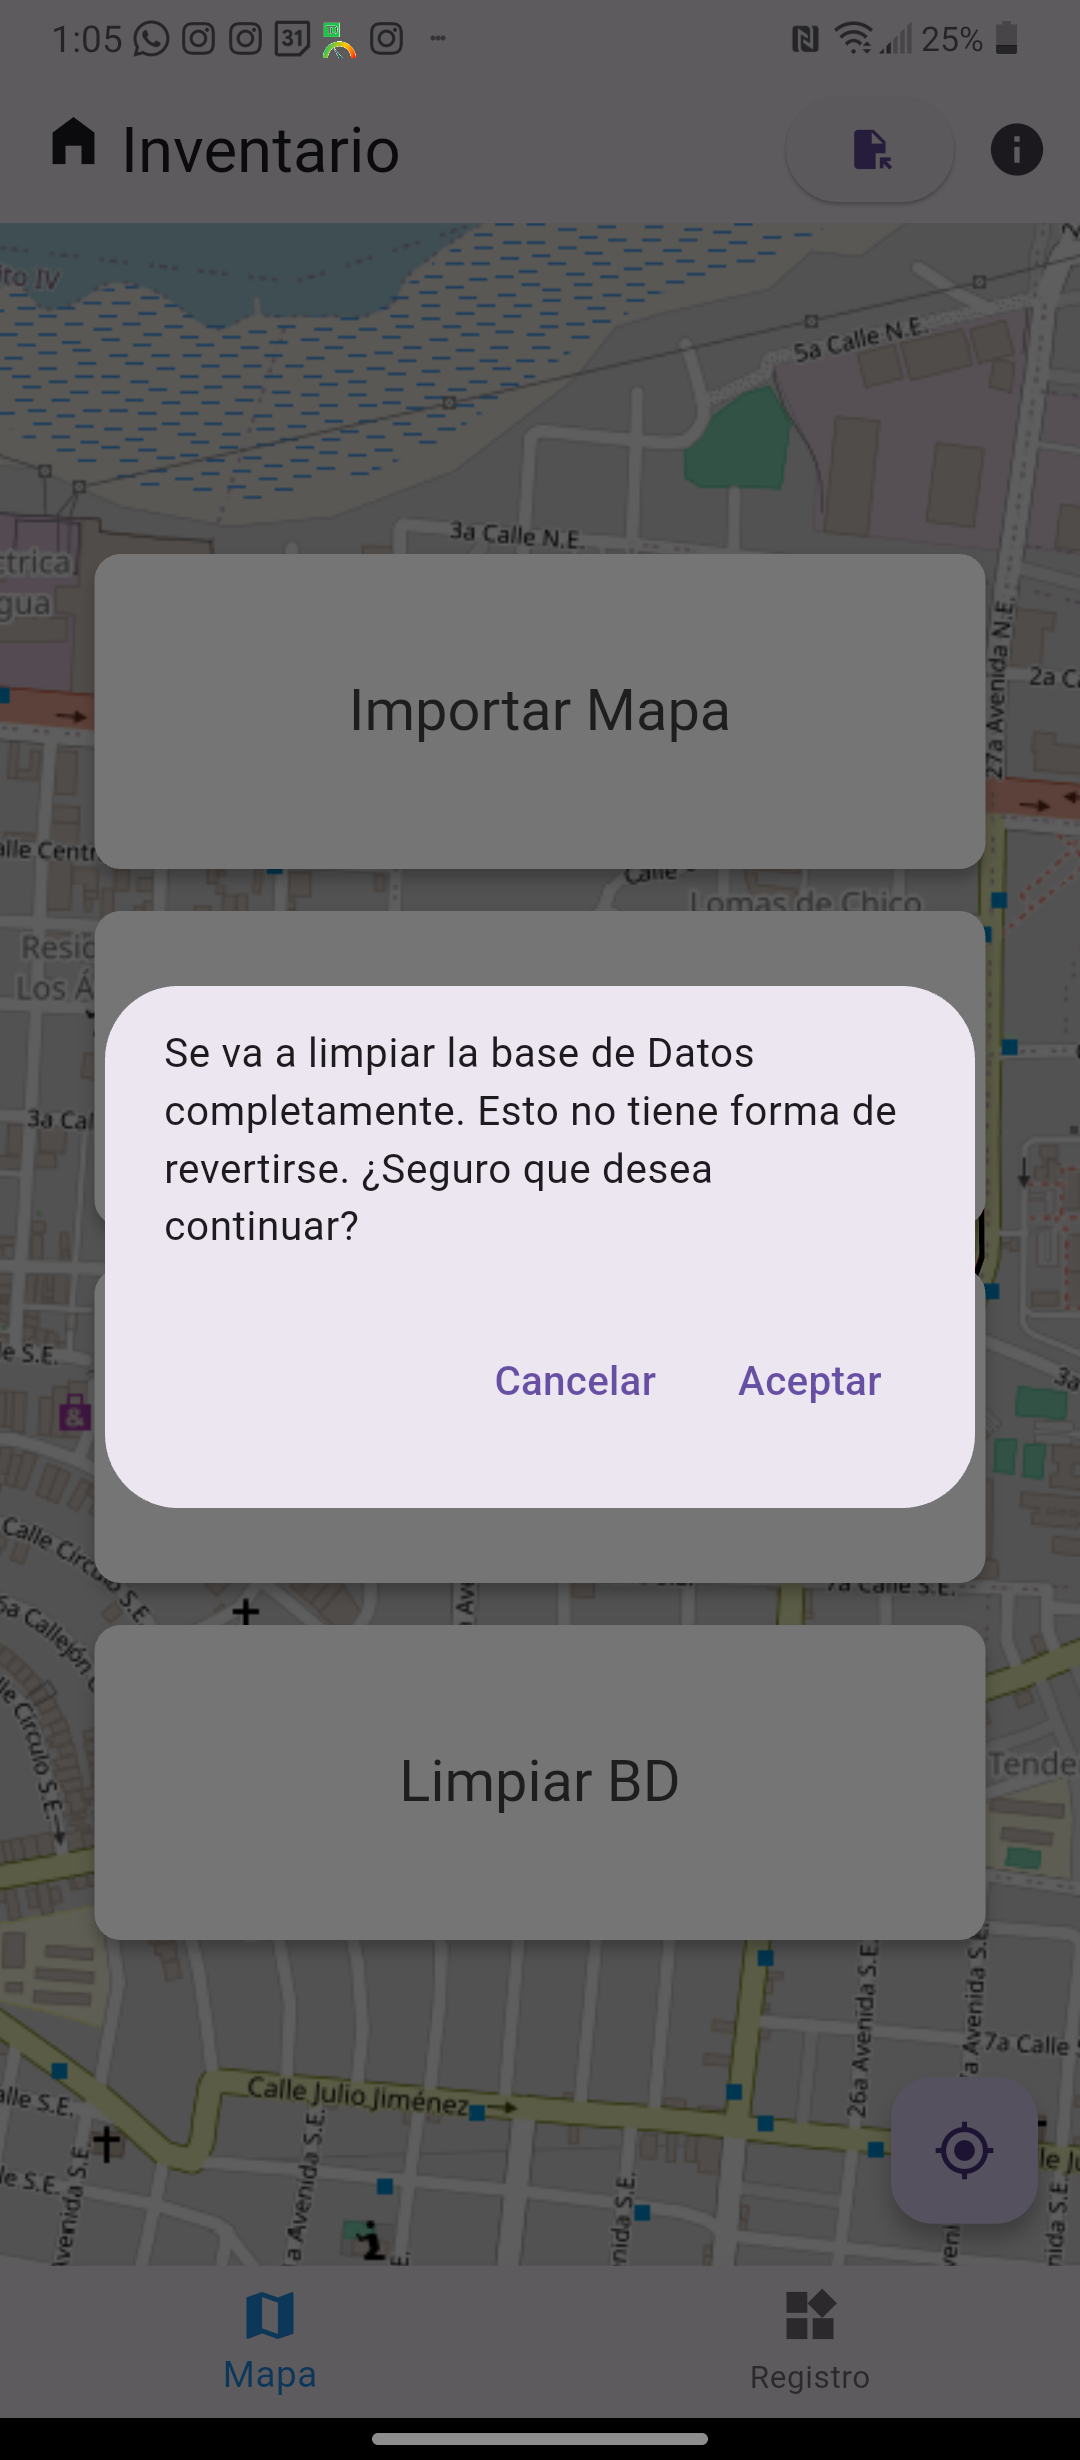
\includegraphics[width=0.3\textwidth]{Graphics/Capitulo 4/LG Android 13/4.7/Screenshot_20250615-130550.png}
    \caption{Prueba de la funcionalidad de marcar predios como visitados}
    \label{fig:figura23}\
    Recalcar que siempre se exporta la base de datos a la misma ruta/directorio: 'CADIC/Exportado' y también importante recalcar que al limpiar la base de datos se eliminan todas las tablas
    excepto la que guarda el nombre del encuestador que está usando la aplicación.
\end{figure}



\backmatter

\begin{conclusions}
    Ya
\end{conclusions}

\begin{recomendations}
    A pesar de haber conseguido nuestro objetivo de manera exitosa, siempre quedan funcionalidades que podrían mejorar y agilizar o hacer más ameno el uso de la aplicación.
    Por ende como recomendaciones podemos incluir:
    \begin{itemize}
        \item Implementar la funcionalidad de la búsqueda del camino más corto para visitar el conjunto de predios asignados a un encuestador.
        \item Implementar la funcionalidad de dejar el mapa estático al cambiar la vista a la pestaña Registro.
    \end{itemize}
\end{recomendations}

\printbibliography[heading=bibintoc]

\end{document}